\documentclass[a4paper]{article}
\usepackage[T1]{fontenc}			% \chapter package
\usepackage[english]{babel}
\usepackage[english]{isodate}  		% date format
\usepackage{graphicx}				% manage images
\usepackage{amsfonts}
\usepackage{booktabs}				% high quality tables
\usepackage{amsmath}				% math package
\usepackage{amssymb}				% another math package (e.g. \nexists)
\usepackage{bm}                     % bold math symbols
\usepackage{mathtools}				% emphasize equations
\usepackage{stmaryrd} 				% '\llbracket' and '\rrbracket'
\usepackage{amsthm}					% better theorems
\usepackage{enumitem}				% manage list
\usepackage{pifont}					% nice itemize
\usepackage{cancel}					% cancel math equations
\usepackage{caption}				% custom caption
\usepackage[]{mdframed}				% box text
\usepackage{multirow}				% more lines in a table
\usepackage{textcomp, gensymb}		% degree symbol
\usepackage[x11names]{xcolor}		% RGB color
\usepackage[many]{tcolorbox}		% colorful box
\usepackage{multicol}				% more rows in a table (used for the lists)
\usepackage{listings}
\usepackage{url}
\usepackage{qrcode}
\usepackage{fontawesome5}
\usepackage{ragged2e}
\usepackage{cite}                   % references
\usepackage{imakeidx}               % index
\usepackage{mfirstuc}               % first letter uppercase
\makeindex[program=makeindex, columns=1,
           title=Index, 
           intoc,
           options={-s index-style.ist}]
\usepackage{fancyhdr}


\definecolor{codegreen}{rgb}{0,0.6,0}
\definecolor{codegray}{rgb}{0.5,0.5,0.5}
\definecolor{codepurple}{rgb}{0.58,0,0.82}
\definecolor{backcolour}{rgb}{0.95,0.95,0.92}
\lstdefinelanguage{misc}
{
  % list of keywords
  morekeywords={%
    add,
    addi,
    lw,
    sw,
    beq,
    bne,
    j,
    jr,
    offset,
    sub,
    and,
    or
  },
  sensitive=false, % keywords are not case-sensitive
  morecomment=[l]{\#}, % l is for line comment
  % morecomment=[s]{/*}{*/}, % s is for start and end delimiter
  % morestring=[b]" % defines that strings are enclosed in double quotes
}
\lstdefinestyle{mystyle}{
    backgroundcolor=\color{backcolour},   
    commentstyle=\color{codegreen},
    keywordstyle=\color{magenta},
    numberstyle=\tiny\color{codegray},
    stringstyle=\color{codepurple},
    basicstyle=\ttfamily\footnotesize,
    breakatwhitespace=false,         
    breaklines=true,                 
    captionpos=b,                    
    keepspaces=true,                 
    numbers=left,                    
    numbersep=5pt,                  
    showspaces=false,                
    showstringspaces=false,
    showtabs=false,                  
    tabsize=2
}
\lstset{style=mystyle}



% draw a frame around given text
\newcommand{\framedtext}[1]{%
	\par%
	\noindent\fbox{%
		\parbox{\dimexpr\linewidth-2\fboxsep-2\fboxrule}{#1}%
	}%
}


% table of content links
\usepackage{xcolor}
\usepackage[linkcolor=black, citecolor=blue, urlcolor=cyan]{hyperref} % hypertexnames=false
\hypersetup{
	colorlinks=true
}


\newtheorem{theorem}{\textcolor{Red3}{\underline{Theorem}}}
\renewcommand{\qedsymbol}{QED}
\newcommand{\dquotes}[1]{``#1''}
\newcommand{\longline}{\noindent\rule{\textwidth}{0.4pt}}
\newcommand{\circledtext}[1]{\raisebox{.5pt}{\textcircled{\raisebox{-.9pt}{#1}}}}
\newcommand{\definition}[1]{\textcolor{Red3}{\textbf{#1}}}
\newcommand{\example}[1]{\textcolor{Green4}{\textbf{#1}}}
\newcommand{\highspace}{\vspace{1.2em}\noindent}
\ExplSyntaxOn
\NewDocumentCommand{\indexdefinition}{m}{%
  \textcolor{Red3}{\textbf{#1}}%
  \index{\char_titlecase:N #1} % add the index entry
}
\ExplSyntaxOff


\begin{document}
    \newcounter{definition}[section]
    \newcounter{example}[section]
    
    \newtcolorbox[use counter = definition]{definitionbox}[1][]{%
        breakable,
        enhanced,    
        colback=red!5!white,
        colframe=red!75!black,
        fonttitle=\bfseries,
        title={Definition \thetcbcounter #1} %
    }
    
    \newtcolorbox[use counter = example]{examplebox}[1][]{%
        breakable,
        enhanced,
        colback=Green4!5!white,
        colframe=Green4!75!black,
        fonttitle=\bfseries,
        title={Example \thetcbcounter #1} %
    }
	
    %%%%%%%%%%%%%%%
    % Notes cover %
    %%%%%%%%%%%%%%%
    \author{260236}
\title{Software Engineering for HPC - Notes}
\date{\printdayoff\today}
\maketitle

    %%%%%%%%%%%
    % Preface %
    %%%%%%%%%%%
    \section*{Preface}

Every theory section in these notes has been taken from two sources:
\begin{itemize}
    \item None
\end{itemize}
About:
\begin{itemize}
    \item[\faIcon{github}] \href{https://github.com/PoliMI-HPC-E-notes-projects-AndreVale69/HPC-E-PoliMI-university-notes}{GitHub repository}
\end{itemize}

    %%%%%%%%%%%%%%%%%%%%%
    % Table of contents %
    %%%%%%%%%%%%%%%%%%%%%
	\tableofcontents
    \newpage

    %%%%%%%%%%%%%%%%%%%
    % Fancy pagestyle %
    %%%%%%%%%%%%%%%%%%%
    \pagestyle{fancy}
    \fancyhead{} % clear all header fields
    \fancyhead[R]{\nouppercase{\leftmark\hfill\rightmark}}

    %%%%%%%%%%%%%%%%%%
    % Basic concepts %
    %%%%%%%%%%%%%%%%%%
    \section{Basic Concepts}

This section is designed to review old concepts that are fundamental to this course.

\subsection{Pipelining}

\subsubsection{MIPS  Architecture}

\definition{MIPS} (\textbf{Microprocessor without Interlocked Pipelined Stages}) is a family of Reduced Instruction Set Computer (RISC). It is based on the concept of \textbf{executing only simple instruction in a reduced basic cycle to optimize the performance of CISC}\footnote{CISC processors use simple and complex instructions to complete any given task. Instead, the RISC processor uses the approach of increasing internal parallelism by executing a simple set of instructions in a single clock cycle (see more \href{https://electronicsdesk.com/cisc-processor.html}{here}).} CPUs.

\highspace
MIPS is a \textbf{load-store architecture} (or a register–register architecture), which means it is an Instruction Set Architecture (ISA\footnote{Instruction Set Architecture (ISA) is a part of the abstract model of a computer, which generally defines how software controls the CPU.}) that divides \textbf{instructions into two categories}: 
\begin{itemize}
    \item \textbf{Memory access} (load and store between memory and registers; load data from memory to registers; store data from registers to memory):
    \begin{equation*}
        \begin{array}{rcl}
            \text{Memory } &\xlongrightarrow{\mathbf{load}}& \text{ Registers} \\ [.5em]
            \text{Memory } &\xlongleftarrow{\mathbf{store}}& \text{ Registers}
        \end{array}
    \end{equation*}
    \item ALU operations (which only occur between registers).
\end{itemize}

\highspace
Finally, \textbf{MIPS} is also a \textbf{Pipeline Architecture}. It means that \textbf{it can execute a performance optimization technique based on overlapping the execution of multiple instructions derived from a sequential execution flow}.

\newpage

\begin{center}
    \large
    \textcolor{Red3}{\textbf{Reduced Instruction Set of MIPS Processor}}
\end{center}
The instruction set of the MIPS processor is the following:
\begin{itemize}
    \item \underline{ALU instructions}:
    \begin{itemize}
        \item \textbf{Sum} between \textbf{two registers}:
        \lstinputlisting[language=misc]{code/mips-architecture/add.s}
        Take the values from \texttt{s2} and \texttt{s3}, make the sum and save the result on \texttt{s1}.

        \item \textbf{Sum} between \textbf{register and constant}:
        \lstinputlisting[language=misc]{code/mips-architecture/addi.s}
        Take the value from \texttt{s1}, make the sum between \texttt{s1} and \texttt{4}, and save the result on \texttt{s1}.
    \end{itemize}

    \item \underline{Load/Store instructions}:
    \begin{itemize}
        \item \textbf{Load}
        \lstinputlisting[language=misc]{code/mips-architecture/load.s}
        From the \texttt{s2} register, calculate the index on the memory with the \texttt{offset}, take the value and store it in the \texttt{s1} register.

        \item \textbf{Store}
        \lstinputlisting[language=misc]{code/mips-architecture/store.s}
        Take the value from the \texttt{s1} register, take the value from the \texttt{s2} register, calculate the index on the memory with the \texttt{offset}, and store the value taken from s1 in the memory.
    \end{itemize}

    \item \underline{Branch instructions to control the instruction flow}:
    \begin{itemize}
        \item \textbf{Conditional branches}
        
        Only if the condition is true (branch on equal):
        \lstinputlisting[language=misc]{code/mips-architecture/beq.s}
        
        Only if the condition is false (branch on not equal):
        \lstinputlisting[language=misc]{code/mips-architecture/bne.s}


        \item \textbf{Unconditional jumps}. The branch is always taken.

        Jump:
        \lstinputlisting[language=misc]{code/mips-architecture/j.s}

        Jump register:
        \lstinputlisting[language=misc]{code/mips-architecture/jr.s}
    \end{itemize}
\end{itemize}

\newpage

\begin{center}
    \large
    \textcolor{Red3}{\textbf{Formats of MIPS 32-bit Instructions}}
\end{center}
The previous instructions are divided into \textbf{three types}: 
\begin{itemize}
    \item Type \textbf{R (Register)}: ALU instructions.

    \item Type \textbf{I (Immediate)}: Load/Store instructions and Conditional branches.
    
    \item Type \textbf{J (Jump)}: Unconditional jumps instructions.
\end{itemize}
Every instruction \textbf{starts with a 6-bit opcode}. In addition to the opcode:
\begin{itemize}
    \item \underline{R-type} instructions specify:
    \begin{itemize}
        \item \textbf{Three registers}: \texttt{rs}, \texttt{rt}, \texttt{rd}
        \item A \textbf{shift amount field}: \texttt{shamt}
        \item A \textbf{function field}: \texttt{funct}
    \end{itemize}

    \item \underline{I-type} instructions specify:
    \begin{itemize}
        \item \textbf{Two registers}: \texttt{rs}, \texttt{rt}
        \item \textbf{16-bit immediate value}: \texttt{offset/immediate}
    \end{itemize}

    \item \underline{J-type} instructions specify: 
    \begin{itemize}
        \item \textbf{26-bit jump target}: \texttt{address}
    \end{itemize}
\end{itemize}

\begin{figure}[!htp]
    \centering
    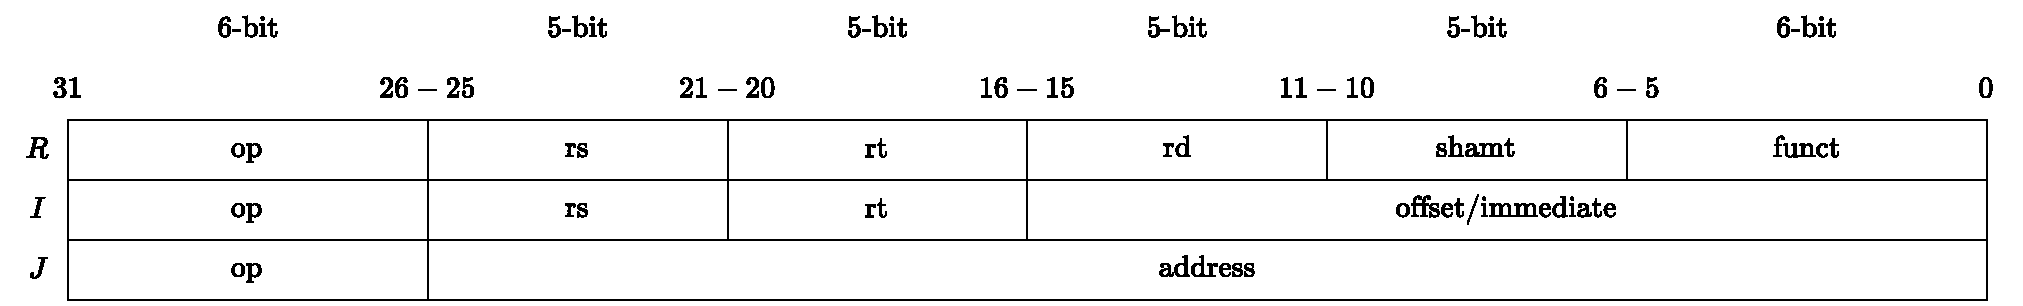
\includegraphics[width=\textwidth]{img/mips-arch.pdf}
    \caption{MIPS 32-bit architecture.}
\end{figure}

\noindent
Scan (or click) the QR code below to view the table in high quality:
\begin{center}
    \qrcode{https://github.com/AndreVale69/HPC-E-PoliMI-university-notes/tree/main/advanced-computer-architectures/notes/img/mips-arch.pdf}
\end{center}

\newpage

\begin{center}
    \large
    \textcolor{Red3}{\textbf{Phases of execution of MIPS Instructions}}
    \index{Program Counter (PC)}
    \index{Instruction Memory (IM)}
    \index{Register File (RF)}
    \index{Data Memory (DM)}
    \label{Phases of execution of MIPS Instructions}
\end{center}
Every instruction in the MIPS subset can be implemented in \textbf{\underline{at most} 5 clock cycles (phases)} as follows:
\begin{enumerate}
    \item \definition{Instruction Fetch (IF)}
    \begin{enumerate}
        \item \textbf{Send} the \textbf{content} of Program Counter (PC) register to the Instruction Memory (IM);

        \item \textbf{Fetch} the current \textbf{instruction} from Instruction Memory;
        
        \item \textbf{Update} the Program Counter to the \textbf{next sequential address} by adding the value 4 to the Program Counter (4 because each instruction is 4 bytes!).
    \end{enumerate}
    
    \item \definition{Instruction Decode and Register Read (ID)}
    \begin{enumerate}
        \item Make the \textbf{fixed-filed recording} (\textbf{decode the current instruction});
        
        \item \textbf{Read} from the Register File (RF) of one or two registers corresponding to the registers specified in the instruction fields;
        
        \item Sign-extension of the offset field of the instruction in case it is needed.
    \end{enumerate}

    \item \definition{Execution (EX)}. The ALU operates on the operands prepared in the previous cycle depending on the instruction type (see more details after this list):
    \begin{itemize}
        \item \textbf{Register-Register} ALU instructions: ALU \textbf{executes the specified operation} on the operands read from the Register File.

        \item \textbf{Register-Immediate} (Register-Constant) ALU instructions: ALU executes the specified operation on the first operand read from Register File and the sign-extended immediate operand.

        \item \textbf{Memory Reference}: ALU adds the base register and the offset to calculate the \textbf{effective address}.

        \item \textbf{Conditional Branches}: ALU compares the two registers read from Register File and computes the possible \textbf{branch target address} by adding the sign-extended offset to the incremented Program Counter.
    \end{itemize}

    \item \definition{Memory Access (ME)}. It depends on the operation performed:
    \begin{itemize}
        \item \underline{\textbf{Load}}. Instructions require a \textbf{read access to the Data Memory using the effective address}.

        \item \underline{\textbf{Store}}. Instruction require a \textbf{write access to the Data Memory using the effective address} to write the data \textbf{from the source register read from the Register File}.

        \item \underline{\textbf{Conditional branches}} can \textbf{update the content of the Program Counter} with the branch target address, if the conditional test yielded true.
    \end{itemize}

    \newpage

    \item \definition{Write-Back (WB)}. It depends on the operation performed:
    \begin{enumerate}
        \item \underline{\textbf{Load}} instructions \textbf{write the data read from memory in the destination register of the Register File}.

        \item \underline{\textbf{ALU}} instructions \textbf{write the ALU results into the destination register of the Register File}.
    \end{enumerate}
\end{enumerate}

\begin{flushleft}
    \textcolor{Red3}{\textbf{Execution (EX) details}}\label{Execution (EX) details}
\end{flushleft}
\begin{itemize}
    \item \textbf{Register-Register ALU instructions}. Given the following pattern (where \texttt{op} can be the operators \texttt{add/addi} (+) or \texttt{sub/subi} (-), but not \texttt{mult} ($\times$) or \texttt{div} ($\div$) because they required some special registers and therefore more phases):
    \lstinputlisting[language=misc]{code/mips-architecture/alu-instructions-1.s}
    \textbf{Cost: 4 clock cycles}
    \begin{enumerate}
        \item Instruction Fetch (IF) and update the Program Counter (next sequential address);

        \item Fixed-Field Decoding and read from Register File the registers: \texttt{y} and \texttt{z};
        
        \item Execution (EX), ALU performs the operation \texttt{op} (\texttt{\$ y op \$ z});

        \item Write-Back (WB), ALU writes the result into the destination register \texttt{x}.
    \end{enumerate}

    \item \textbf{Memory Reference}
    \begin{itemize}
        \item \underline{Load}. Given the following pattern:
        \lstinputlisting[language=misc]{code/mips-architecture/alu-instructions-2.s}
        \textbf{Cost: 5 clock cycles}
        \begin{enumerate}
            \item Instruction Fetch (IF) and update the Program Counter (next sequential address);

            \item Fixed-Field Decoding and read of Base and register \texttt{y} from Register File (RF);

            \item Execution (EX), ALU adds the base register and the offset to calculate the effective address: \texttt{y + offset};

            \item Memory Access (ME), read access to the Data Memory (DM) using the effective (\texttt{y + offset}) address;

            \item Write-Back (WB), write the data read from memory in the destination register of the Register File (RF) \texttt{x}.
        \end{enumerate}

        \newpage

        \item \underline{Store}. Given the following pattern:
        \lstinputlisting[language=misc]{code/mips-architecture/alu-instructions-3.s}
        \textbf{Cost: 4 clock cycles}
        \begin{enumerate}
            \item Instruction Fetch (IF) and update the Program Counter (next sequential address);

            \item Fixed-Field Decoding and read of Base register \texttt{y} and source register \texttt{x} from Register File (RF);

            \item Execution (EX), ALU adds the base register and the offset to calculate the effective address: \texttt{y + offset};

            \item Memory Access (WB), write the data read from memory in the destination register of the Register File (RF) \texttt{M(y + offset)}.
        \end{enumerate}
    \end{itemize}

    \item \textbf{Conditional Branch}. Given the following pattern:
    \lstinputlisting[language=misc]{code/mips-architecture/alu-instructions-4.s}
        \textbf{Cost: 4 clock cycles}
        \begin{enumerate}
            \item Instruction Fetch (IF) and update the Program Counter (next sequential address);

            \item Fixed-Field Decoding and read of source registers \texttt{x} and \texttt{y} from Register File (RF);

            \item Execution (EX), ALU compares two registers \texttt{x} and \texttt{y} and compute the possible branch target address by adding the sign-extended offset to the incremented Program Counter: \texttt{PC + 4 + offset};

            \item Memory Access (ME), update the content of the Program Counter with the branch target address (we assume that the conditional test is true).
        \end{enumerate}
\end{itemize}
    \subsubsection{Implementation of MIPS processor - Data Path}

Implementing a MIPS processor isn't difficult. On the following page we show three different diagrams: the first is a very high level data path to allow the reader to understand how it works; the second is more detailed, but without the CU (Control Unit); the third is the complete data path and it also includes the CU (in red).

\begin{figure}[!htp]
    \centering
    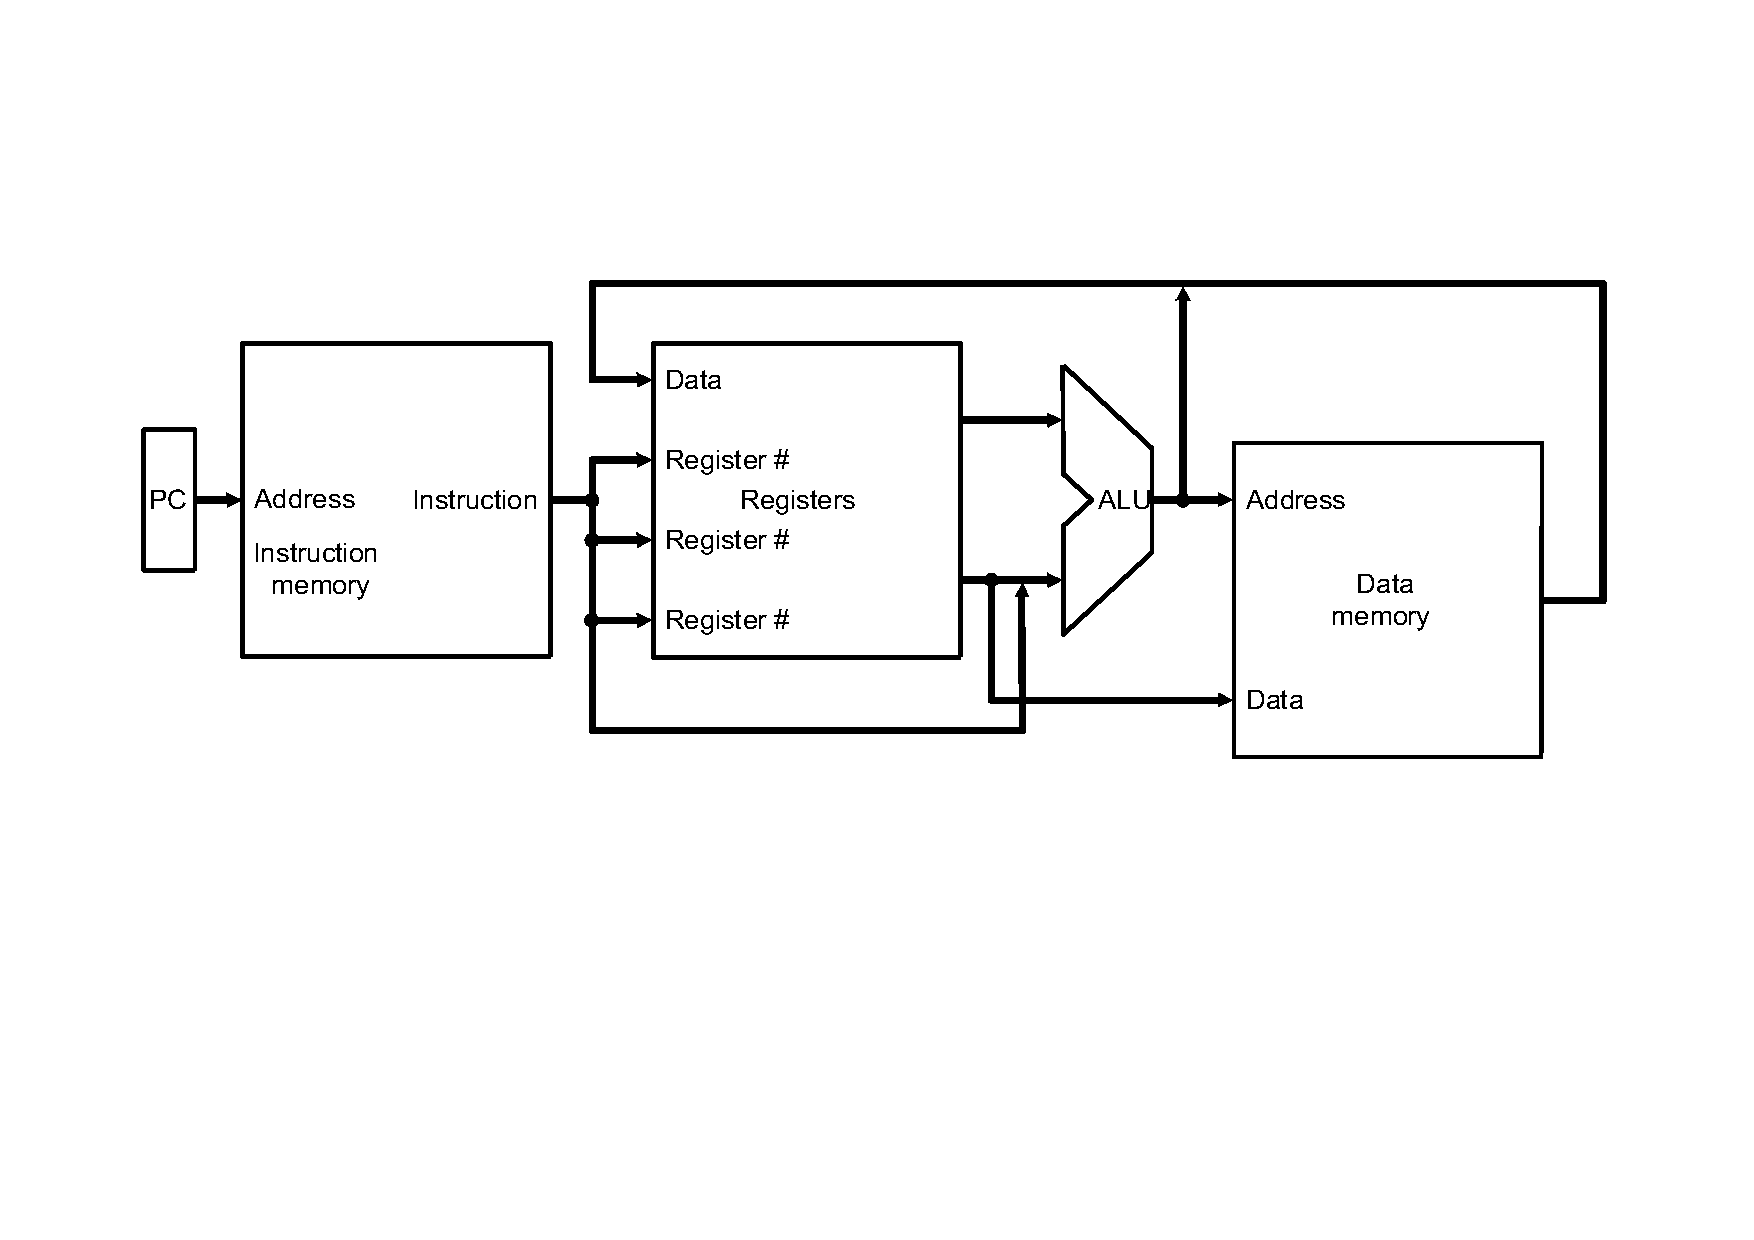
\includegraphics[width=\textwidth]{img/basic-implementation-mips-datapath.pdf}
    \caption{A basic implementation of MIPS data path.\cite{pipelining-slides}}
    \label{fig: basic implementation of MIPS data path}
\end{figure}

\noindent
Scan (or click) the QR code below to view the figure~\ref{fig: basic implementation of MIPS data path} in high quality:
\begin{center}
    \qrcode{https://github.com/PoliMI-HPC-E-notes-projects-AndreVale69/HPC-E-PoliMI-university-notes/tree/main/advanced-computer-architectures/notes/img/basic-implementation-mips-datapath.pdf}
\end{center}
Two notes:
\begin{itemize}
    \item The \textbf{Instruction Memory} (read-only memory) is separated from \textbf{Data Memory}.
    
    \item The 32 general-purpose register are organized in a \textbf{Register File} (RF) with 2 read ports and 1 write port.
\end{itemize}

\begin{figure}[!htp]
    \centering
    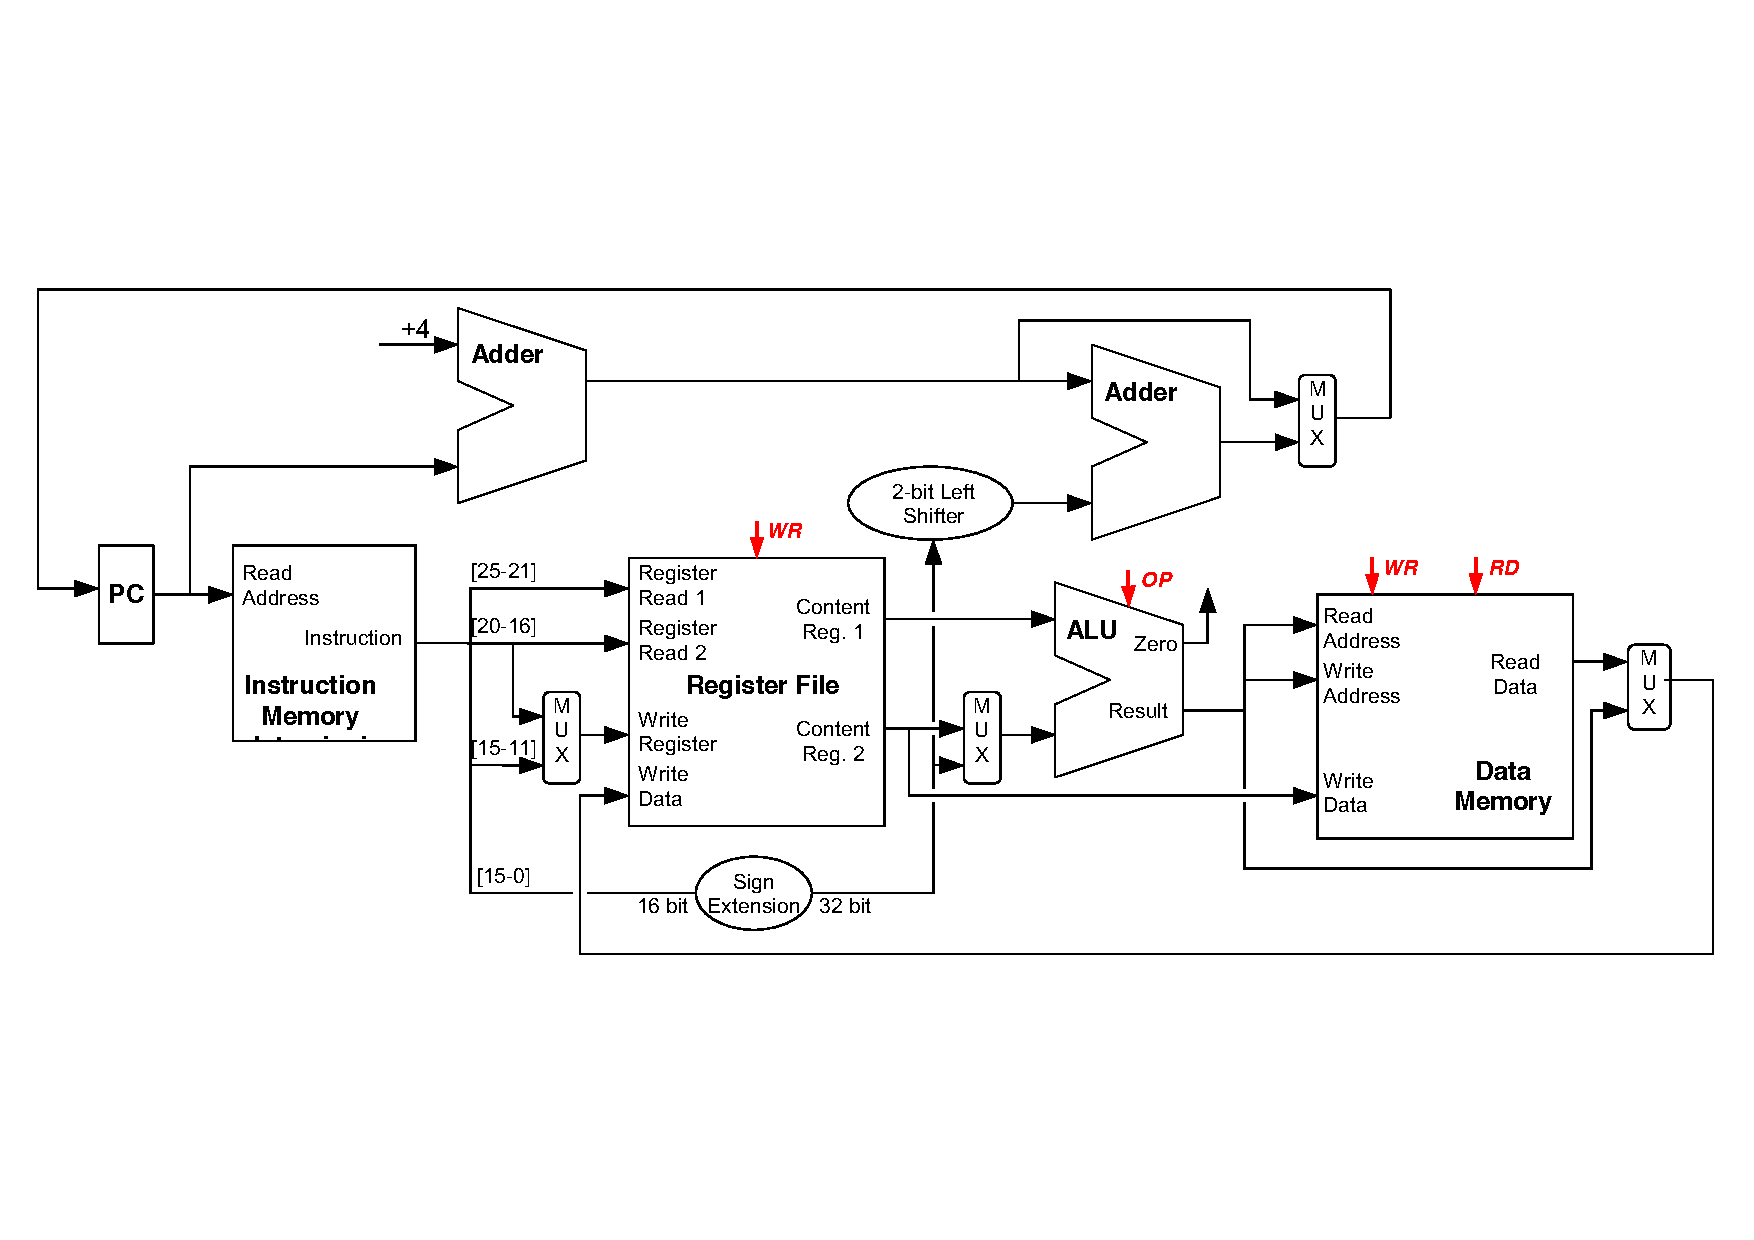
\includegraphics[width=\textwidth]{img/implementation-mips-datapath.pdf}
    \caption{An implementation of MIPS data path (no Control Unit).\cite{pipelining-slides}}
    \label{fig: implementation of MIPS data path (no Control Unit)}
\end{figure}

\newpage

\noindent
Scan (or click) the QR code below to view the figure~\ref{fig: implementation of MIPS data path (no Control Unit)} in high quality:
\begin{center}
    \qrcode{https://github.com/PoliMI-HPC-E-notes-projects-AndreVale69/HPC-E-PoliMI-university-notes/tree/main/advanced-computer-architectures/notes/img/implementation-mips-datapath.pdf}
\end{center}

\begin{figure}[!htp]
    \centering
    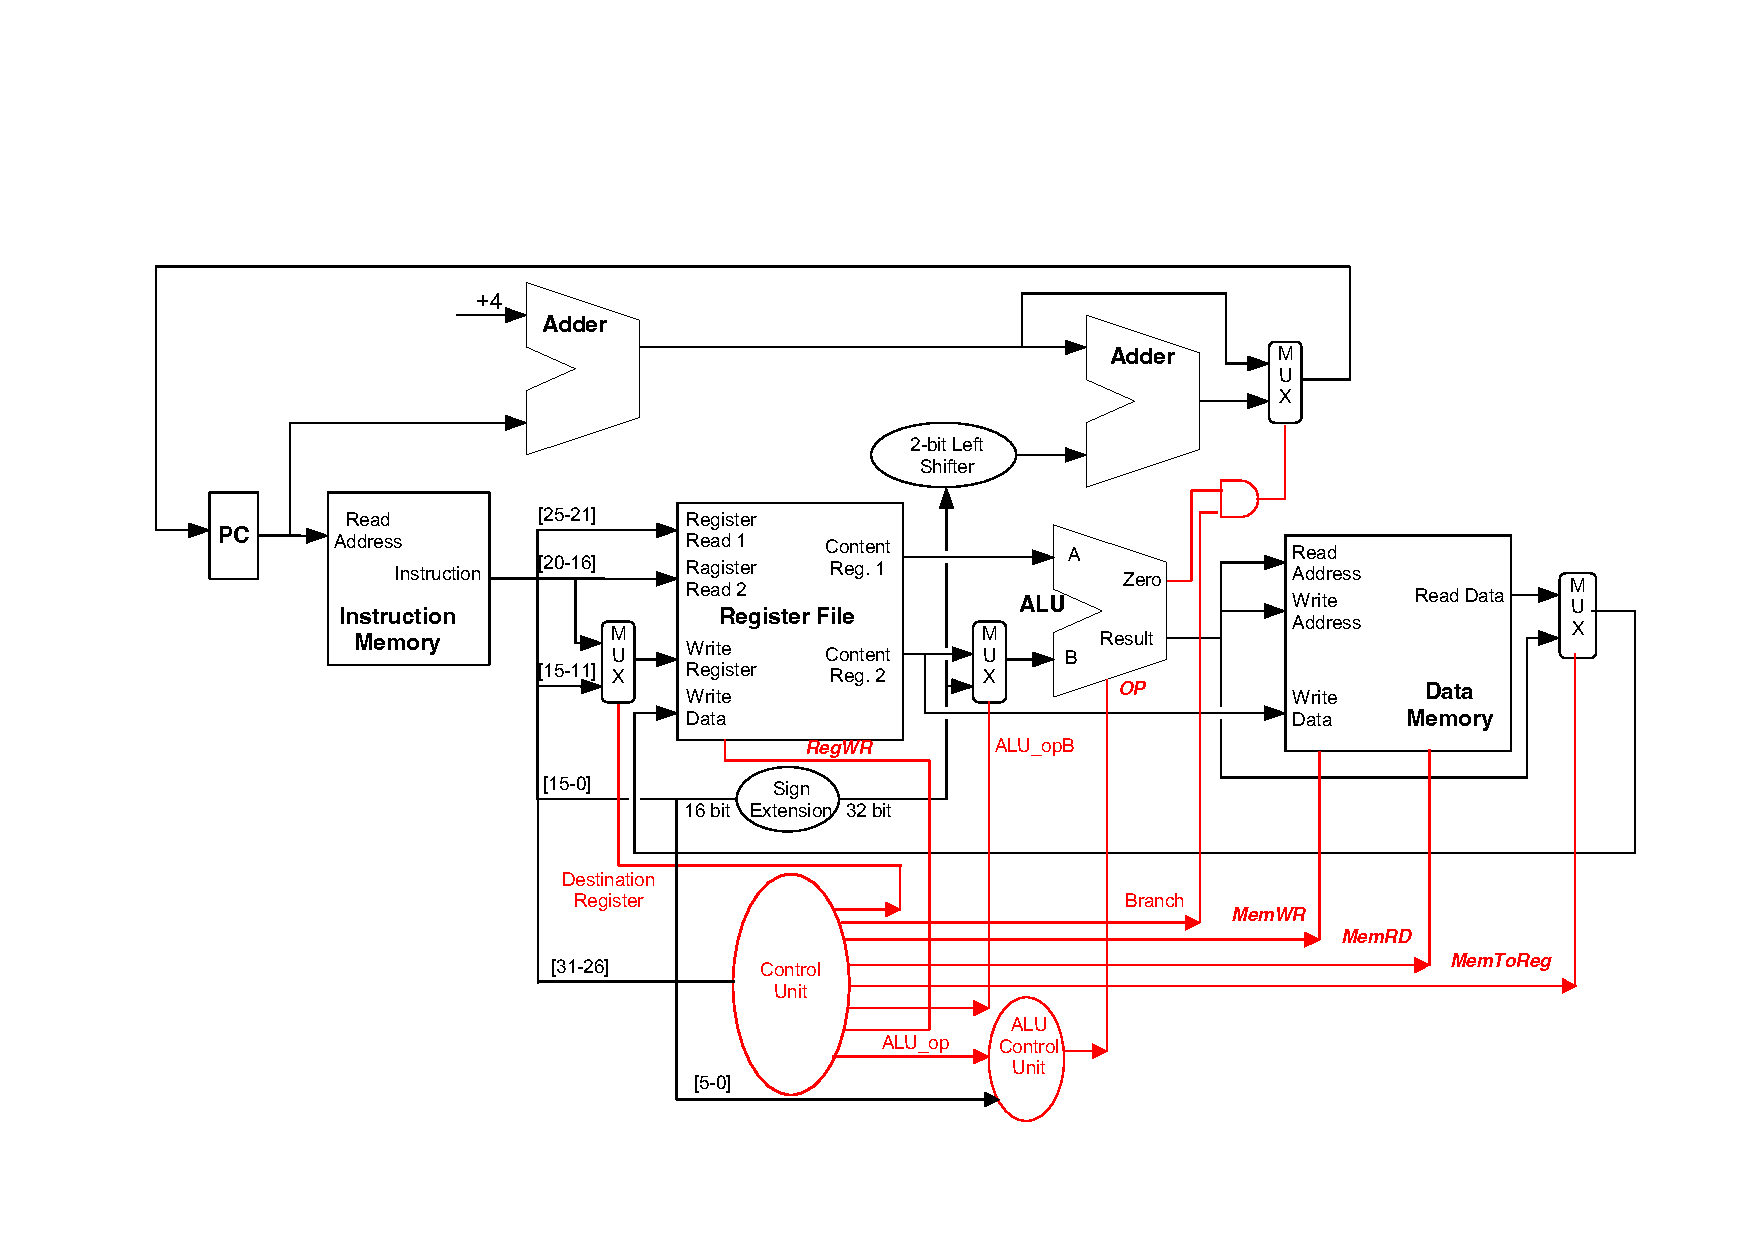
\includegraphics[width=\textwidth]{img/implementation-mips-datapath-cu.pdf}
    \caption{A complete implementation of MIPS data path.\cite{pipelining-slides}}
    \label{fig: complete implementation of MIPS data path}
\end{figure}

\noindent
Scan (or click) the QR code below to view the figure~\ref{fig: complete implementation of MIPS data path} in high quality:
\begin{center}
    \qrcode{https://github.com/PoliMI-HPC-E-notes-projects-AndreVale69/HPC-E-PoliMI-university-notes/tree/main/advanced-computer-architectures/notes/img/implementation-mips-datapath-cu.pdf}
\end{center}
    \subsubsection{MIPS Pipelining}

In simple words, the Instruction Pipelining (or Pipelining) is a technique for implementing instruction-level parallelism within a single processor. Pipelining attempts to keep every part of the processor busy with some instruction by dividing incoming instructions into a series of sequential steps (the eponymous \dquotes{pipeline}) performed by different processor units with different parts of instructions processed in parallel.

\highspace
\begin{definitionbox}
    \definition{Pipelining} is a performance optimization technique based on the \textbf{overlap} of the execution of multiple instructions deriving from a sequential execution flow.
\end{definitionbox}

\noindent
Pipelining exploits the \textbf{parallelism among instructions in a sequential instruction stream}.

\begin{flushleft}
    \textcolor{Red2}{\faIcon[regular]{star} \textbf{Basic idea}}
\end{flushleft}
The execution of an \textbf{instruction is divided into different phases} (called \definition{pipelines stages}), requiring a fraction of the time necessary to complete the instruction. These stages are connected one to the next to form the pipeline: 
\begin{enumerate}
    \item Instructions enter the pipeline at one end;
    \item Progress through the stages;
    \item And exit from the other end.
\end{enumerate}
As in the assembly line.

\begin{flushleft}
    \textcolor{Green3}{\faIcon{check} \textbf{Advantage}}
\end{flushleft}
The \textbf{Pipelining is transparent for the programmer}. To understand what it means, let's make an example.

\begin{examplebox}
    Image a car assembly line (e.g. Ferrari). A new car exits from the Ferrari assembly line in the time necessary to complete one of the phases. The pipelining technique doesn't reduce the time required to complete a car (the \textbf{latency}), BUT increases the number of vehicles produced per time unit (the \textbf{throughput}) and the frequency to complete cars.
\end{examplebox}

\newpage

\begin{examplebox}
    Image a sequential laundry jobs over time:\cite{pipelining-slides}
    \begin{center}
        \centering
        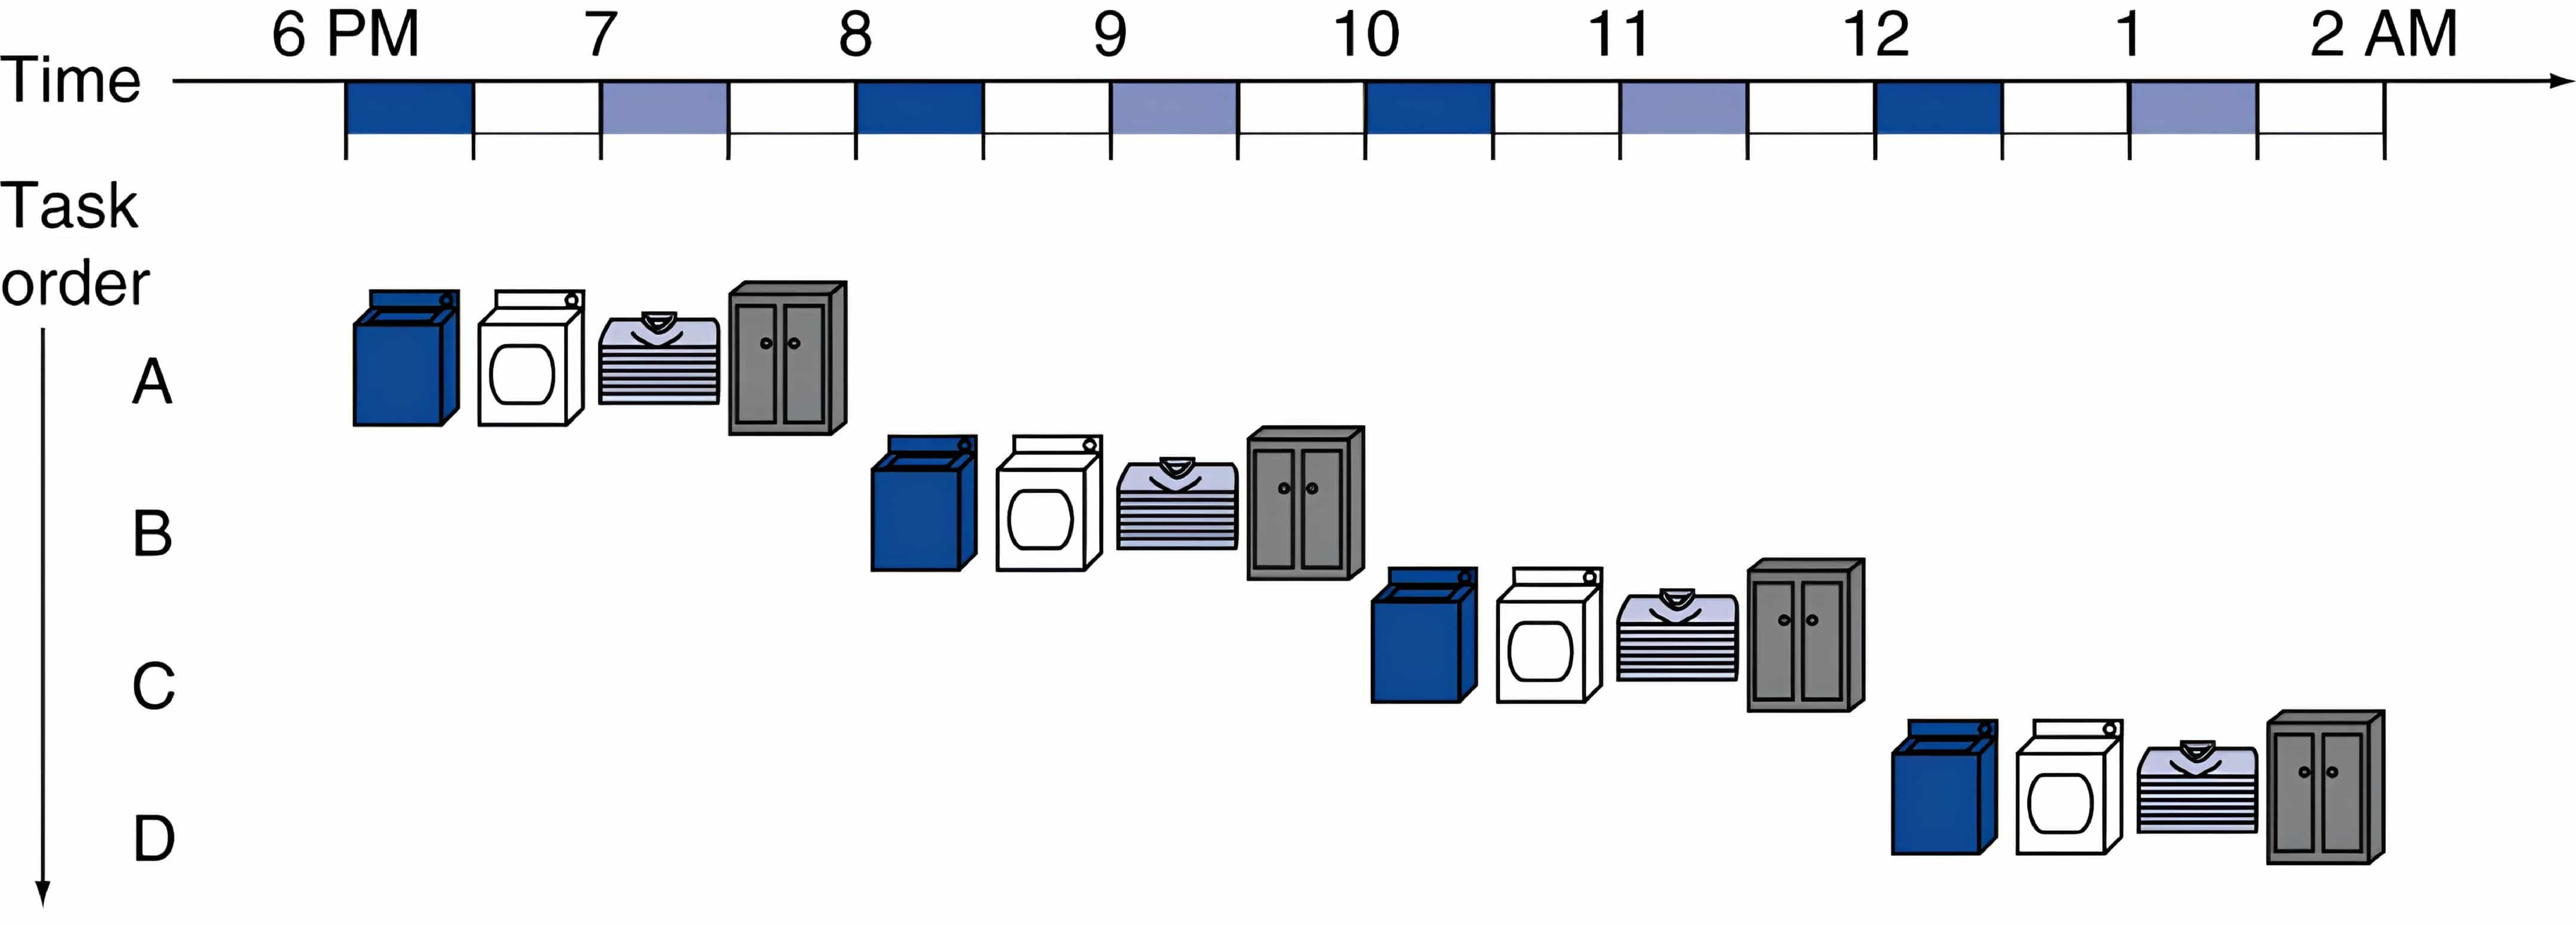
\includegraphics[width=.9\textwidth]{img/pipelining-example-1.pdf}
    \end{center}
    The pipelined laundry. Overlapping execution of stages to improve throughput (number of jobs executed per hour):\cite{pipelining-slides}
    \begin{center}
        \centering
        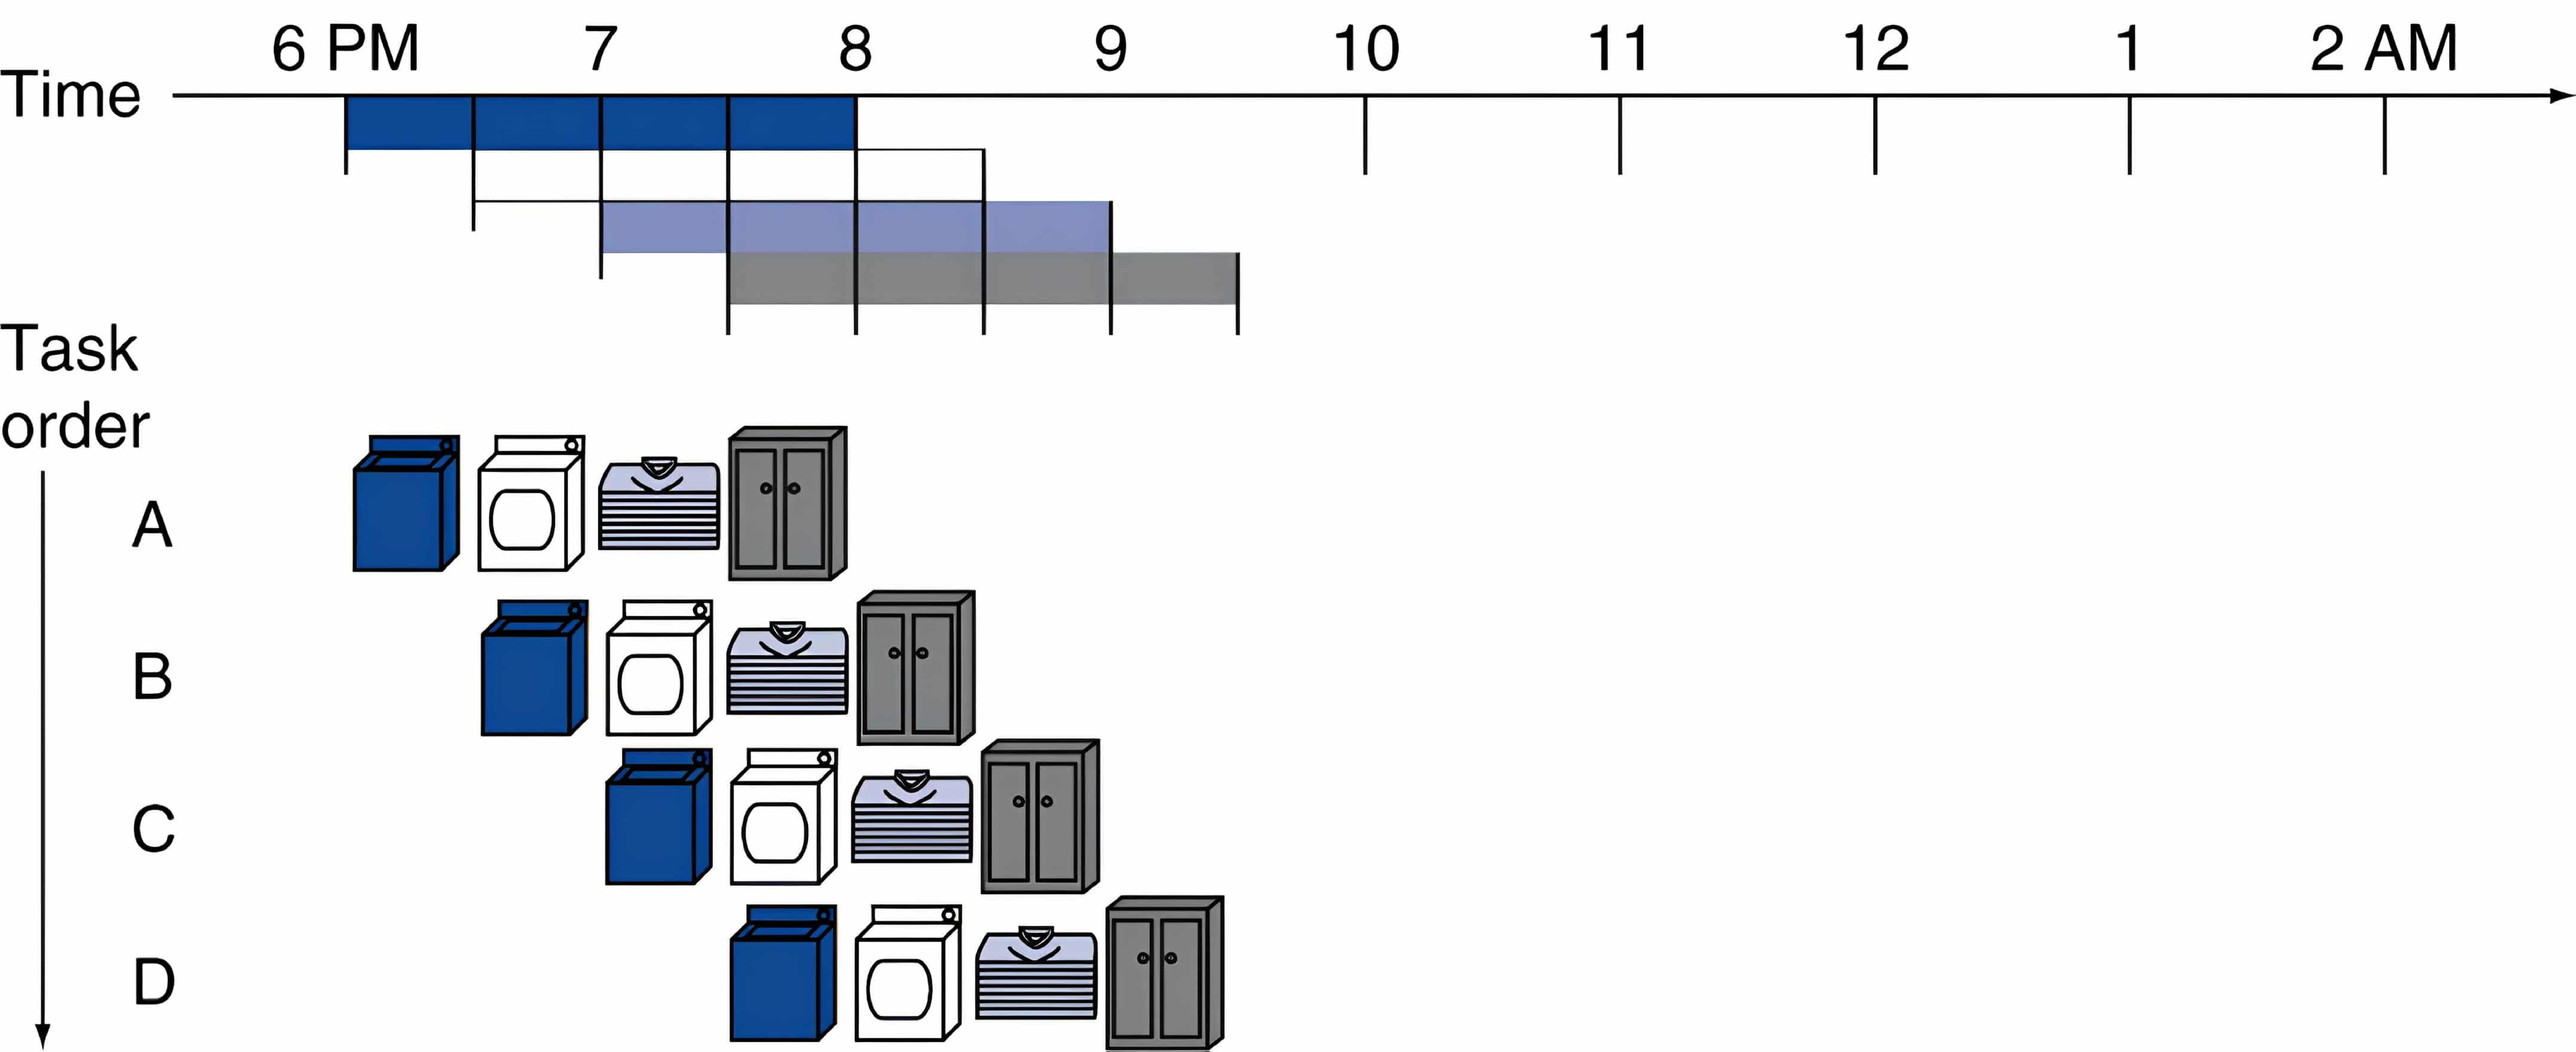
\includegraphics[width=.9\textwidth]{img/pipelining-example-2.pdf}
    \end{center}
\end{examplebox}

\noindent
As introduced in the previous example, sequential execution is slower than pipelining. The following figure shows the difference (in terms of clock cycles) between sequential and pipelining.
\begin{figure}[!htp]
    \centering
    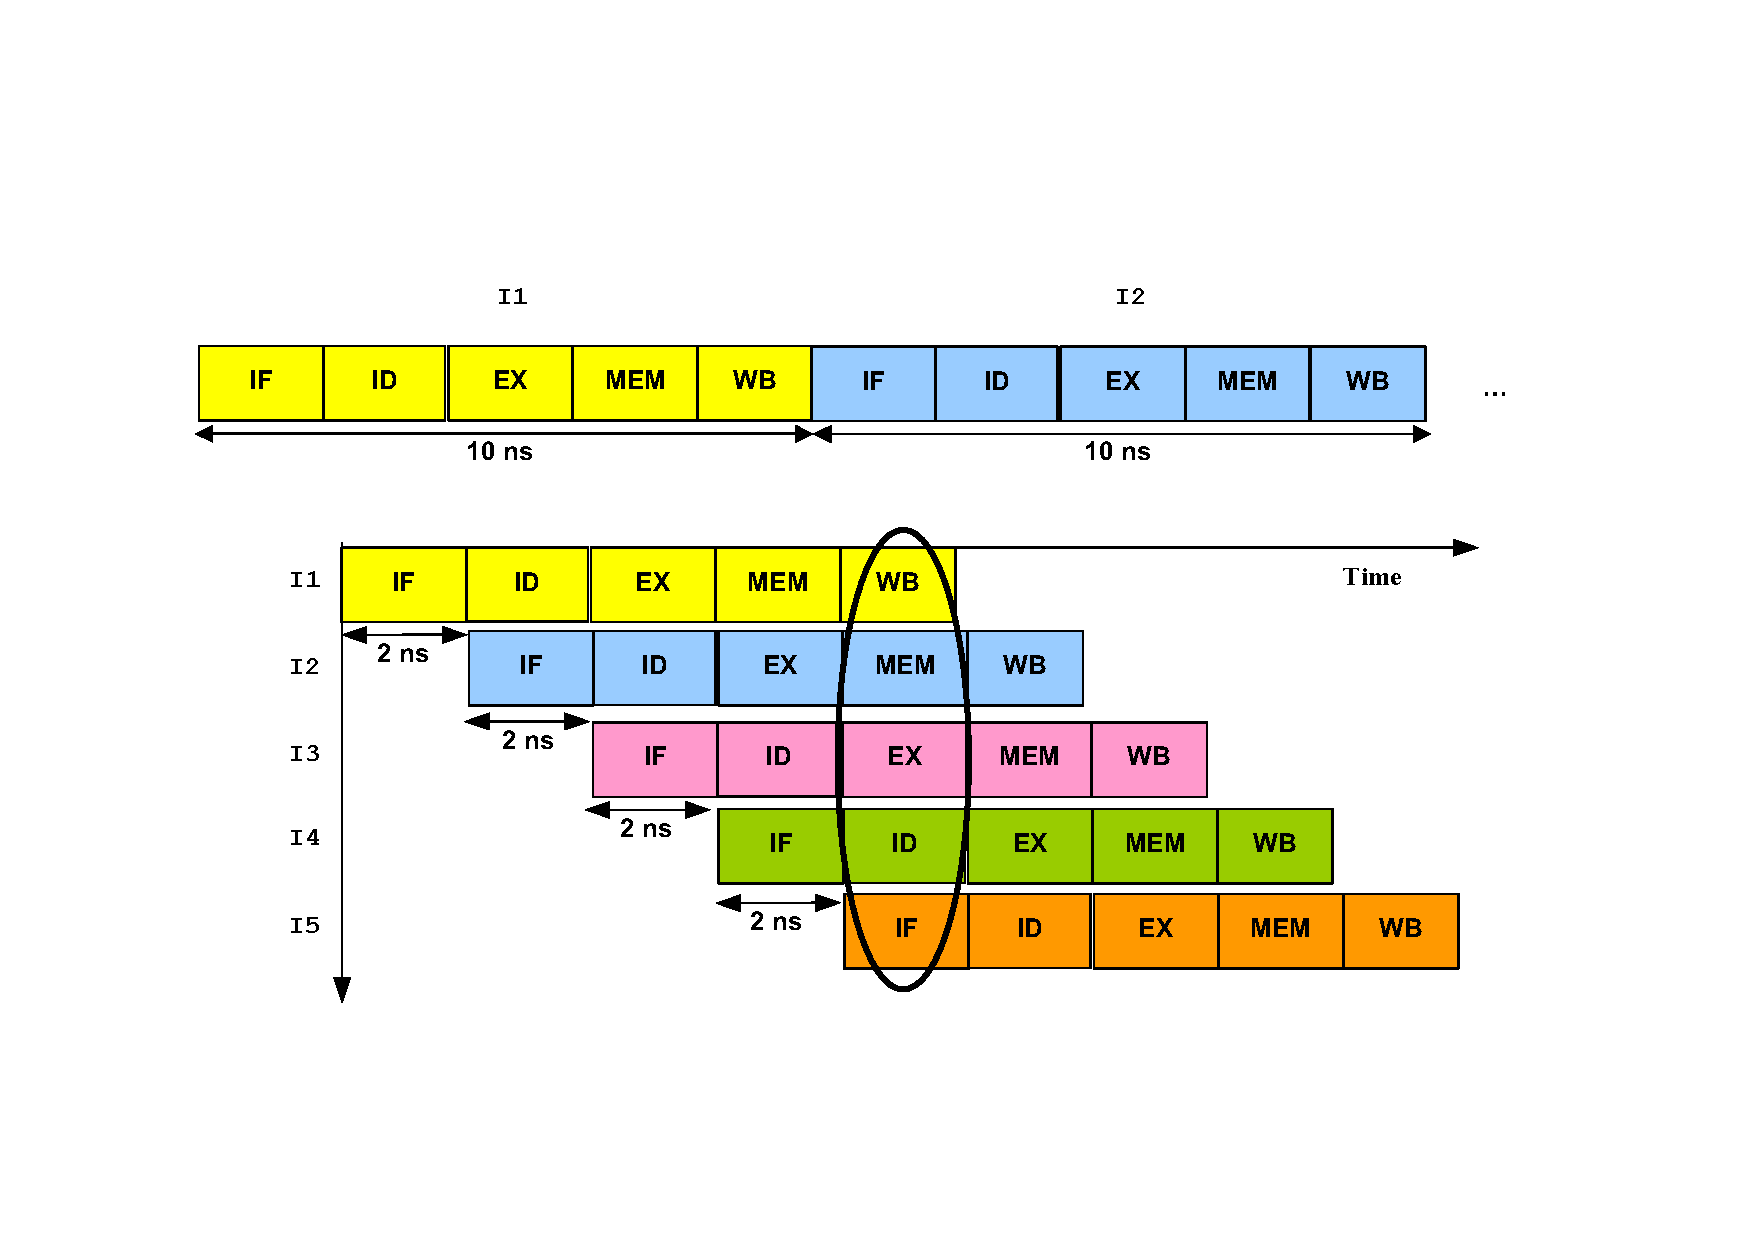
\includegraphics[width=\textwidth]{img/sequential-vs-pipelining-1.pdf}
    \caption{Sequential vs Pipelining.\cite{pipelining-slides}}
    \label{fig: sequential vs pipelining}
\end{figure}

\newpage

\noindent
The time to advance the instruction of one stage in the pipeline corresponds to a clock cycle. So the total cost is: 9 clock cycles.

\highspace
It's obvious that the \textbf{pipeline stages must be synchronized}: the duration of a clock cycle is defined by the time required by the slower stage in the pipeline (i.e. 2 ns). The \textbf{main goal} is to \textbf{balance the length of each pipeline stage}. If the stages are perfectly balanced, the \textbf{ideal speedup} due to pipelining is equal to the number of pipeline stages.

\begin{definitionbox}
    The \definition{ideal speedup} must be the \textbf{same value of the pipeline stages}.
\end{definitionbox}

\highspace
Look again at Figure~\ref{fig: sequential vs pipelining}. The sequential and pipelining cases consist of 5 instructions, each of which is divided into 5 low-level instructions of 2 ns each.
\begin{itemize}
    \item The \textbf{latency} (total execution time) of each instruction is not varied, it's always 10 ns.
    \begin{definitionbox}
        The \definition{latency} is the execution time of a single instruction.
    \end{definitionbox}

    \item The \textbf{throughput} (number of low-level instructions completed in the time unit) is improved:
    \begin{itemize}
        \item Sequential: 5 instructions in 50 ns (1 instruction per 10 ns, $50 \div 5 = 10$)
        \item Pipelining: 5 instruction in 18 ns (1 instruction per 3.6 ns, $18 \div 5 = 3.6$)
    \end{itemize}
    \begin{definitionbox}
        The \definition{throughput} is the number of instructions completed per unit of time.
    \end{definitionbox}
\end{itemize}

\newpage

\begin{center}
    \large
    \textcolor{Red3}{\textbf{Pipeline Execution of MIPS Instructions}}
\end{center}
On page~\pageref{Execution (EX) details} we discussed some MIPS instructions to understand how the MIPS architecture works. The aim of the following pages is to understand \textbf{how MIPS works in a pipelined execution}.

\highspace
We want to perform the following assembly lines:
\lstinputlisting[language=misc]{code/mips-pipelining/sequential-vs-pipelining.s}
\begin{figure}[!htp]
    \centering
    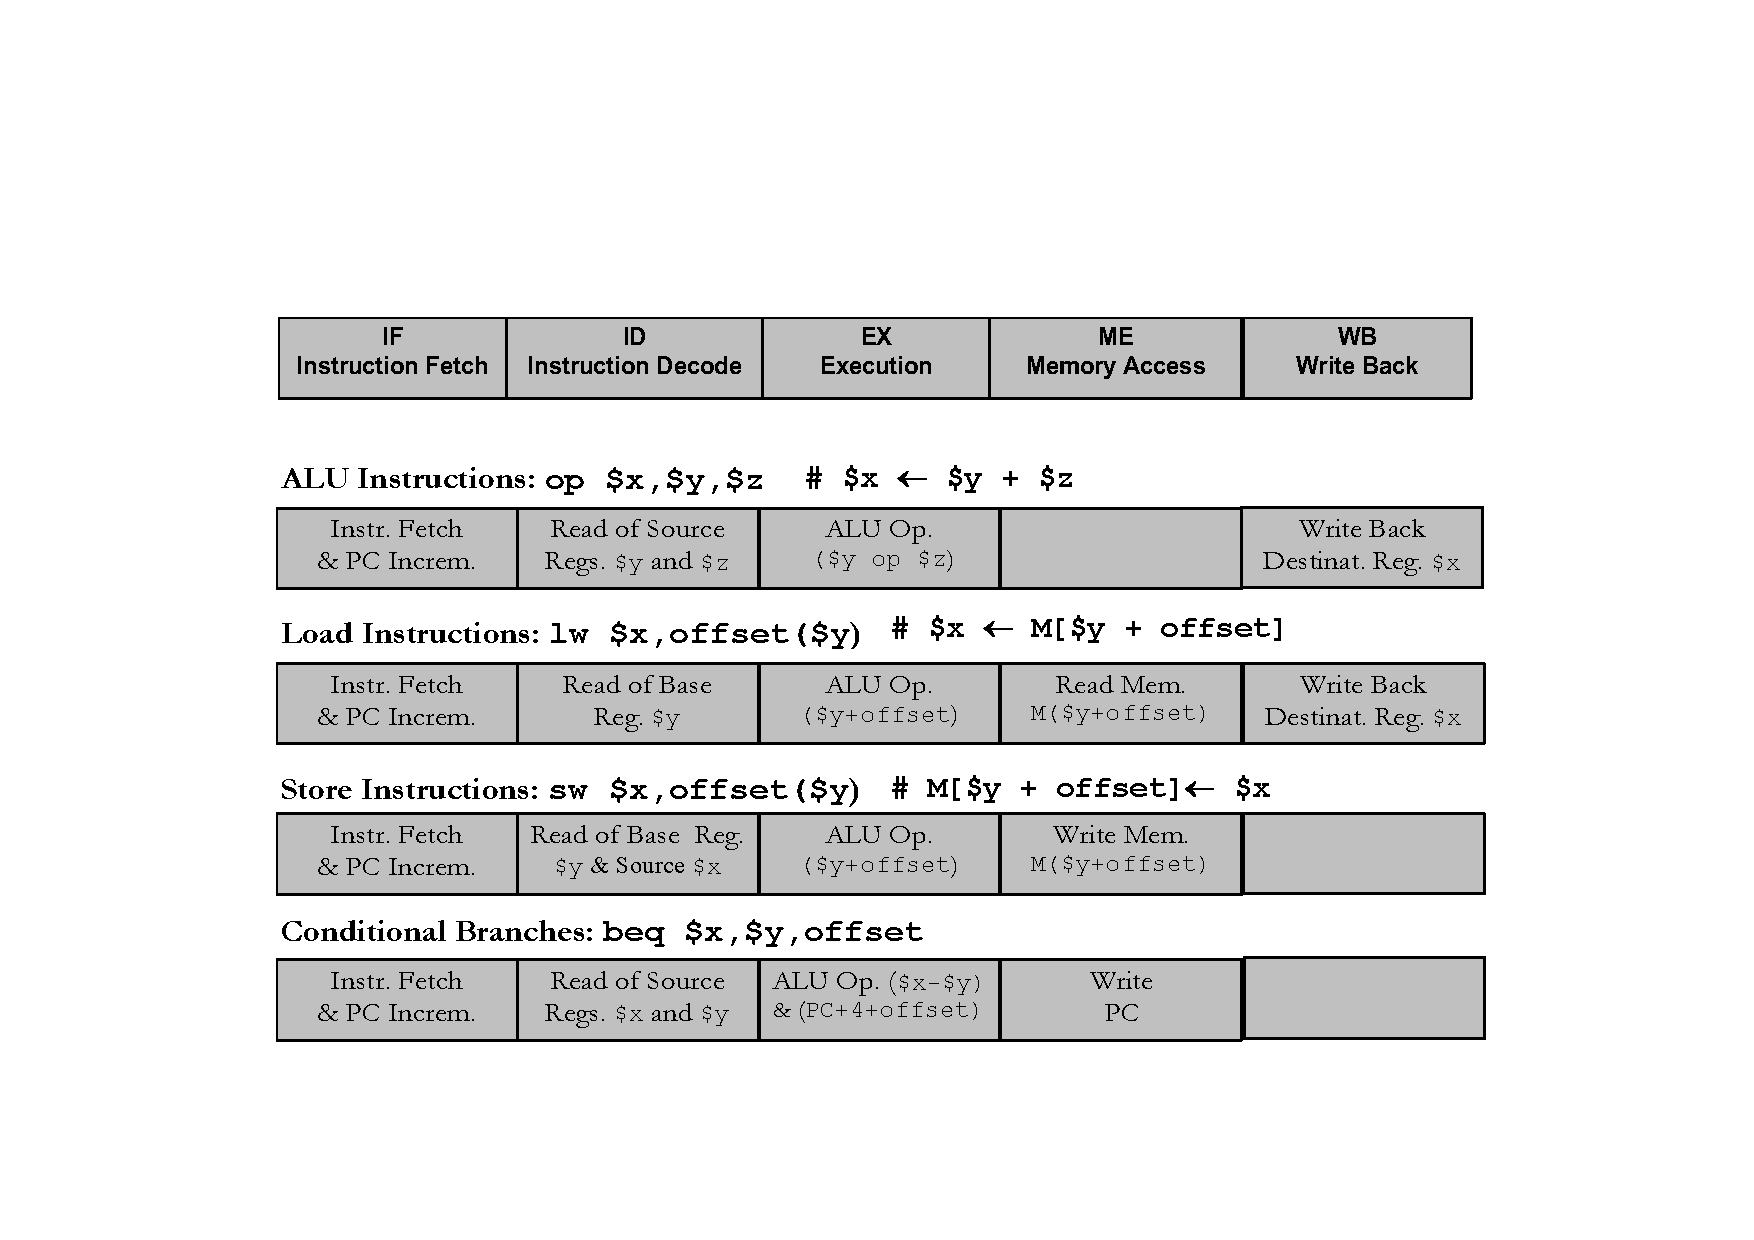
\includegraphics[width=\textwidth]{img/sequential-vs-pipelining-2.pdf}
    \caption{Pipeline Execution of MIPS Instructions.\cite{pipelining-slides}}
\end{figure}

\newpage

\begin{center}
    \textcolor{Red3}{\textbf{Resources used during the pipeline execution}}
\end{center}
\begin{figure}[!htp]
    \centering
    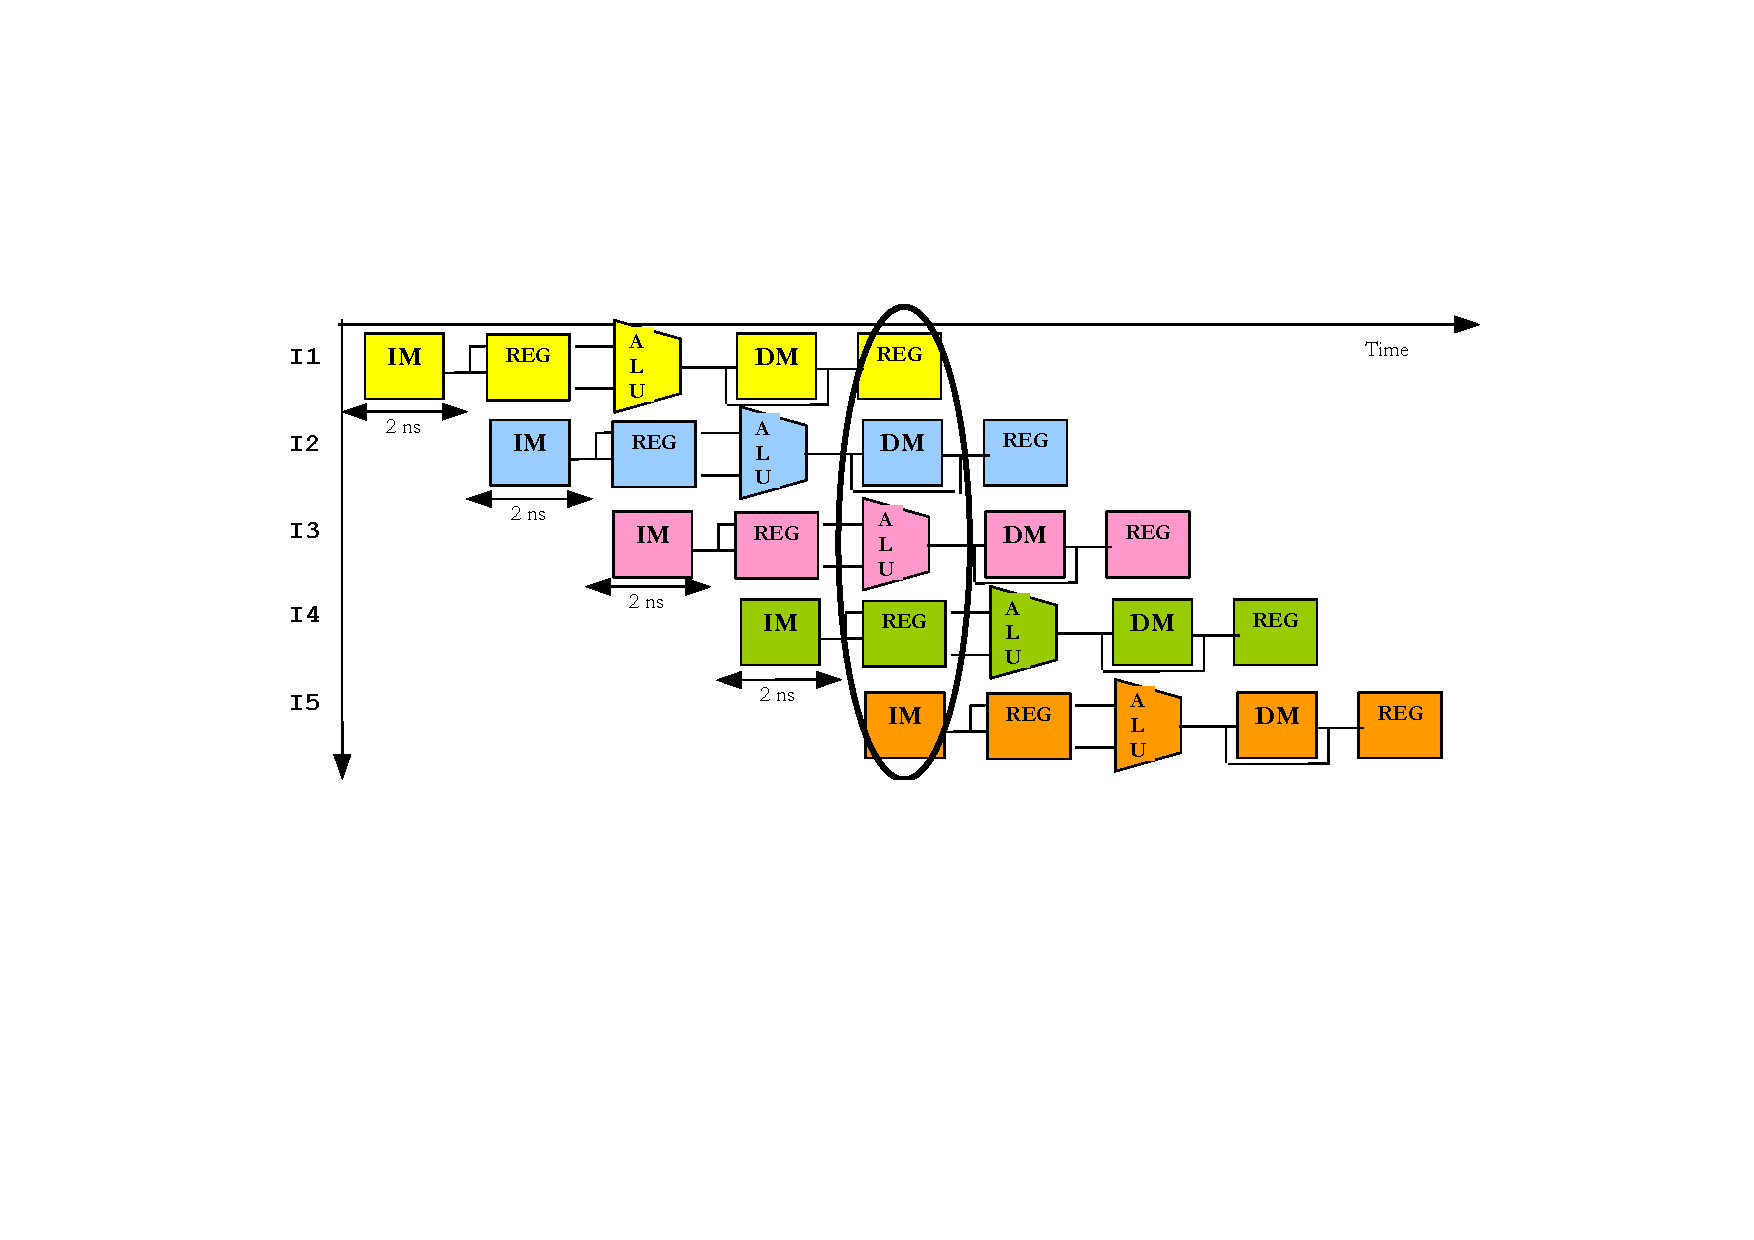
\includegraphics[width=\textwidth]{img/sequential-vs-pipelining-3.pdf}
    \caption{Resources used during the pipeline execution (IM is Instruction Memory, REG is Register File and DM is Data Memory).\cite{pipelining-slides}}
\end{figure}

\newpage

\begin{center}
    \large
    \textcolor{Red3}{\textbf{Implementation of MIPS pipeline}}
\end{center}
The division of the execution of each instruction in $n$ stages implies that in each clock cycle, there are $n$ instructions for execution. That means the CPU must have $n$ modules corresponding to $n$ execution stages. Therefore, to do pipelining, we need \definition{pipeline registers} \textbf{to separate the different stages}.

\highspace
In the following figure, we can see how the pipeline registers are implemented. Between each phase of execution of MIPS instructions (details on page \pageref{Phases of execution of MIPS Instructions}), there is a pipeline register holding the result of the instruction.
\begin{figure}[!htp]
    \centering
    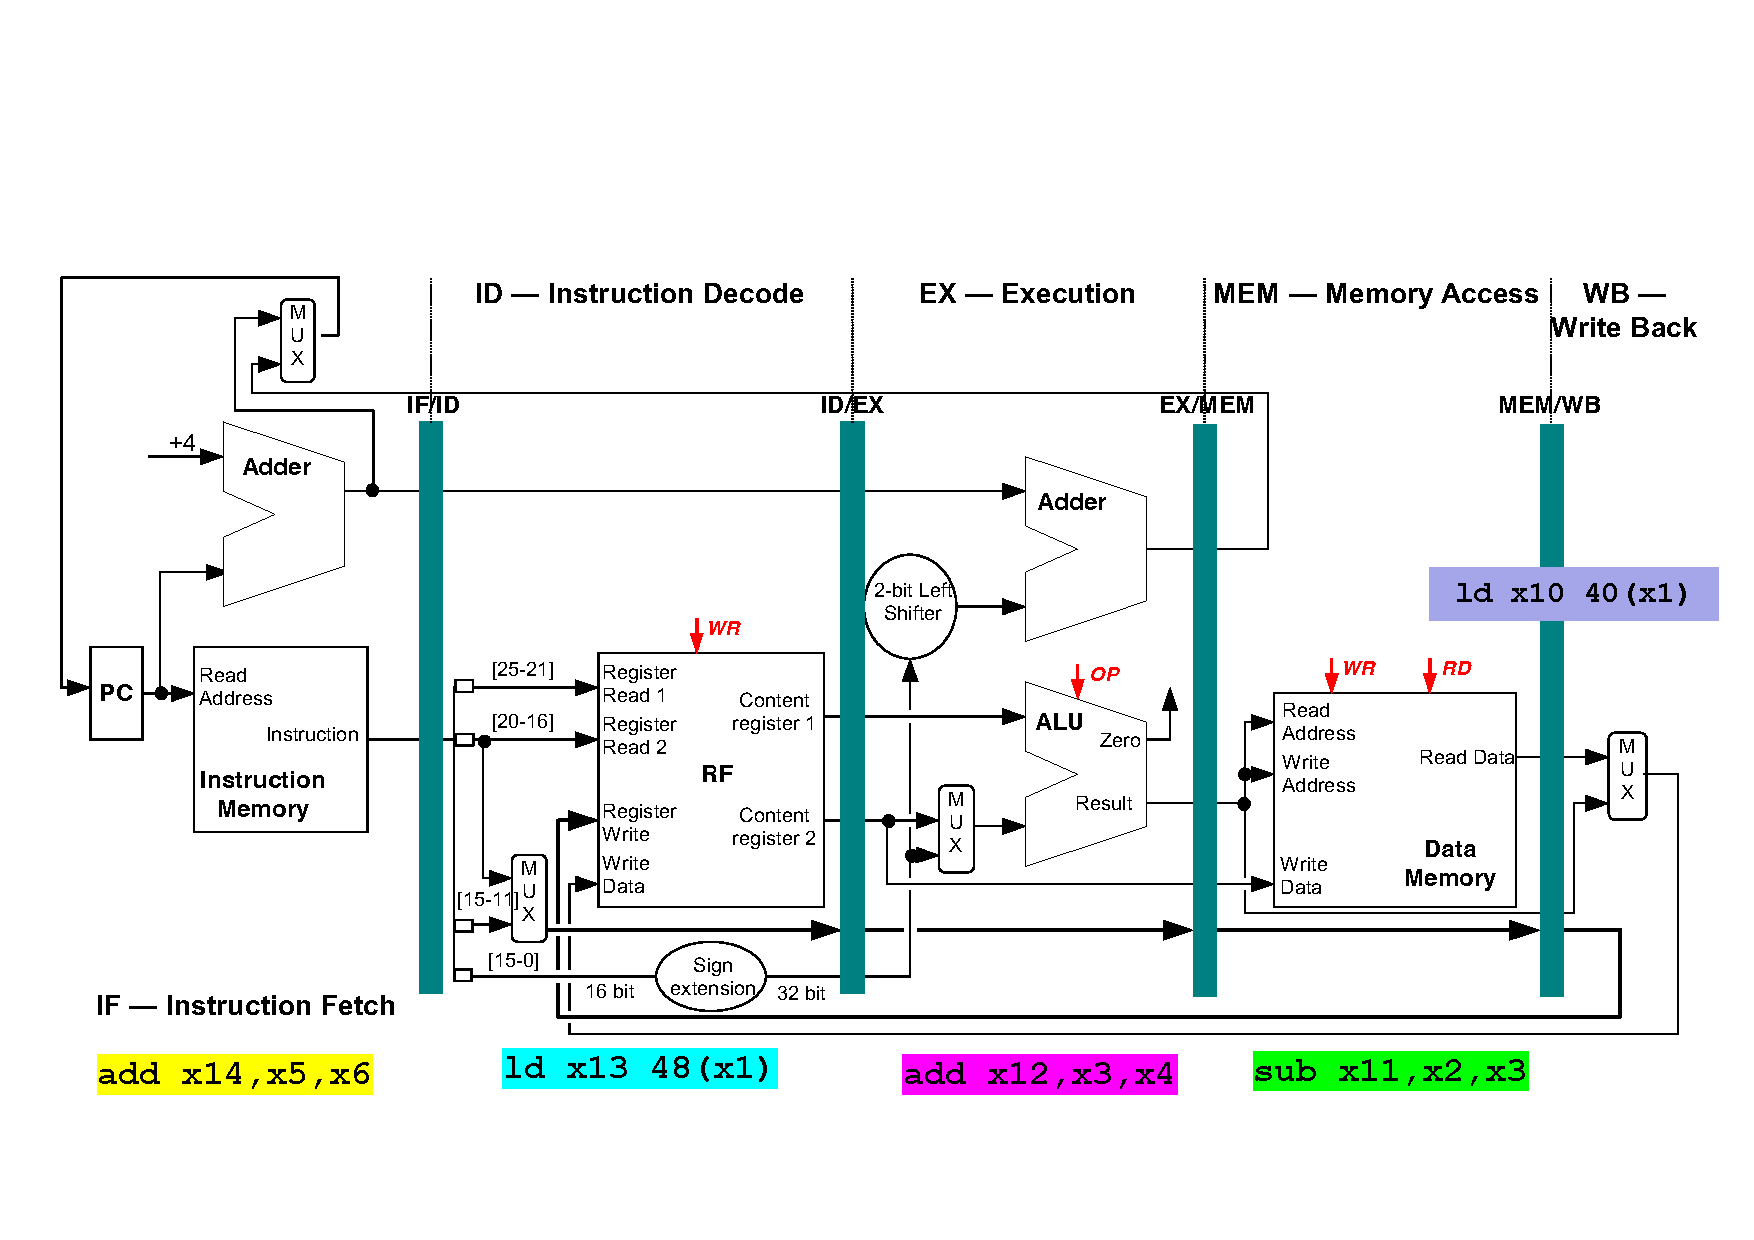
\includegraphics[width=\textwidth]{img/pipeline-registers-1.pdf}
    \caption{MIPS pipeline implementation.\cite{pipelining-slides}}
\end{figure}

\noindent
\underline{Note}: \textbf{the data stored in the interstage registers correspond (obviously) to different instructions}.

\newpage

\noindent
Finally, in the following figure we can see the timeline implementation of the pipeline registers. But there are two basic assumptions to make:
\begin{enumerate}
    \item There are no data dependencies between instructions. If there were, an instruction could read a register with an unknown value (Pipeline Hazard, page~\pageref{subsubsection: The problem of Pipeline Hazards}).

    \item There are no branch/jump instructions.
\end{enumerate}
\begin{figure}[!htp]
    \centering
    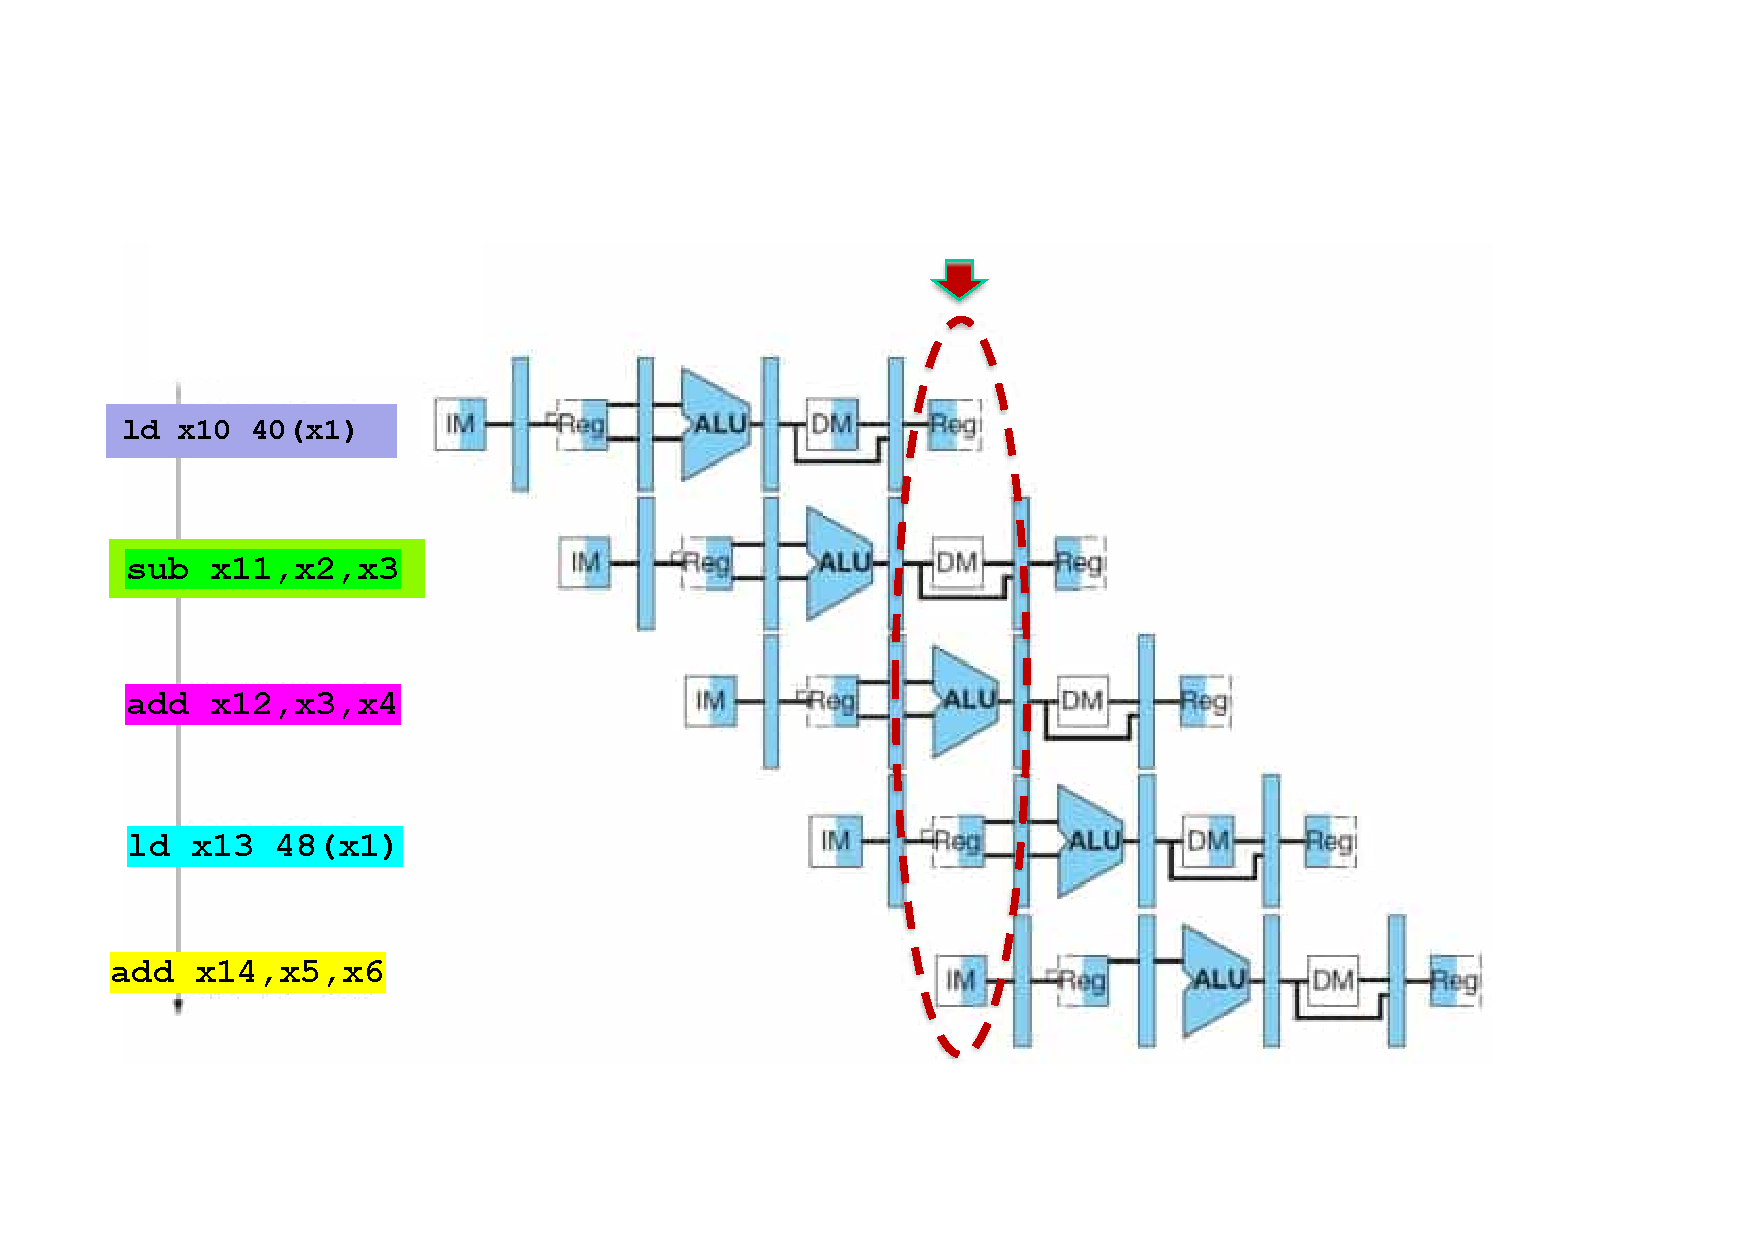
\includegraphics[width=\textwidth]{img/pipeline-registers-2.pdf}
    \caption{Timeline of MIPS pipeline implementation.\cite{pipelining-slides}}
\end{figure}
    \subsubsection{The problem of Pipeline Hazards}\label{subsubsection: The problem of Pipeline Hazards}

\begin{definitionbox}[: Hazard]
    A \definition{hazard (conflict)} is created whenever there a \textbf{dependence} between two instructions, and instructions are close enough that the overlap caused by pipelining would change the order of access to the operands involved in the dependence.
\end{definitionbox}

\begin{flushleft}
    \textcolor{Red2}{\faIcon{exclamation-triangle} \textbf{Problem Consequences}}
\end{flushleft}
The Hazards:
\begin{itemize}
    \item \textbf{Force} the next \textbf{instruction} in the pipeline \textbf{to be executed later} than its intended clock cycle.

    \item \textbf{Reduced the performance} from the ideal speedup achieved by pipelining (direct previous consequence).
\end{itemize}
There are \textbf{three classes} of Hazards:
\begin{itemize}
    \item \definition{Structural Hazards}. Attempt to use the \textbf{same resource from different instructions simultaneously}.
    
    \example{Example}: single memory for instruction and data.
    

    \item \definition{Data Hazards}. Attempt to \textbf{use a result before it is ready}.
    
    \example{Example}: instruction depending on a result of a previous instruction still in the pipeline.

    There are also \textbf{two specific forms} of data hazard, called \definition{Load-Use Data Hazard} and \definition{Load-Store Data Hazard}. Both occur when the \textbf{data loaded by a load instruction is not yet available when it is needed by another instruction}. In the case of Load-Use, the \dquotes{another instruction} is an operator such as \texttt{add}; in the case of Load-Store, the \dquotes{another instruction} is the store (\texttt{sw}) instruction.

    The following \example{example} shows the conflict (Load-Use Data Hazard) between two instructions. In particular, the value \texttt{lw} writes to \texttt{s2} is not available until \texttt{lw} has completed the \texttt{MEM} phase, but \texttt{and} needs this value when it enters the \texttt{EX} phase, i.e. when \texttt{lw} enters the \texttt{MEM} phase.
    \lstinputlisting[language=misc]{code/the-problem-of-pipeline-hazards/load-use-data-hazard.s}

    \item \definition{Control Hazards}. Attempt to \textbf{make a decision on the next instruction to execute before the condition is evaluated} (more detailed analysis on page \pageref{flushleft: how to detect Control Hazards}).
    
    \example{Example}: conditional branch execution.
\end{itemize}

\begin{flushleft}
    Structural Hazards? No problem for MIPS Architecture!
\end{flushleft}
\textbf{There aren't any structural hazards in MIPS architecture} because the Instruction Memory (IM) is separated from the Data Memory (DM). Also, the Register File (RF) is used in the same clock cycle (read access by an instruction and write access by another instruction).

\newpage

\begin{flushleft}
    \textcolor{Green3}{\faIcon{question-circle} \textbf{How to detect \underline{Data Hazards}? Dependency Analysis}}
\end{flushleft}
To \textbf{detect Data Hazards}, it is suggested to analyze the dependencies. If the instructions executed in the pipeline depend on each other, data hazards can arise \textbf{when instructions are too close}. For \example{example}:
\lstinputlisting[language=misc]{code/the-problem-of-pipeline-hazards/data-hazards-1.s}
Data Hazards can occur in a variety of situations, but a \textbf{true dependency situation} is created by a \textbf{RAW (Read After Write) Hazard}.

\begin{definitionbox}[: Read After Write Hazard]
    A \definition{RAW (Read After Write) Hazard} occurs when an instruction $n+1$ tries to read a source operand before the previous instruction $n$ has written its value in the Register File (RF).
\end{definitionbox}

\noindent
For \example{example}:
\lstinputlisting[language=misc]{code/the-problem-of-pipeline-hazards/RAW-hazard-1.s}

\newpage

\begin{flushleft}
    \textcolor{Green3}{\faIcon{question-circle} \textbf{How to detect \underline{Control Hazards}? Check conditional branches}}
    \label{flushleft: how to detect Control Hazards}
\end{flushleft}
First of all, some \example{examples} of conditional branches for MIPS processor are: \texttt{beq} (branch on equal) and \texttt{bne} (branch on not equal):
\lstinputlisting[language=misc]{code/mips-architecture/beq-bne.s}
The \textbf{address to which you want to branch} is called the \definition{Branch Target Address}. If the branch condition:
\begin{itemize}
    \item Is satisfied $\Rightarrow$ the \textbf{branch is taken} and the Branch Target Address is stored in the Program Counter (PC).

    \item Is \underline{not} satisfied $\Rightarrow$ the \textbf{branch is not taken} (untaken) and the instruction stream is executed sequentially with the next instruction address (PC $+ 4$).
\end{itemize}
In detail, the stages are the following:
\begin{enumerate}
    \item \texttt{[IF]} Instruction fetch and PC increment.
    \item \texttt{[ID]} Instruction Decode and Registers Read (e.g. \texttt{x} and \texttt{y})
    \item \texttt{[EX]} Compare registers (e.g. \texttt{x} and \texttt{y}) in the ALU to derive the Branch Outcome: taken or not taken. Also, computation of the Branch Target Address, so $\texttt{PC} + 4 + \texttt{offset}$
    \item \texttt{[ME]} The Branch Outcome is used to decide the next PC:
    \begin{itemize}
        \item Is satisfied $\Rightarrow$ \texttt{PC} take $\texttt{PC} + 4 + \texttt{offset}$
        \item Is \underline{not} satisfied $\Rightarrow$ \texttt{PC} take $\texttt{PC} + 4$
    \end{itemize}
\end{enumerate}
Let us now move on to a more interesting analysis. To understand when the Control Hazards occur, think about the Branch Outcome and the Branch Target Address. Both are ready at the end of the EX (execution) phase (so between pass number 3 and 4). Finally, branches are resolved when the Program Counter is updated at the end of the Memory Access stage (after pass number 4). 

\highspace
To feed the condition branch into the pipeline, we need to \textbf{create a way where the condition branch is decided before the EX stage of the next instruction}. It's obvious, because if the Branch Outcome is positive, we need to skip the next instruction and do the conditional jump instead.

\highspace
This is a more detailed explanation of a control hazard. Control Hazards arise from the pipelining of conditional branches and other \texttt{jump} \textbf{instructions that change the PC}. They also \textbf{reduce the performance from the ideal speedup gained by pipelining}, because it is necessary to hold the pipeline until the branch is resolved.

\newpage

\begin{center}
    \large
    \textcolor{Red3}{\textbf{MIPS Optimized Pipeline}}
\end{center}
Consider the following situation:
\begin{figure}[!htp]
    \centering
    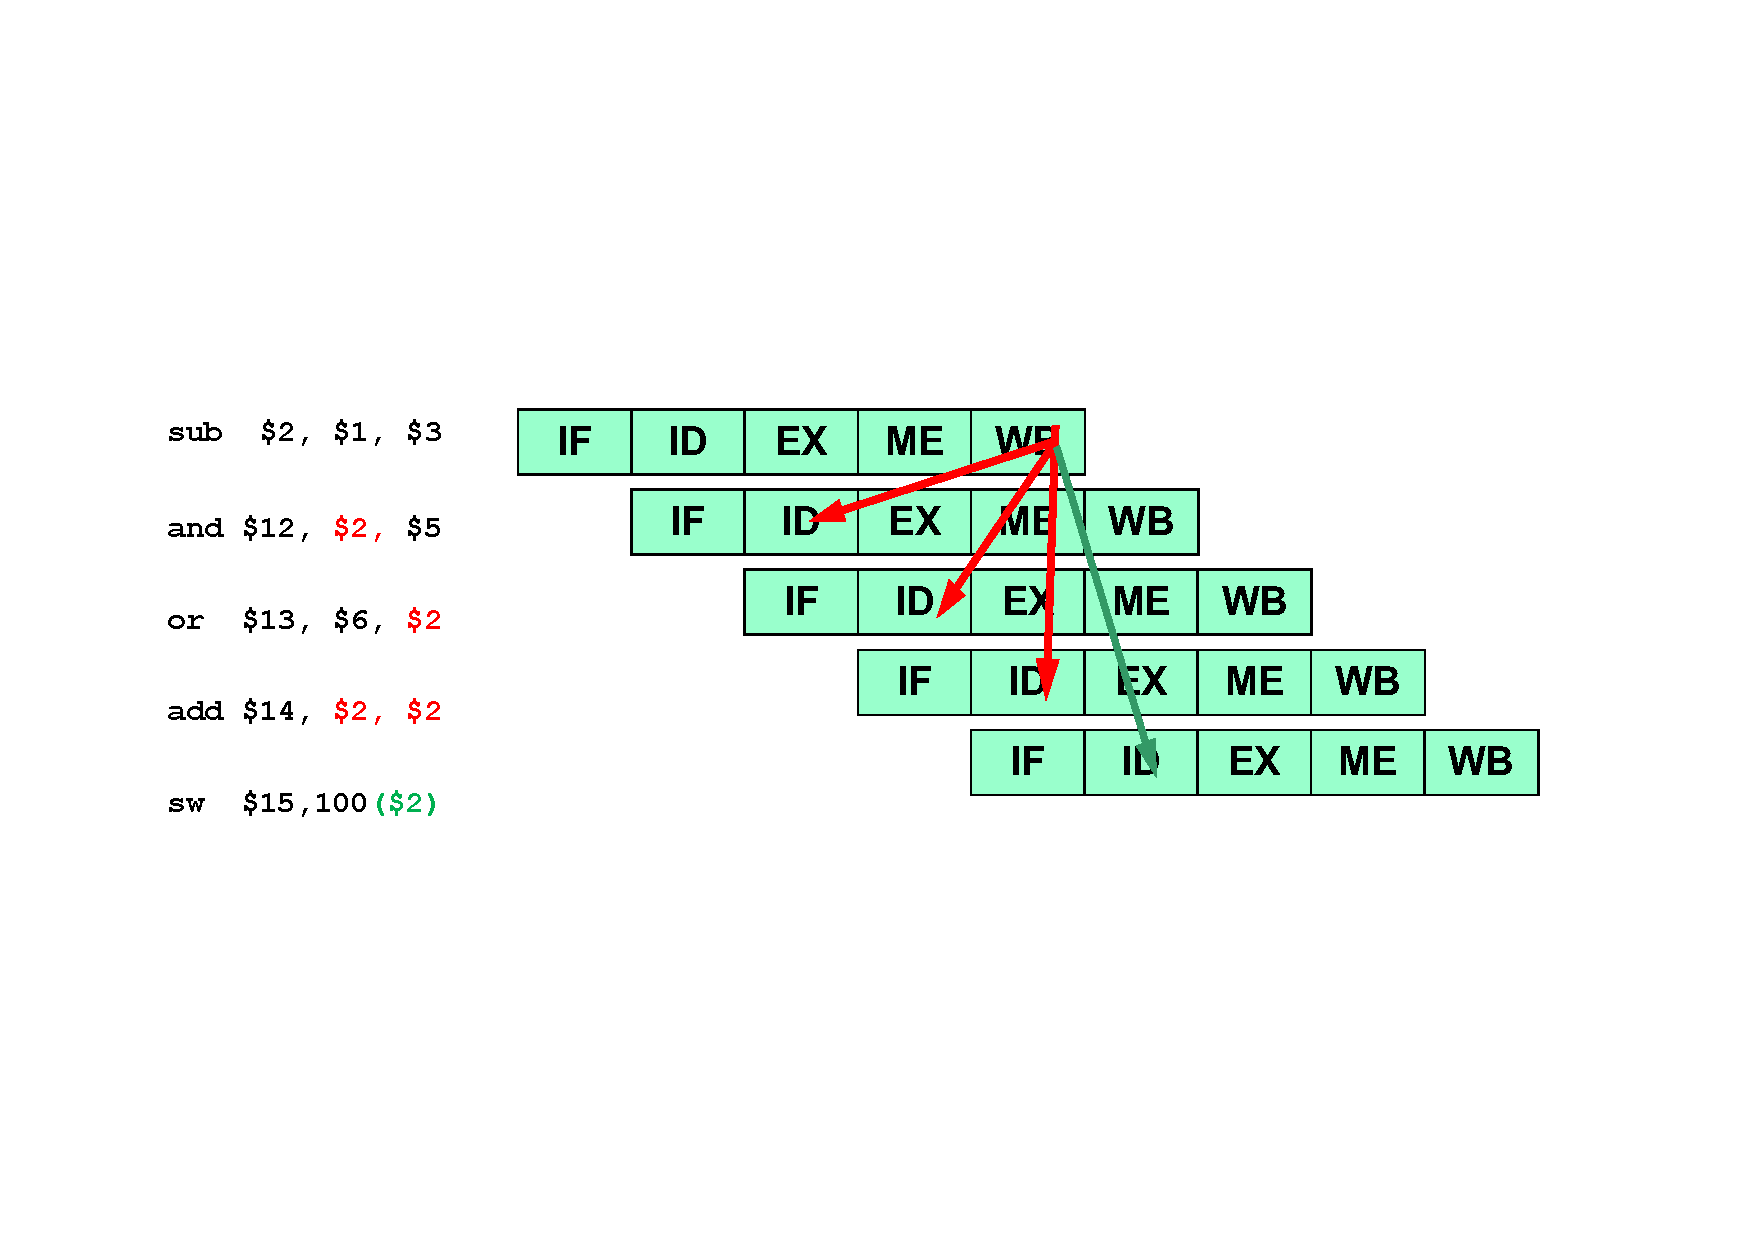
\includegraphics[width=\textwidth]{img/RAW-hazards-1.pdf}
    \caption{Why MIPS Optimized Pipeline was born.\cite{pipelining-slides}}
\end{figure}

\noindent
The Register File is used in 2 stages: read access during ID (\texttt{and} operation) and write access during Write Back (WB) (\texttt{sub} operation). \emph{What happens if read and write refer to the same register in the same clock cycle?} Or we insert a stall, or we use an \textbf{optimized pipeline} (smart choice).

\begin{definitionbox}[: Optimized Pipeline]
    By selecting \definition{Optimized Pipeline}, we assume the Register File (RF) read occurs in the second half of clock cycle and the Register File write in the first half of clock cycle.
\end{definitionbox}

\noindent
This way \textbf{we don't need the stall}. The following Figure~\ref{fig: Optimized Pipeline} shows an optimized pipeline.

\newpage

\begin{figure}[!htp]
    \centering
    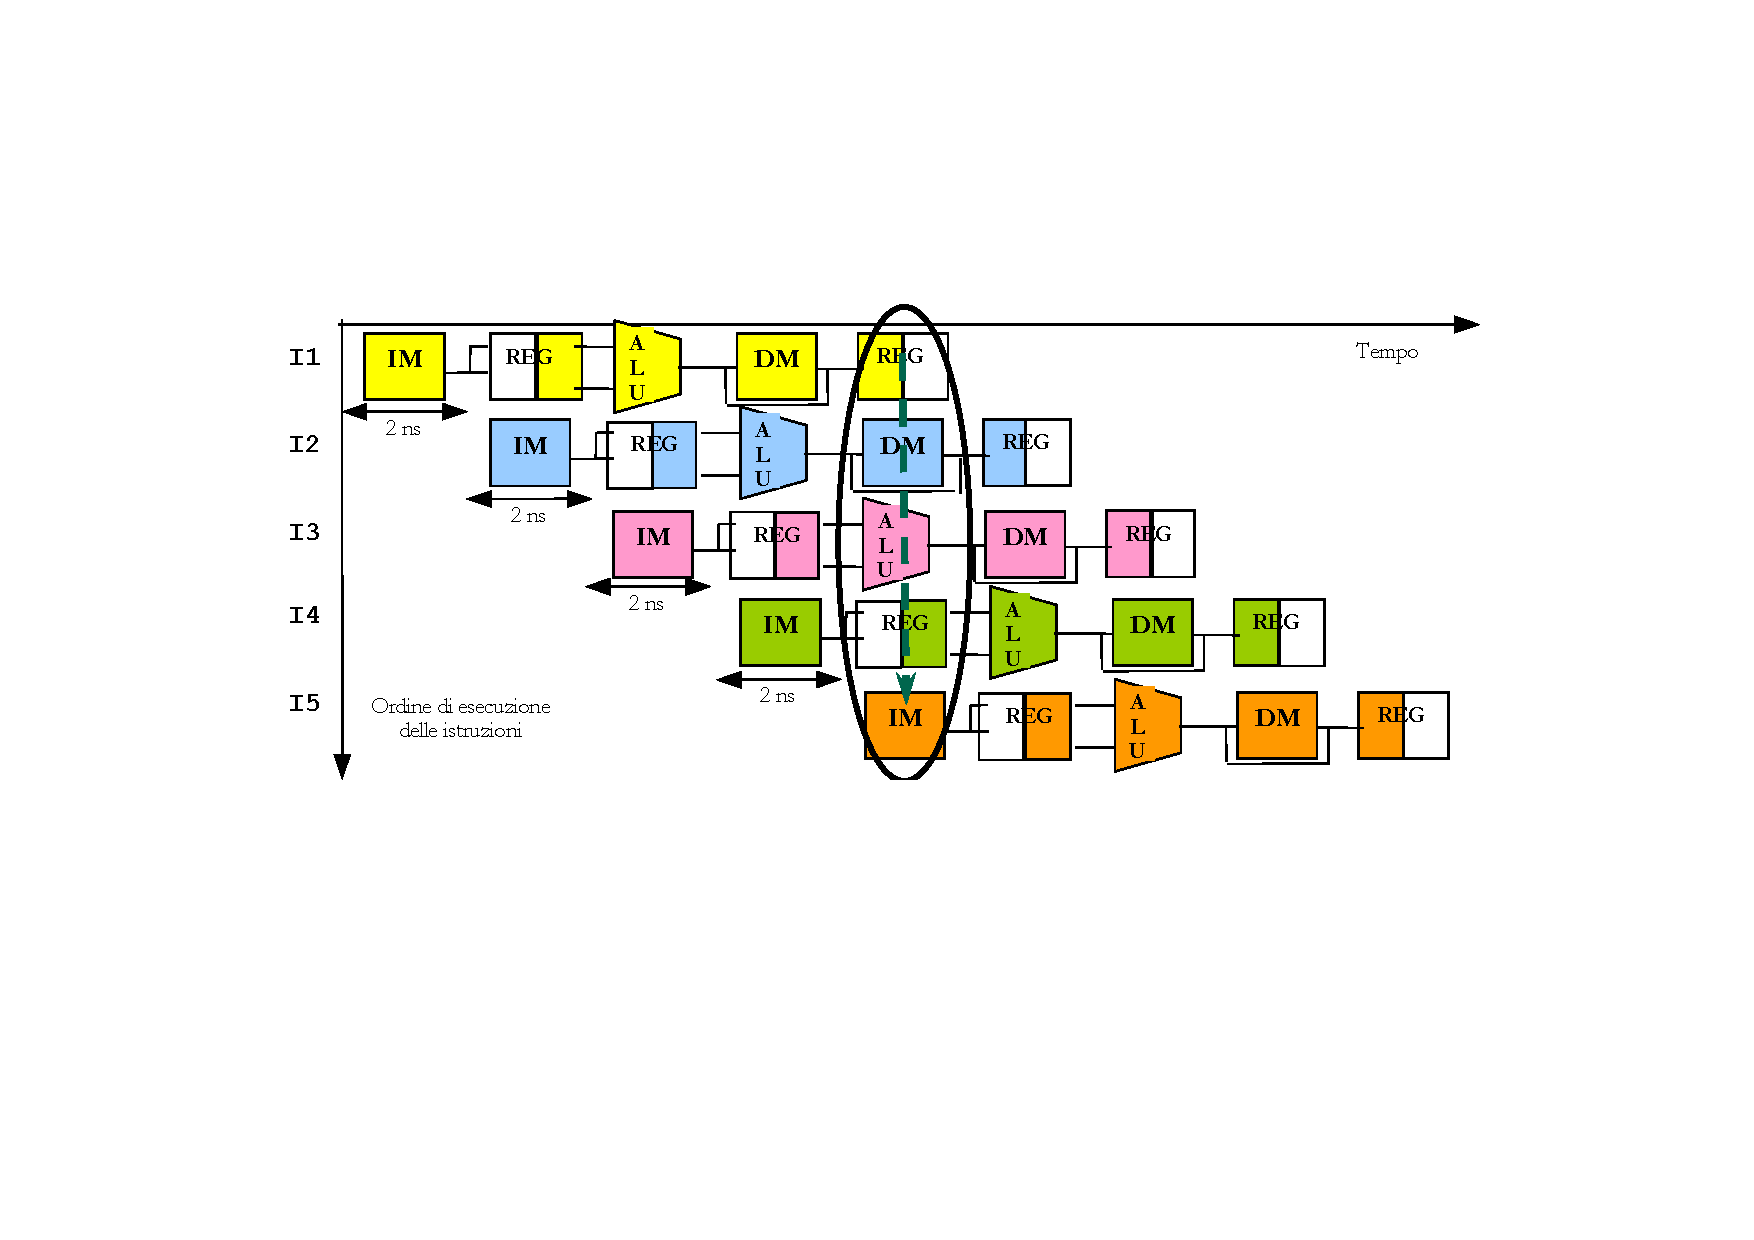
\includegraphics[width=\textwidth]{img/optimized-pipeline-1.pdf}
    \caption{Optimized Pipeline (IM is Instruction Memory, REG is Register File, and DM is Data Memory).\cite{pipelining-slides}}
    \label{fig: Optimized Pipeline}
\end{figure}

\noindent
And the problem mentioned at the beginning of this paragraph is partially solved, as we can see in the following figure.
\begin{figure}[!htp]
    \centering
    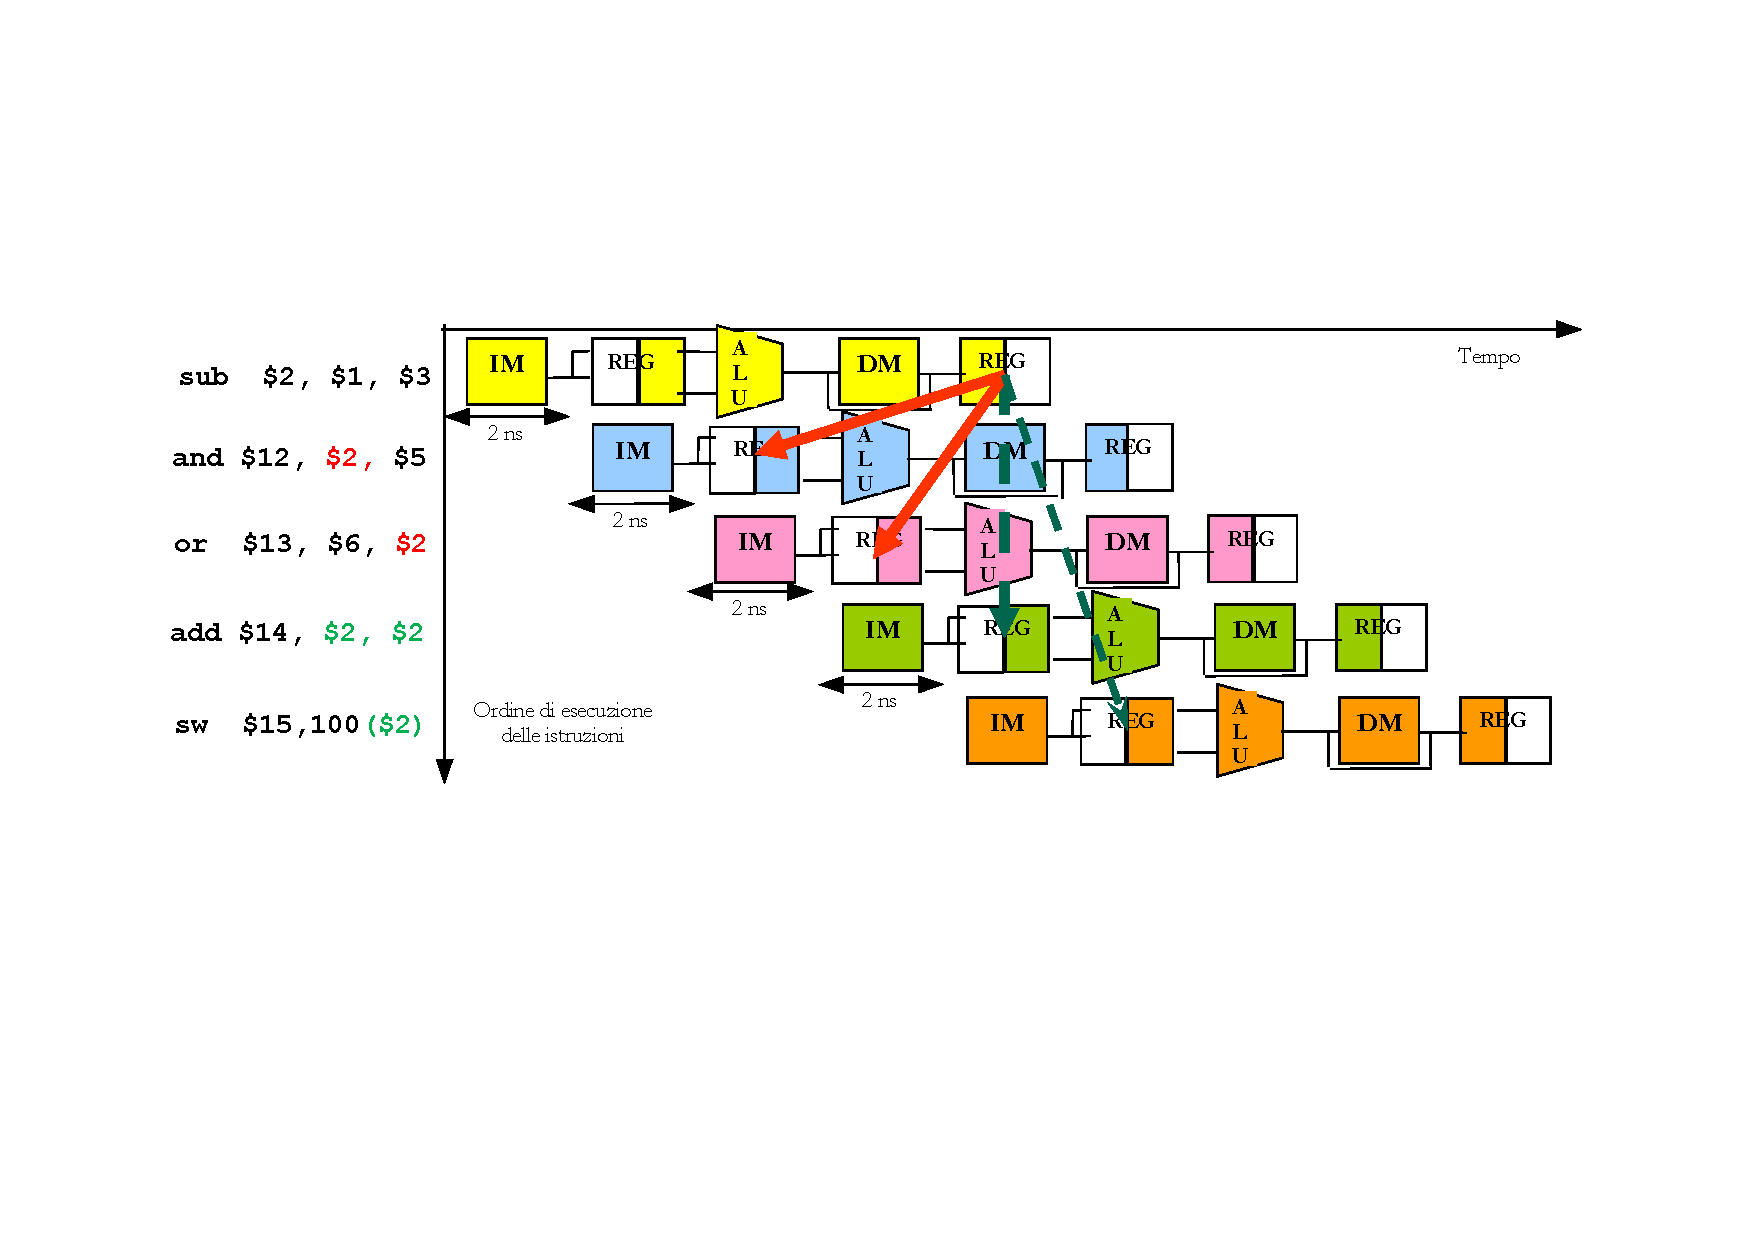
\includegraphics[width=\textwidth]{img/optimized-pipeline-2.pdf}
    \caption{Optimized Pipeline to solve the example stall.\cite{pipelining-slides}}
\end{figure}
    \subsubsection{The solution of Data Hazards}

The following techniques don't solve the problem completely, but they do solve it partially. So they find a perfect balance between the ideal speedup and a situation where the hazard is total.

\highspace
The solution can be applied on runtime (hardware techniques) or on compilation (static-time techniques):
\begin{itemize}
    \item \textbf{Compilation Techniques} (static-time techniques):
    \begin{itemize}
        \item The \definition{insertion of \texttt{nop}} is a simple (logical) solution where we \textbf{insert a \texttt{nop} operator between dependent statements} to ensure correct operation.

        See the \example{example} on page \pageref{example: insertion of nop}.


        \item The \definition{instructions scheduling} is a technique used by the compiler to prevent correlating instructions from being too close together. It tries to \textbf{reorder instructions} by inserting independent instructions between correlating instructions. \textbf{If the compiler can't do this, it inserts \texttt{nop} operations}.

        See the \example{example} on page \pageref{example: instructions scheduling}.
    \end{itemize}

    \item \textbf{Hardware Techniques} (runtime techniques):
    \begin{itemize}
        \item The \definition{insertion of stalls} (called also \emph{bubbling the pipeline}, \emph{pipeline break}, or \emph{pipeline stall}) is a sort of a delay before the processor can resume execution of the instruction. As we can see in the \example{example} on page \pageref{example: insertion of stalls}, the stalls delay the stages of the correlating instructions.

        \item The \definition{data forwarding} \textbf{uses temporary results stored in the pipeline registers} instead of waiting for the results to be written back to the Register File (RF). To do this, it's \textbf{necessary to add new paths and multiplexers at the inputs of the ALU} to fetch inputs from the pipeline to avoid inserting stalls in the pipeline.

        See the \example{example} on page \pageref{example: data forwarding}.
    \end{itemize}
\end{itemize}
We have the mandatory to give more words to the data forwarding technique. First of all, its implementation needs new paths and new multiplexers. So, to adapt the MIPS architecture, the new implementation will be show in the figure \ref{fig: implementation of MIPS with Forwarding Unit} on page \pageref{fig: implementation of MIPS with Forwarding Unit}.

\newpage

\begin{figure}[!htp]
    \centering
    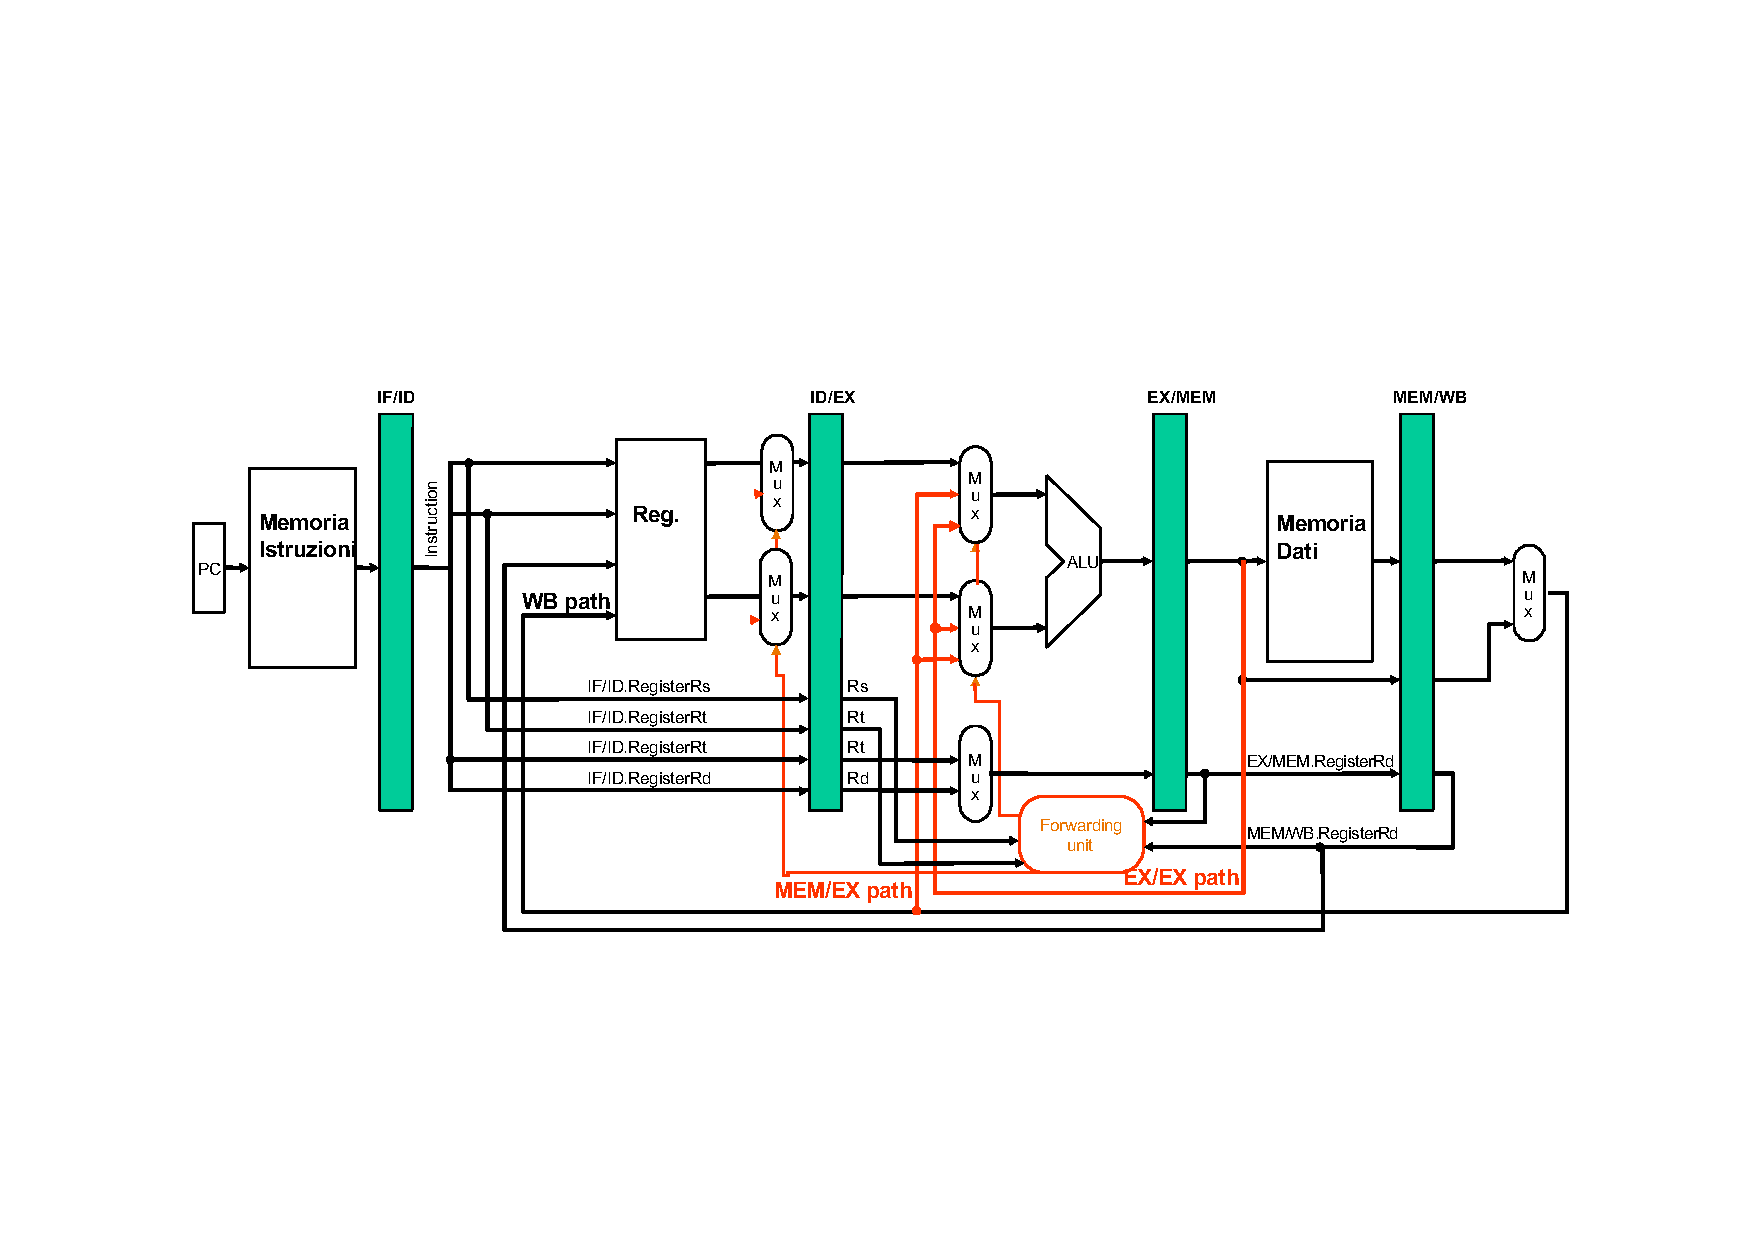
\includegraphics[width=\textwidth]{img/implementation-mips-forwarding-unit-1.pdf}
    \caption{Implementation of MIPS with \definition{Forwarding Unit}.\cite{pipelining-slides}}
    \label{fig: implementation of MIPS with Forwarding Unit}
\end{figure}

\noindent
Scan (or click) the QR code below to view the figure~\ref{fig: implementation of MIPS with Forwarding Unit} in high quality:
\begin{center}
    \qrcode{https://github.com/PoliMI-HPC-E-notes-projects-AndreVale69/HPC-E-PoliMI-university-notes/tree/main/advanced-computer-architectures/notes/img/implementation-mips-forwarding-unit-1.pdf}
\end{center}

\noindent
The forwarding paths created inside the MIPS architecture are three: \textbf{\texttt{EX} to \texttt{EX}} path, \textbf{\texttt{MEM} to \texttt{EX}} path, and \textbf{\texttt{MEM} to \texttt{MEM}} path.
\begin{figure}[!htp]
    \centering
    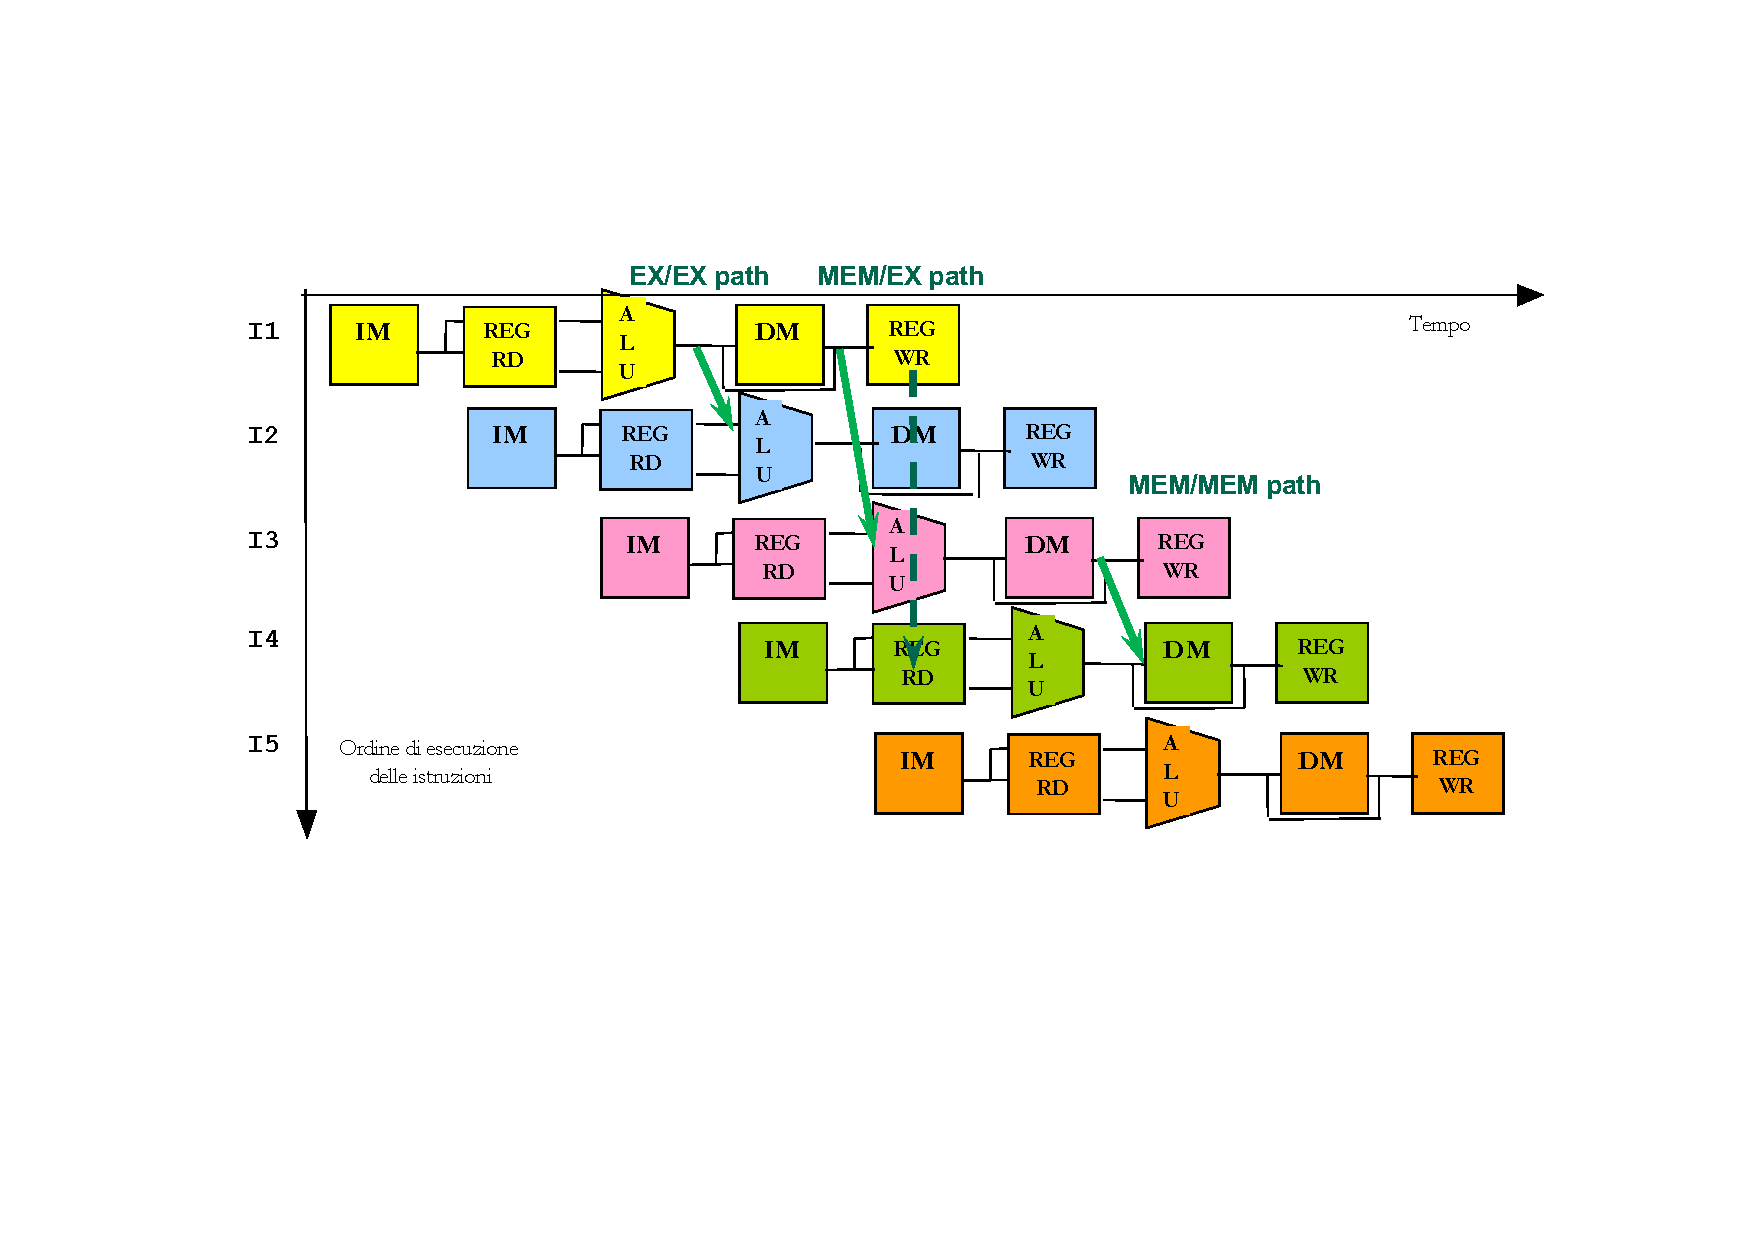
\includegraphics[width=\textwidth]{img/forwarding-paths-1.pdf}
    \caption{Forwarding paths on MIPS architecture.\cite{pipelining-slides}}
\end{figure}

\noindent
Furthermore, the \textbf{forwarding technique can solve} the \textbf{Load-Use} and \textbf{Load-Store} Data Hazard. It's a very interesting feature because the \texttt{MEM} to \texttt{EX} and \texttt{MEM} to \texttt{MEM} paths can solve two different situations:
\begin{itemize}
    \item \textbf{Load-Use} Hazard. It's \textbf{solved by MEM to EX path} because the value loaded in the MEM stage, is forwarded directly to the EX stage of the next conflict instruction (but unfortunately we need one stall to delay the run).

    \begin{examplebox}
        Given the following code:
        \lstinputlisting[language=misc]{code/solution-of-data-hazards/load-use-hazard-1.s}
        The \texttt{s0} operand depends on the load (\texttt{lw}) operator. Here, the problem of \textbf{\emph{load-use hazard}} occurs.
        \begin{center}
            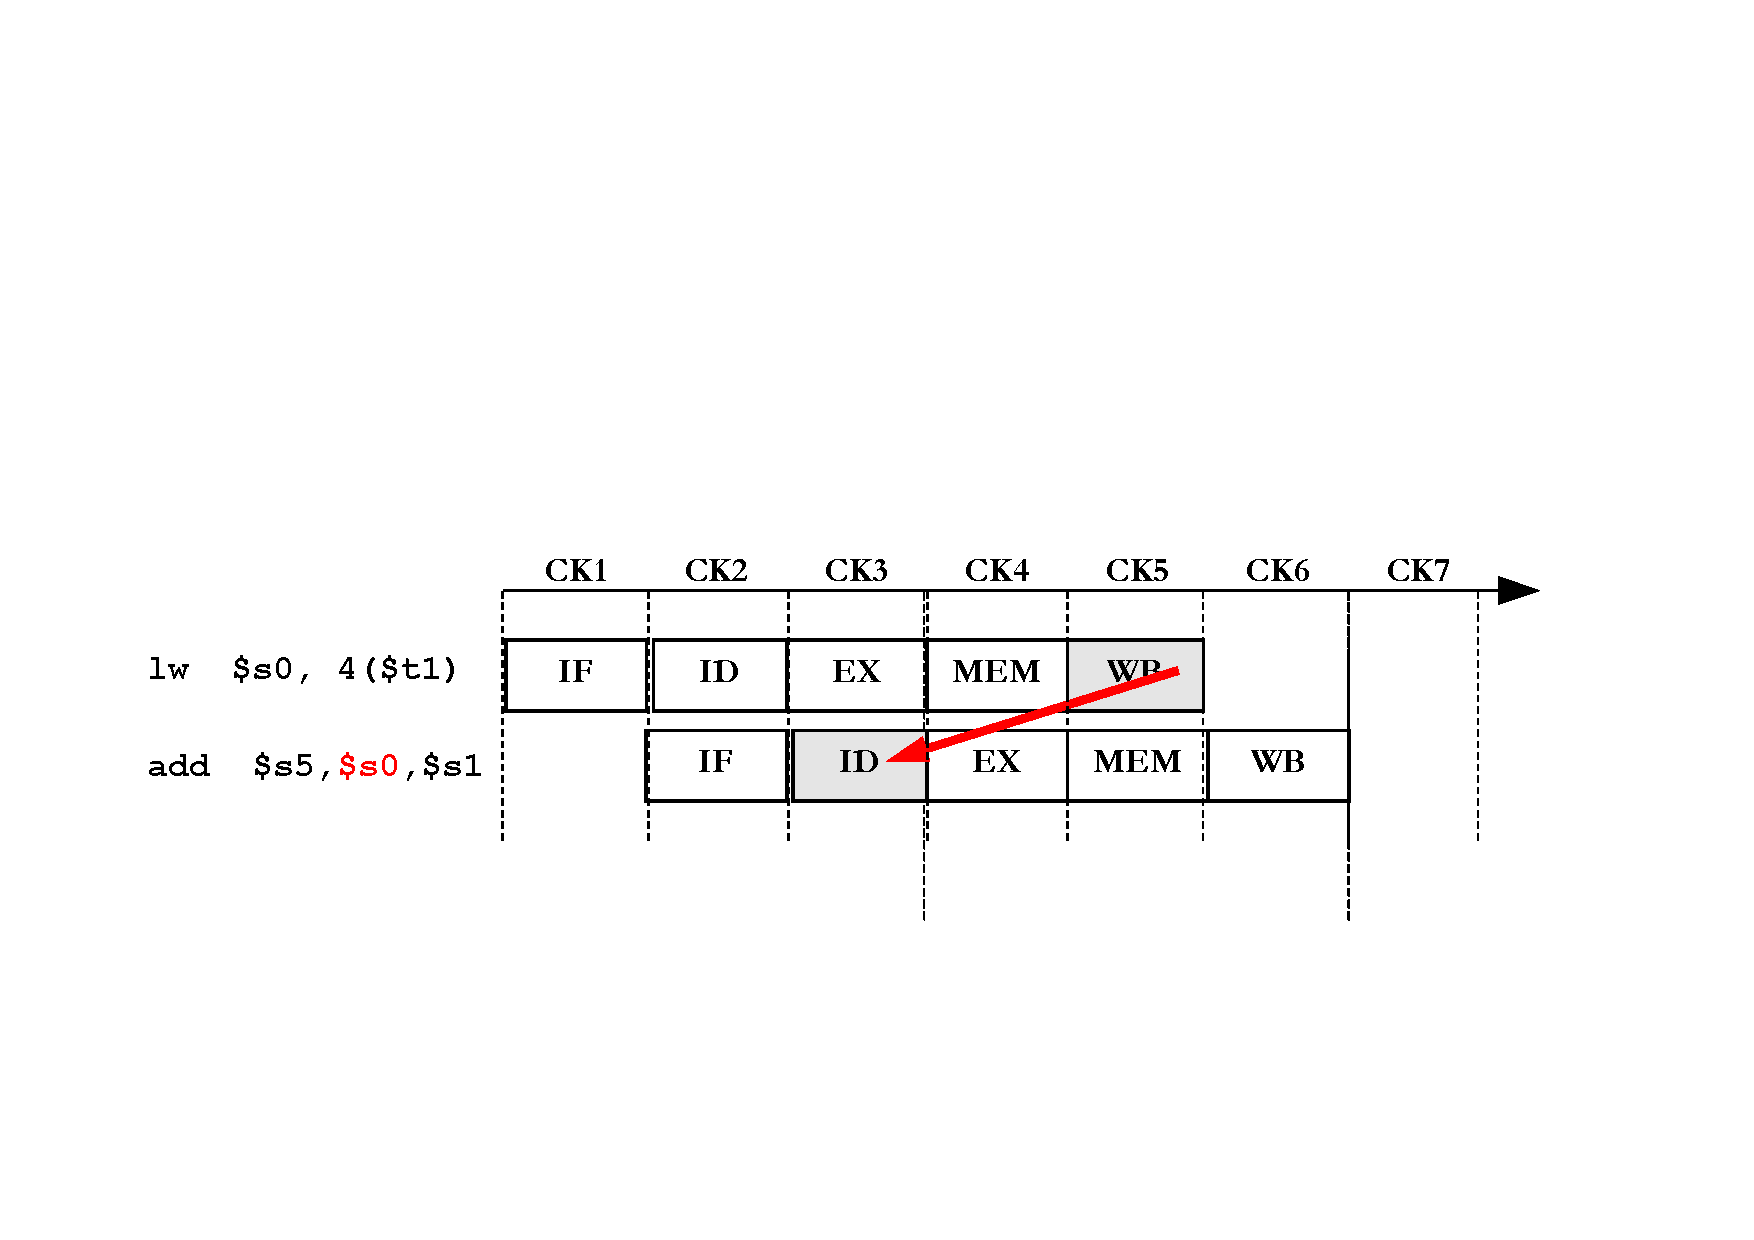
\includegraphics[width=\textwidth]{img/load-use-hazard-problem-1.pdf}
            \captionof*{figure}{The load-use hazard problem.\cite{pipelining-slides}}
        \end{center}
        In the figure, we can see the existing dependence. An ideal solution to the load-use hazard should be taking the value after the Memory Access operation (because the load instruction reads the effective address on the memory) and using it in the sum (operation).

        The \textbf{forwarding technique solves it using the MEM-EX path but using \underline{one stall}}.
        \begin{center}
            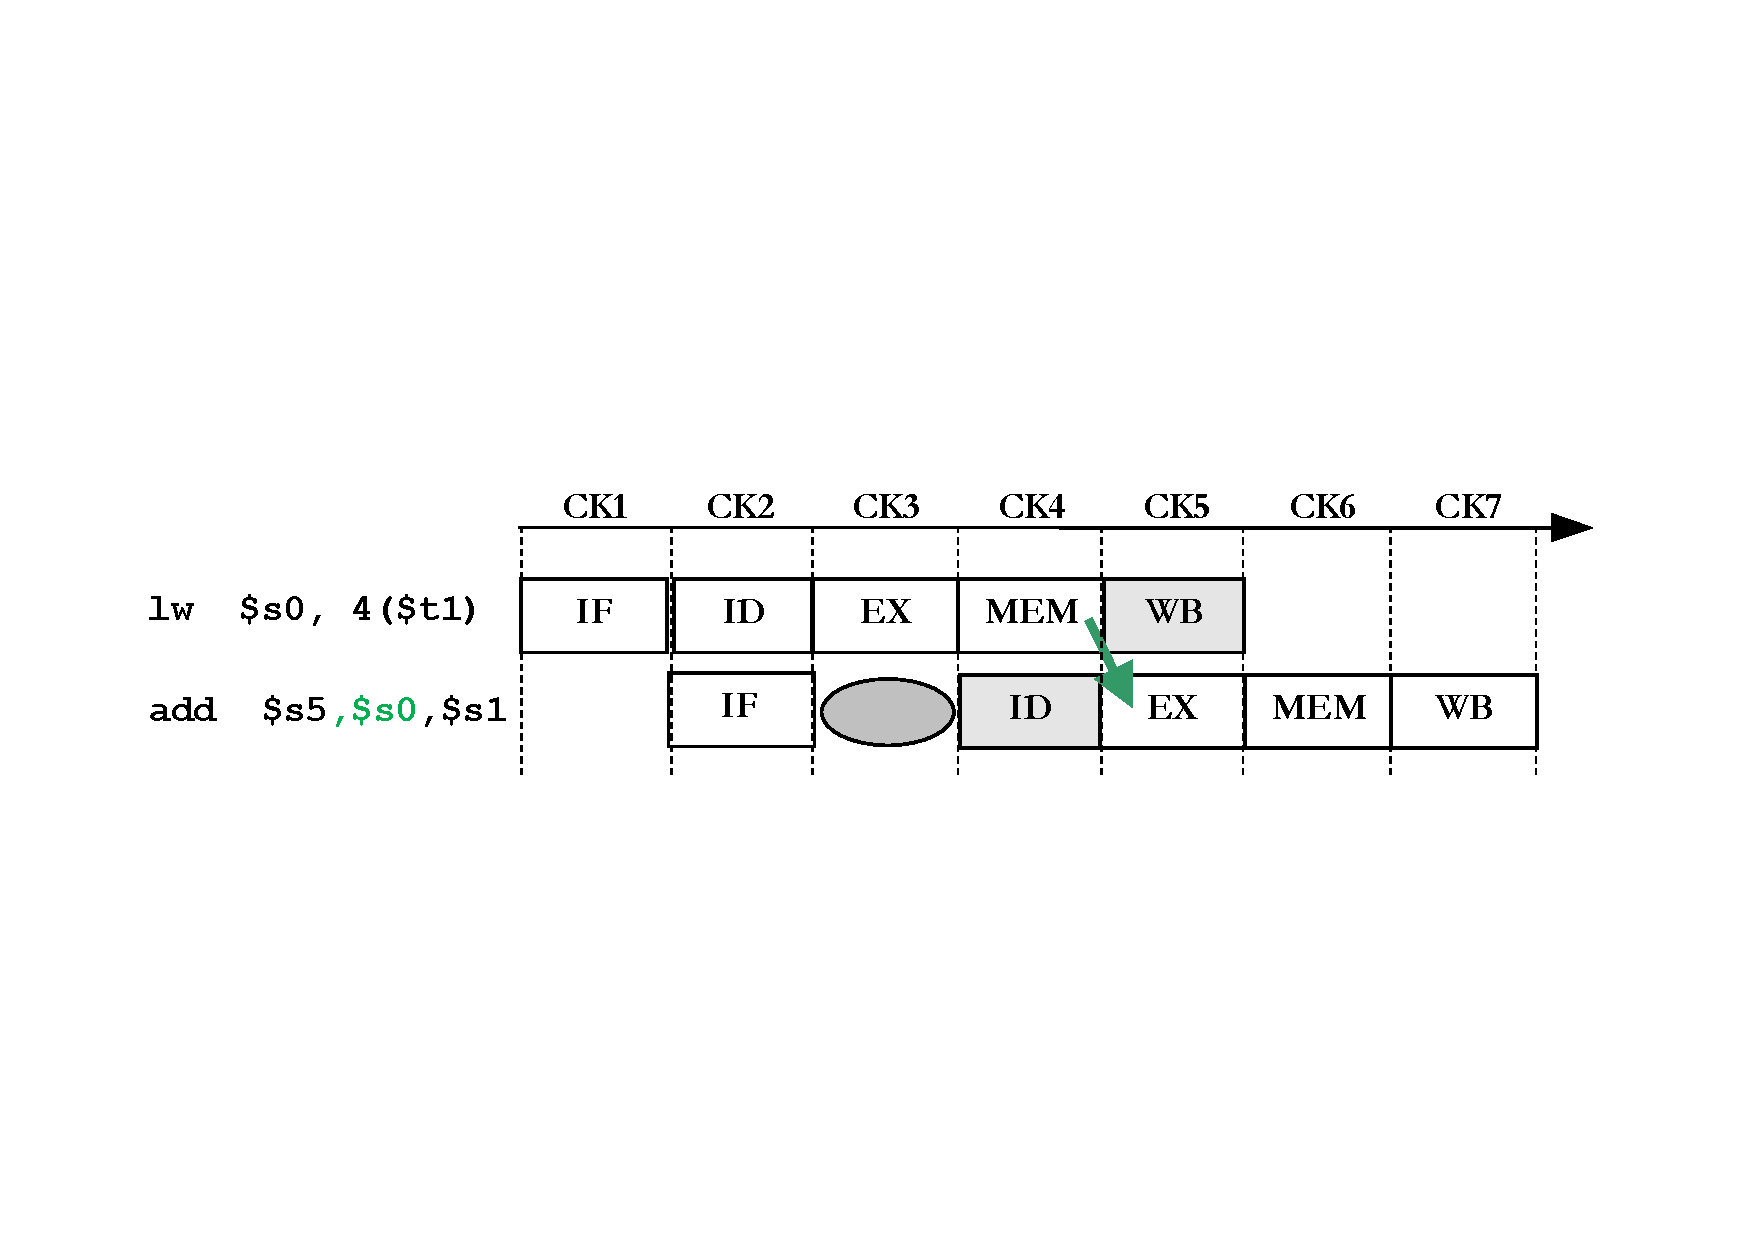
\includegraphics[width=\textwidth]{img/load-use-hazard-problem-2.pdf}
            \captionof*{figure}{Forwarding technique with MEM-EX path.\cite{pipelining-slides}}
        \end{center}
    \end{examplebox}
    % TODO: add example

    \item \textbf{Load-Store} Hazard. It's \textbf{solved by MEM to MEM path} because the value loaded in the MEM stage, is forwarded directly to the MEM stage of the next conflict instruction.
    \begin{examplebox}
        Given the following code:
        \lstinputlisting[language=misc]{code/solution-of-data-hazards/load-store-hazard-1.s}
        The \texttt{s0} operand depends on the load (\texttt{lw}) operator. Here, the problem of \textbf{\emph{load-store hazard}} occurs.
        \begin{center}
            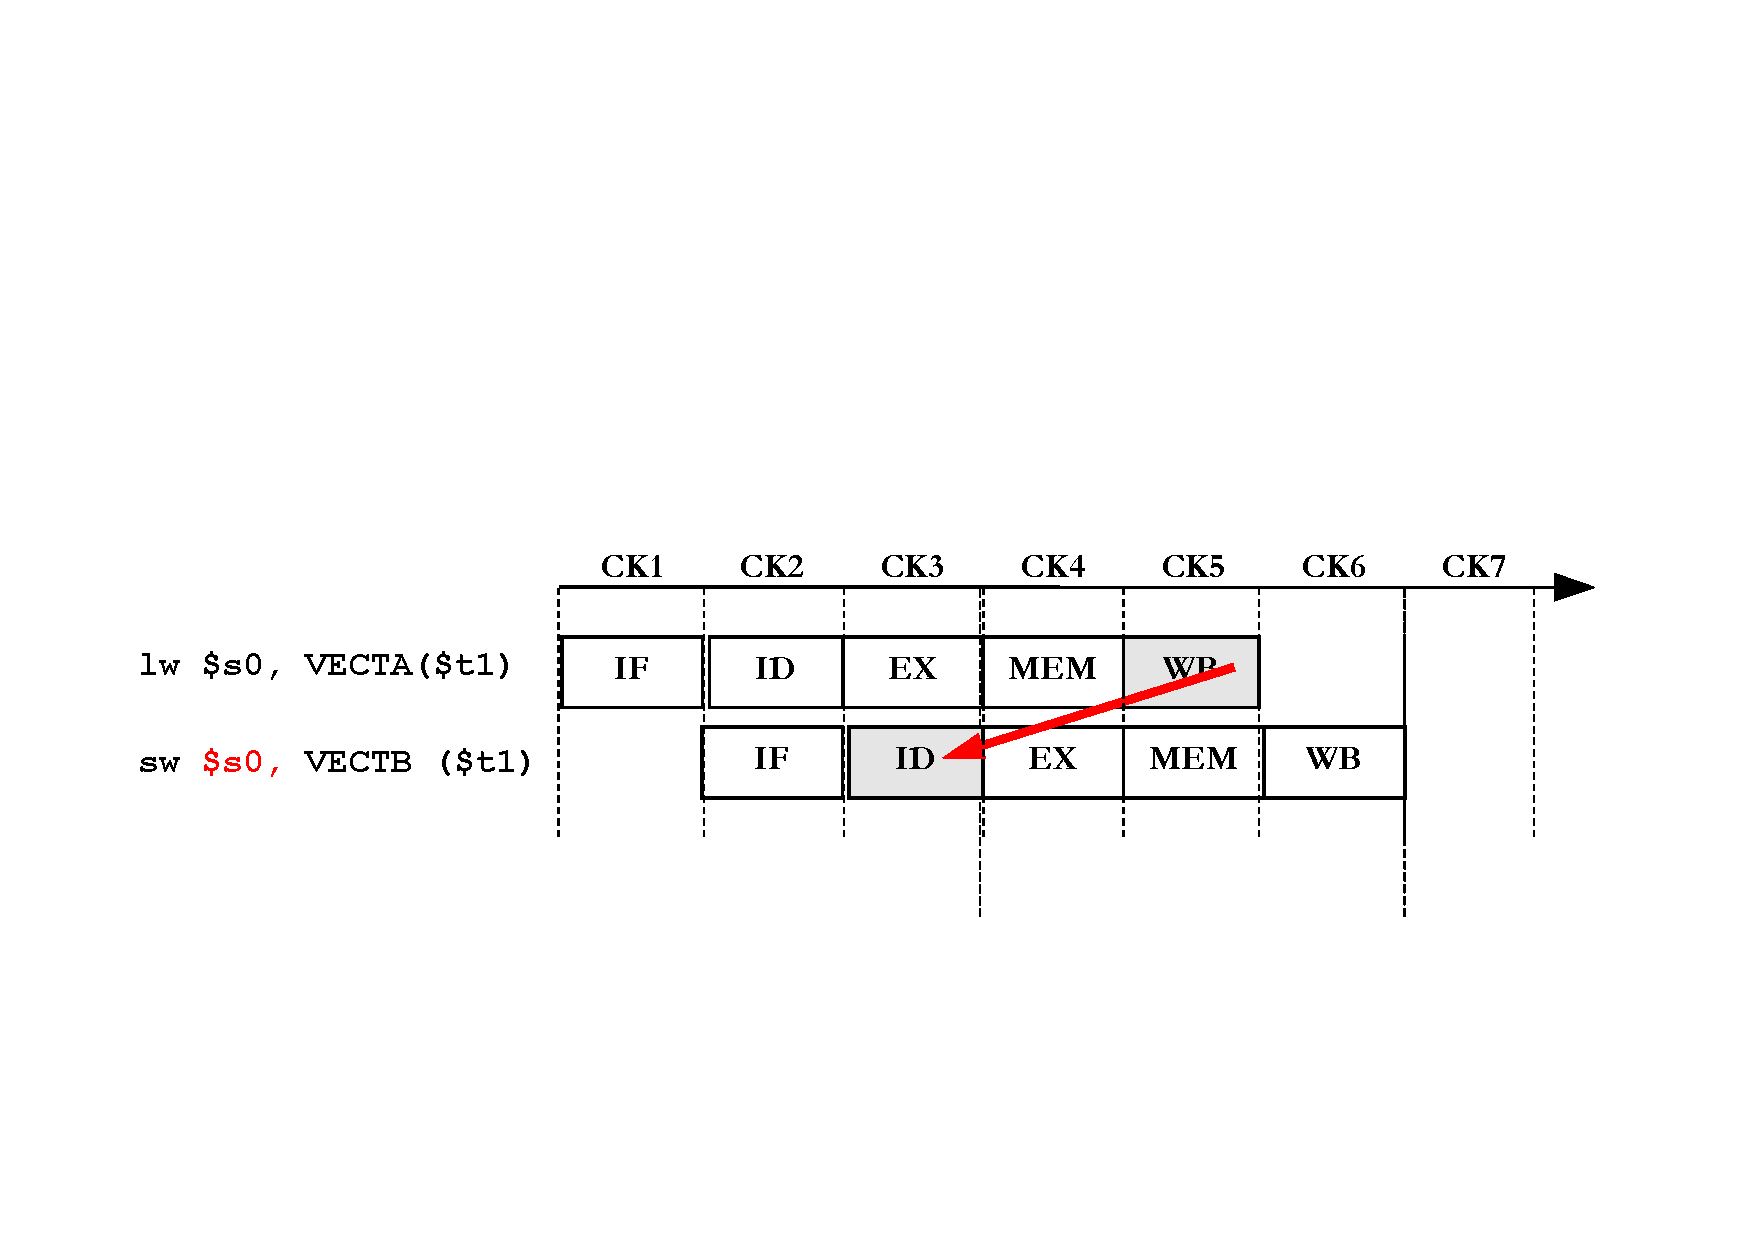
\includegraphics[width=\textwidth]{img/load-store-hazard-problem-1.pdf}
            \captionof*{figure}{The load-store hazard problem.\cite{pipelining-slides}}
        \end{center}
        In the figure, we can see the existing dependence. An ideal solution to the load-store hazard should be taking the value after the Write Back operation (because the load instruction writes the data read from memory in the destination register of the Register File) and using it in the Instruction Decode (because the ID includes also Register Read, then it reads from the Register File (RF)).

        The \textbf{forwarding technique solves it using the MEM-MEM path \underline{without any stall}}.
        \begin{center}
            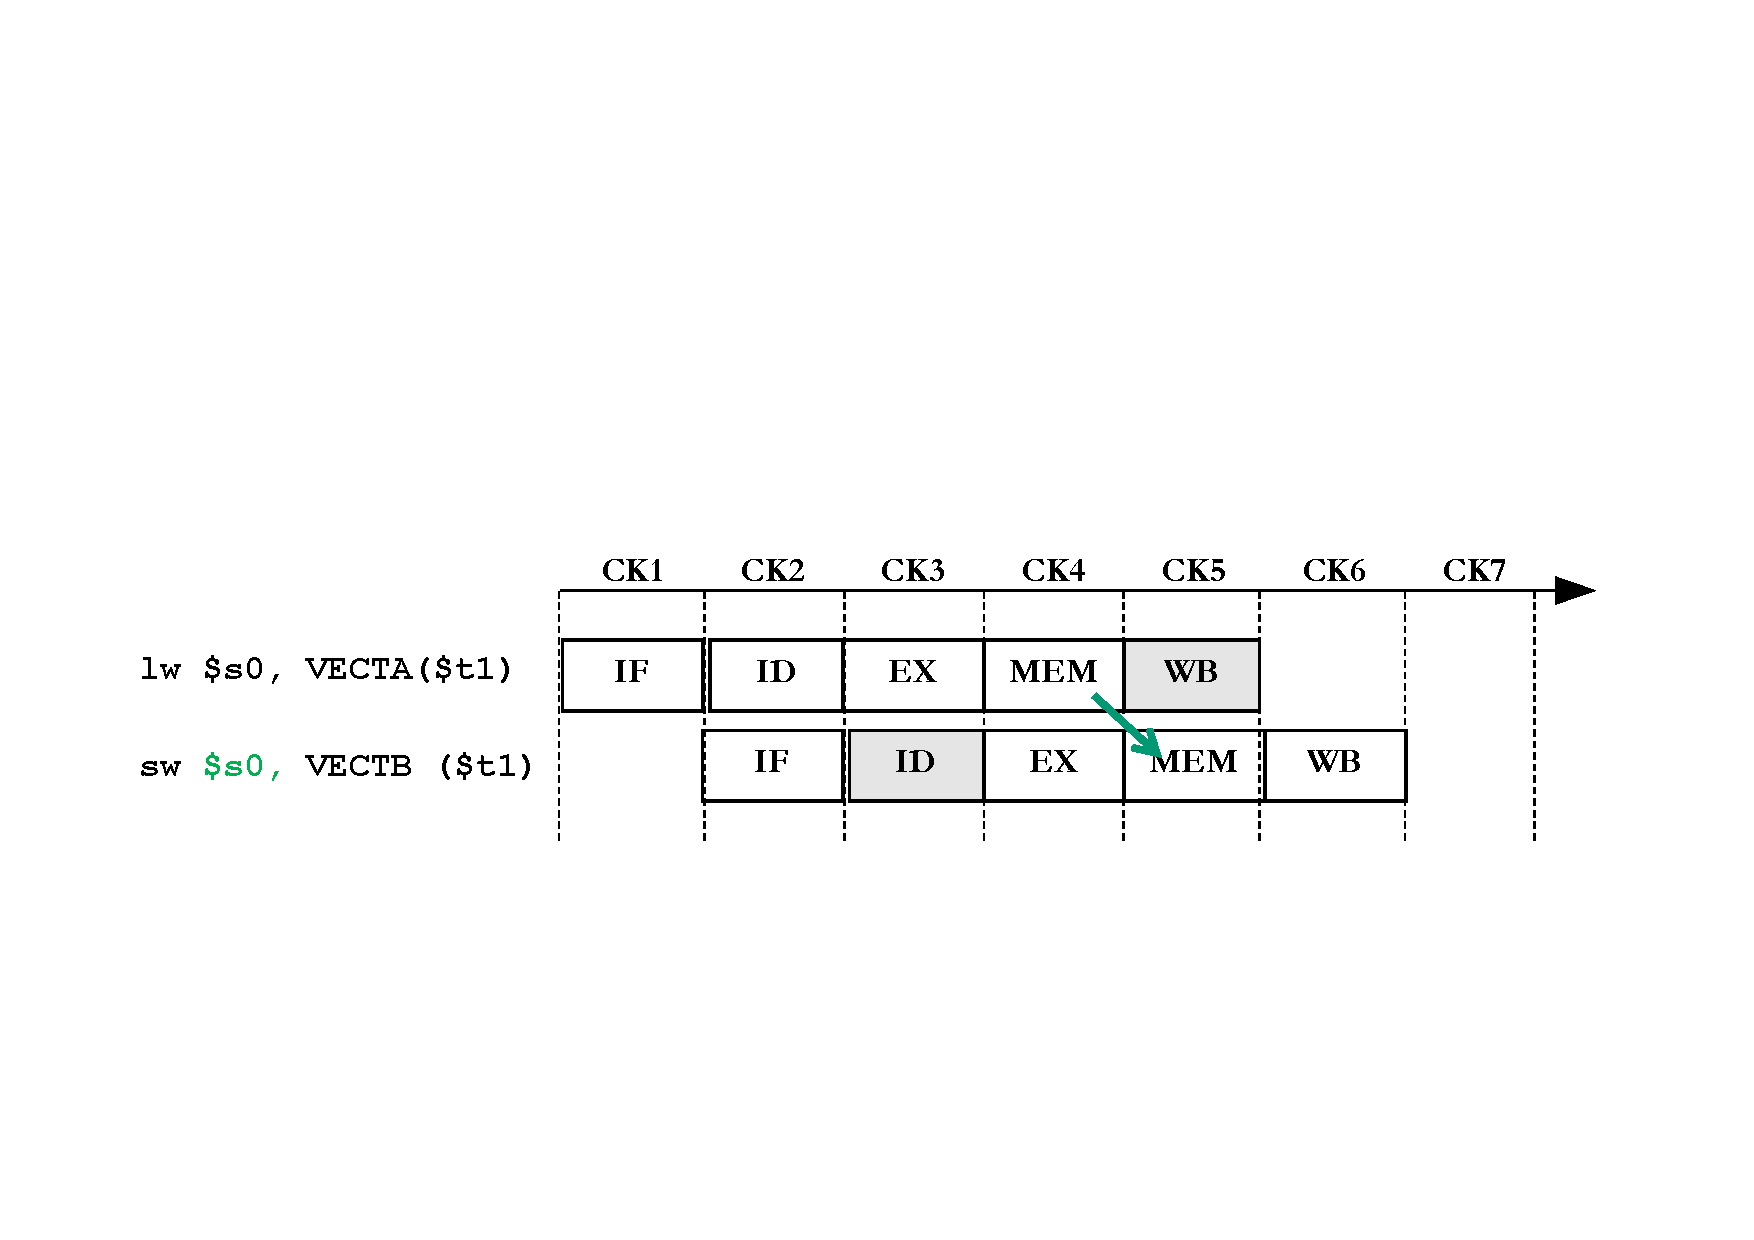
\includegraphics[width=\textwidth]{img/load-store-hazard-problem-2.pdf}
            \captionof*{figure}{Forwarding technique with MEM-MEM path.\cite{pipelining-slides}}
        \end{center}
    \end{examplebox}
\end{itemize}

\begin{examplebox}\label{example: insertion of nop}
    In the following figure, we can see how a \textbf{compilation technique}, the \textbf{insertion of \texttt{nop}}, can be solve the data hazard problem.
    \begin{center}
        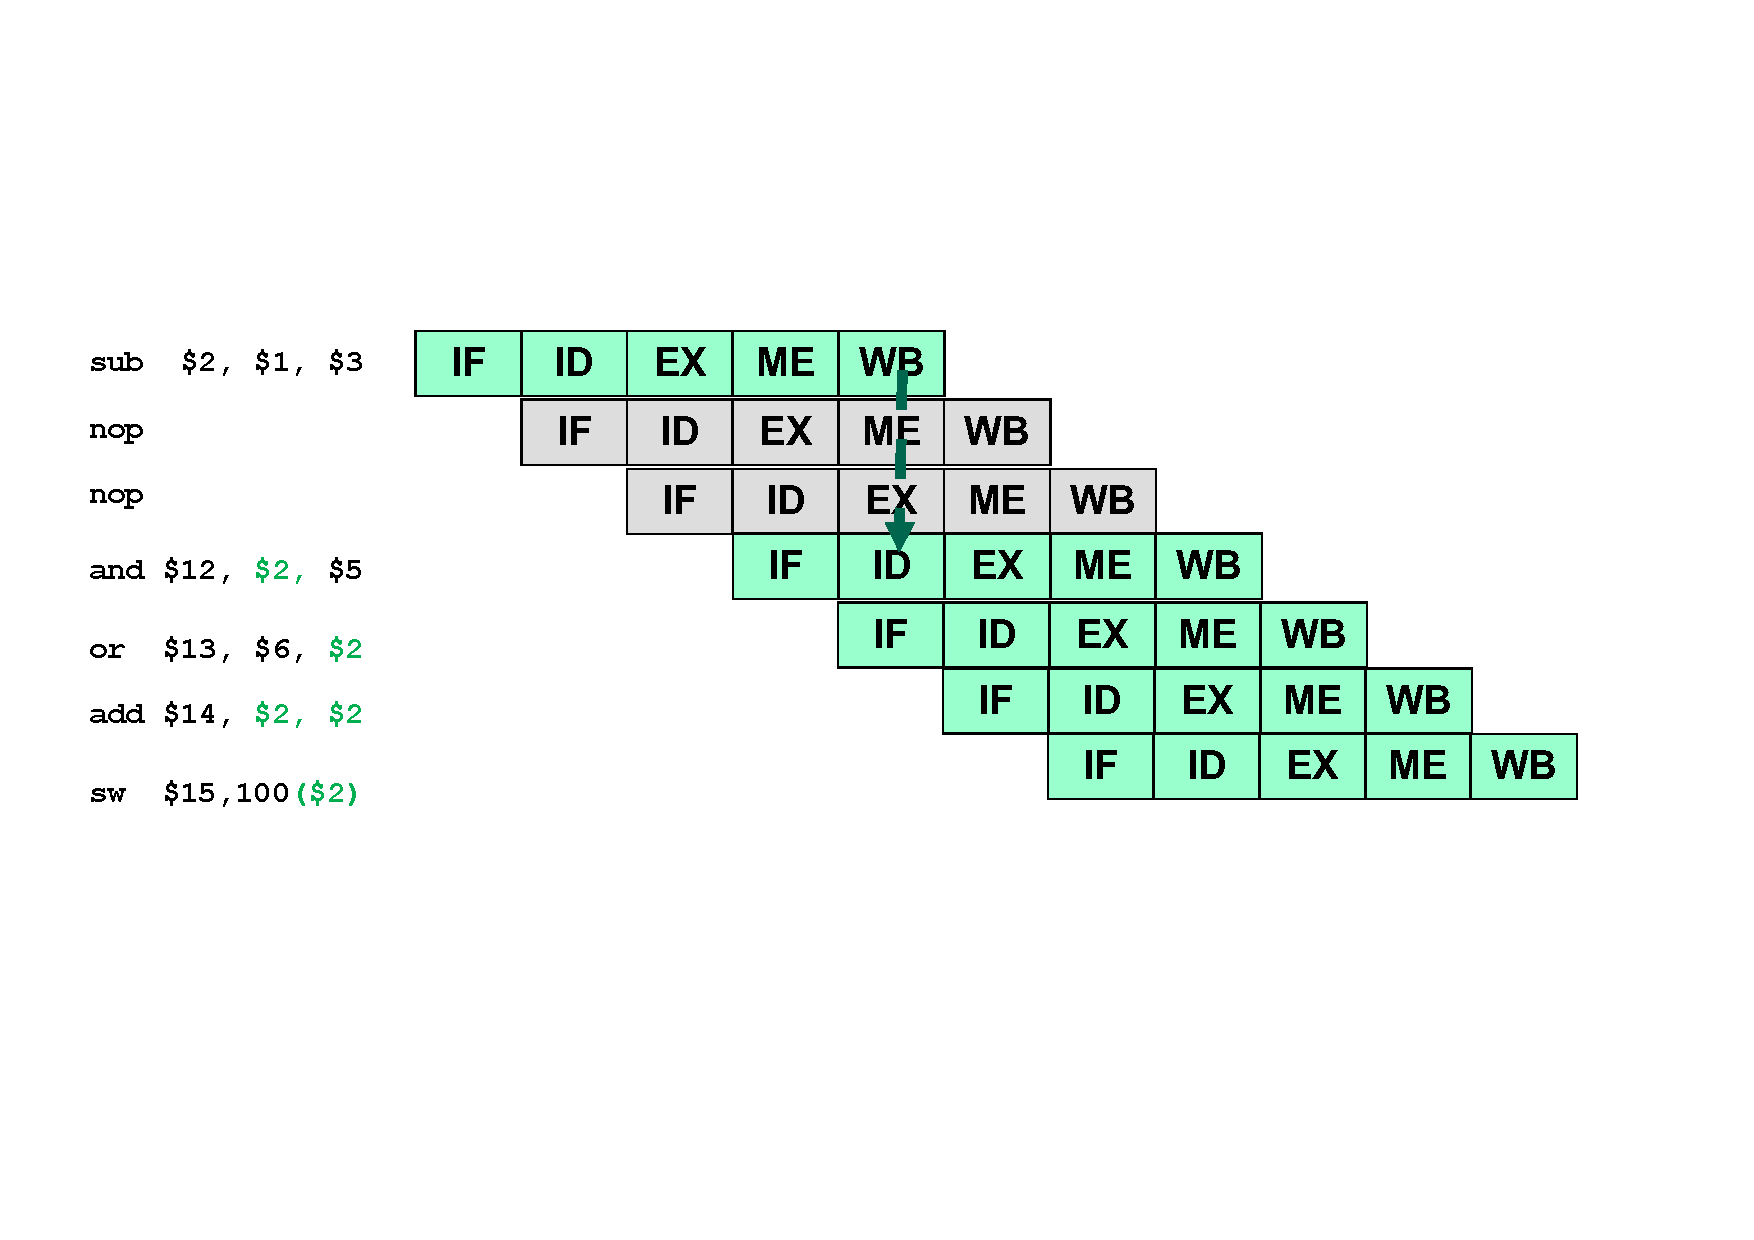
\includegraphics[width=\textwidth]{img/insertion-of-nop-1.pdf}
        \captionof*{figure}{Insertion of \texttt{nop}.\cite{pipelining-slides}}
    \end{center}
\end{examplebox}

\newpage

\begin{examplebox}\label{example: instructions scheduling}
    In the following figure, we can see how a \textbf{compilation technique}, the \textbf{instructions scheduling}, can be solve the data hazard problem.
    \begin{center}
        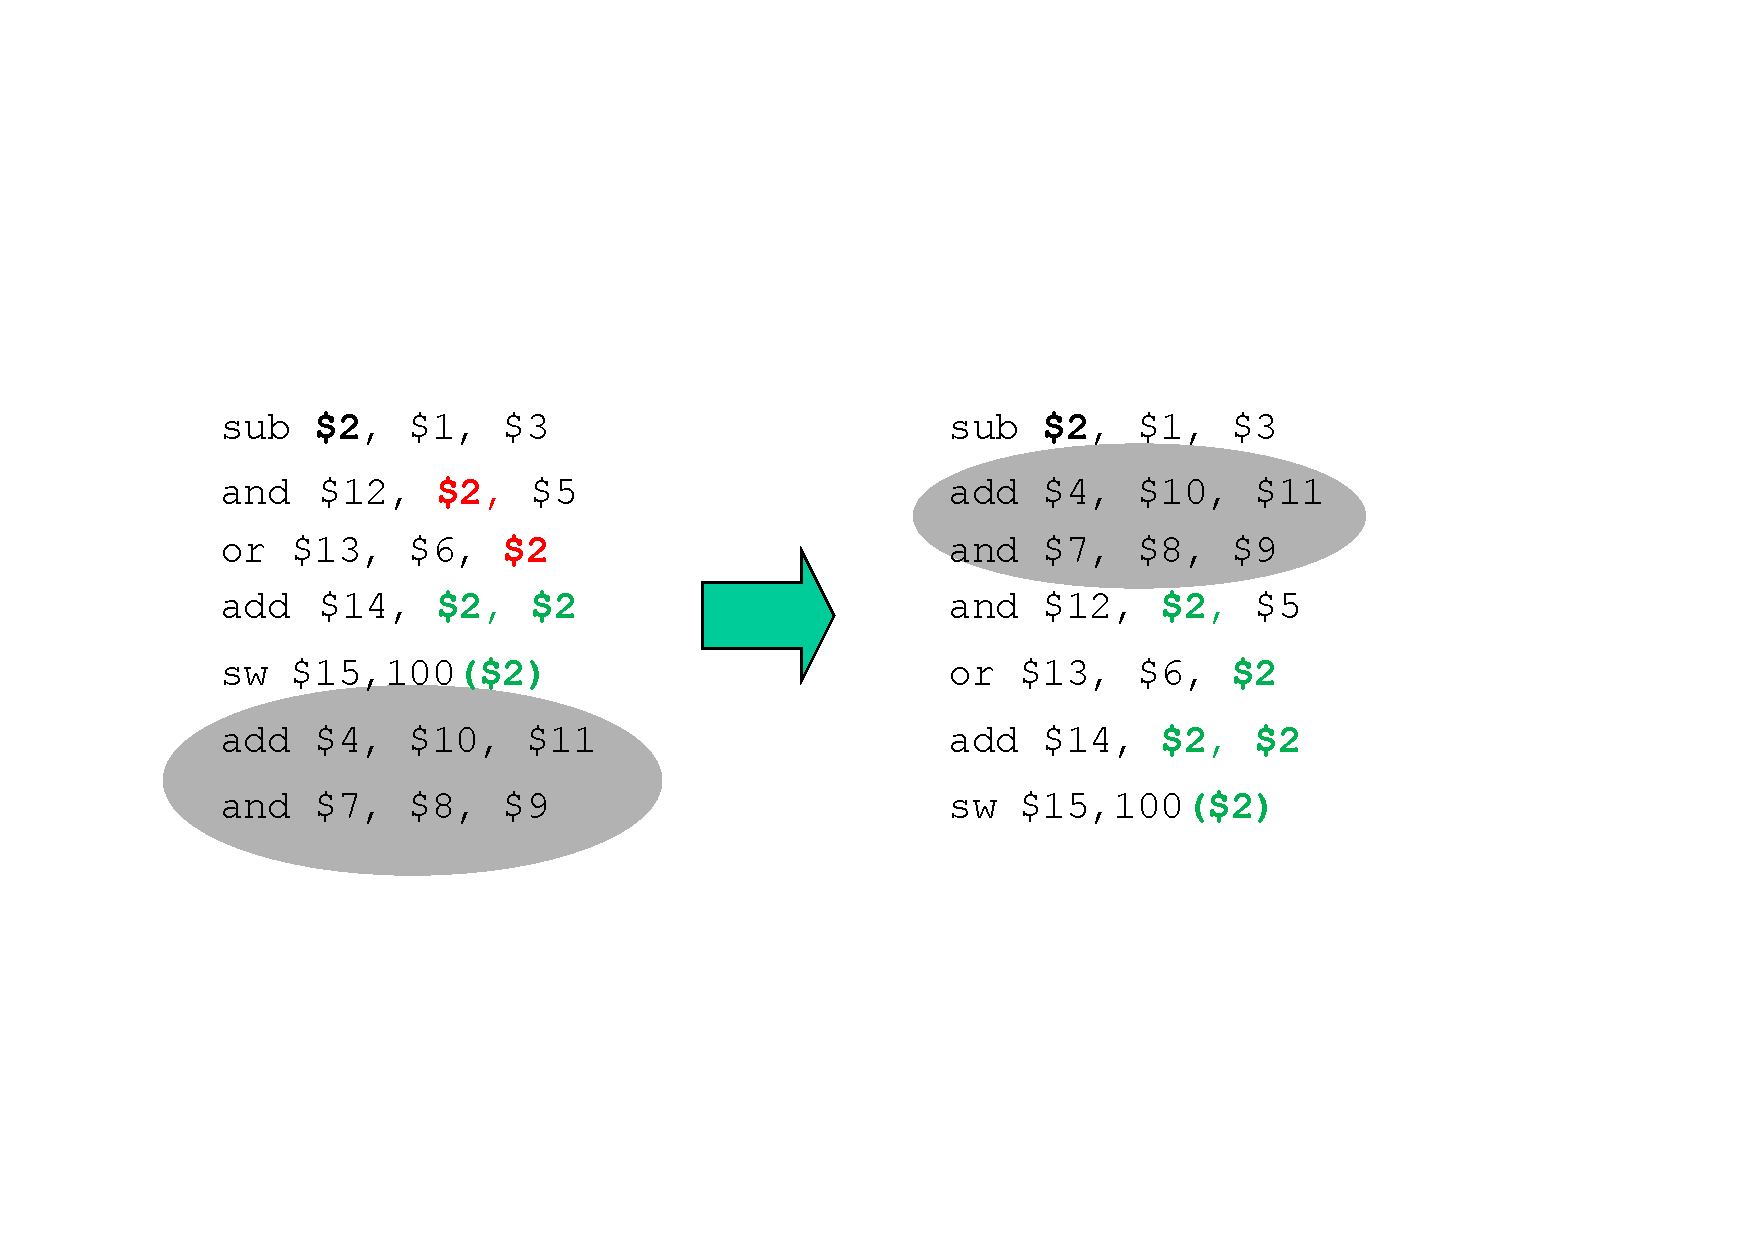
\includegraphics[width=\textwidth]{img/instructions-scheduling-1.pdf}
        \captionof*{figure}{Instructions scheduling.\cite{pipelining-slides}}
    \end{center}
\end{examplebox}

\begin{examplebox}\label{example: insertion of stalls}
    In the following figure, we can see how a \textbf{hardware technique}, the \textbf{insertion of stalls}, can be solve the data hazard problem.
    \begin{center}
        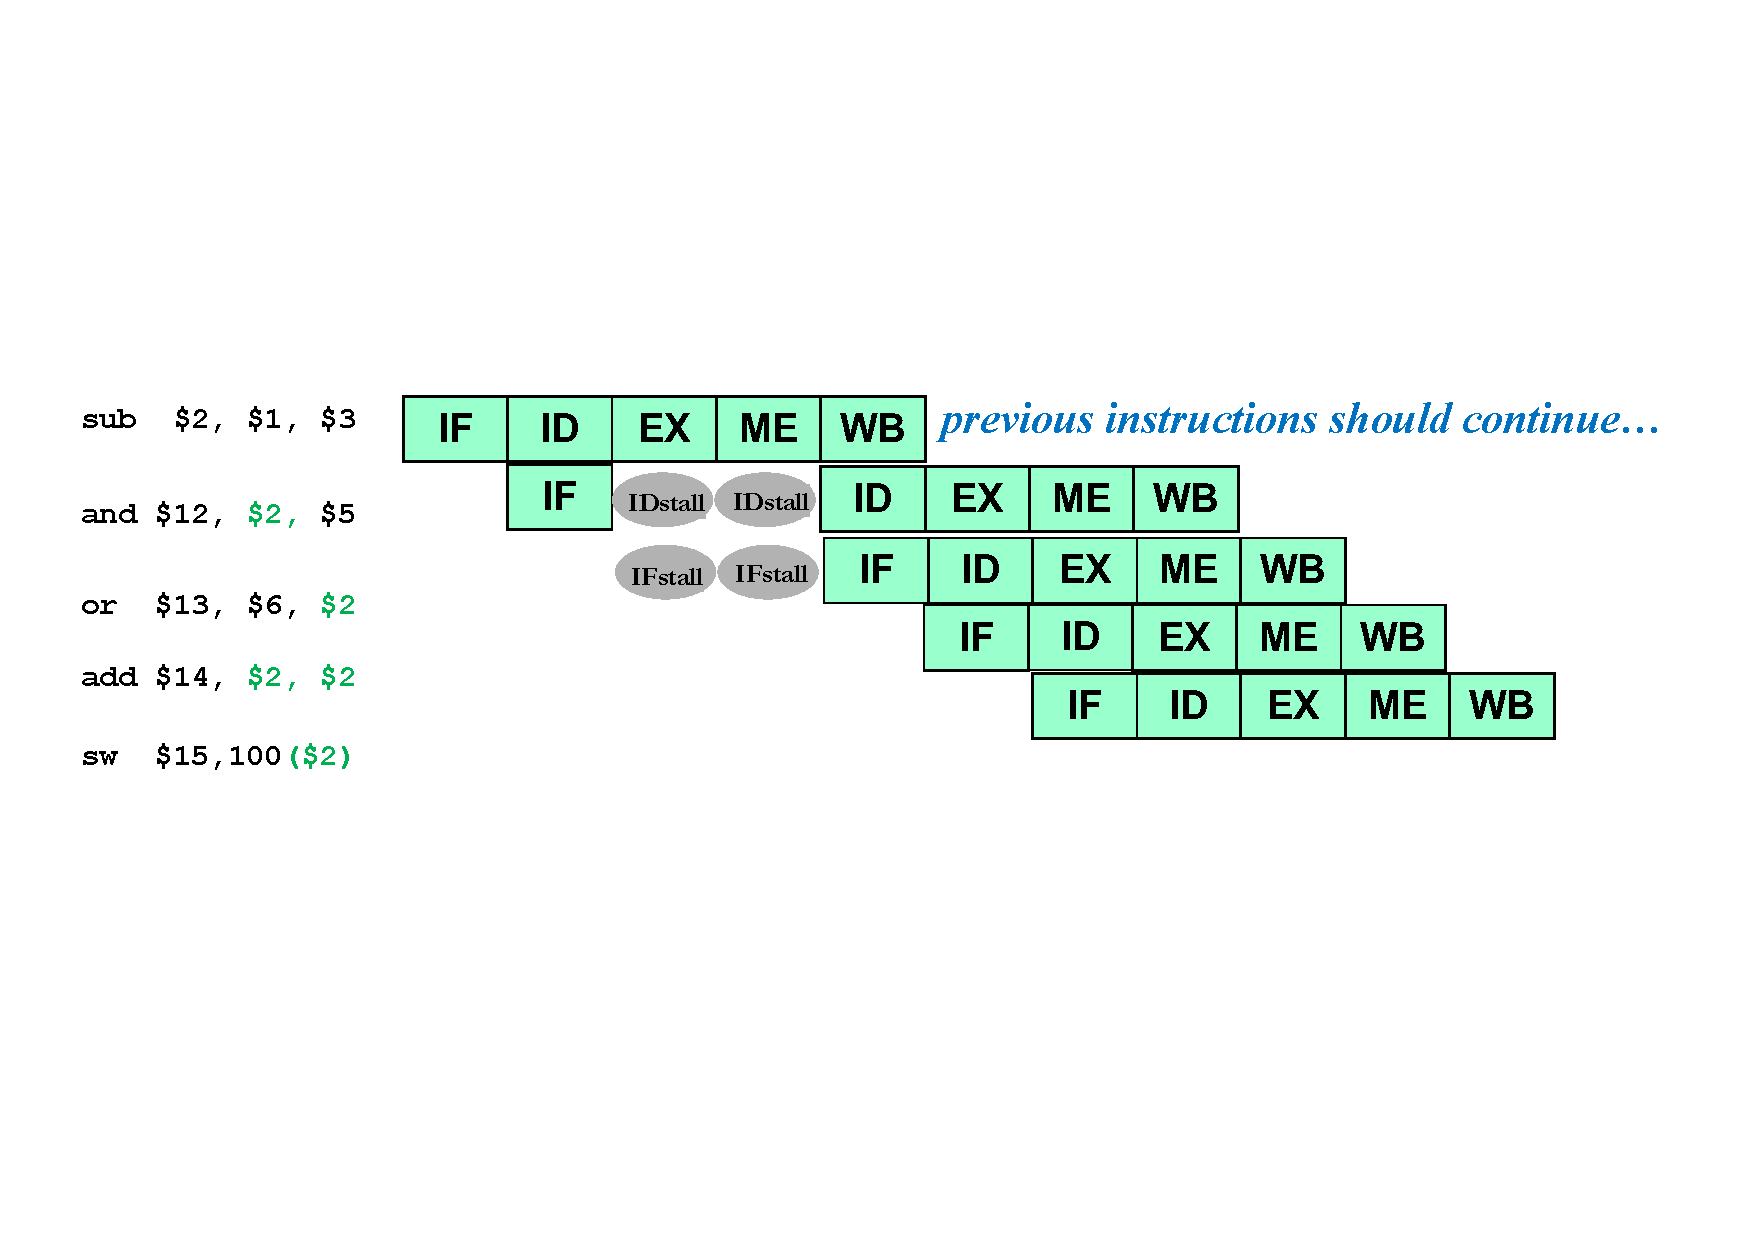
\includegraphics[width=\textwidth]{img/insertion-of-stalls-1.pdf}
        \captionof*{figure}{Insertion of stalls.\cite{pipelining-slides}}
    \end{center}
\end{examplebox}

\begin{examplebox}\label{example: data forwarding}
    In the following figure, we can see how a \textbf{hardware technique}, the \textbf{data forwarding}, can be solve the data hazard problem.
    \begin{center}
        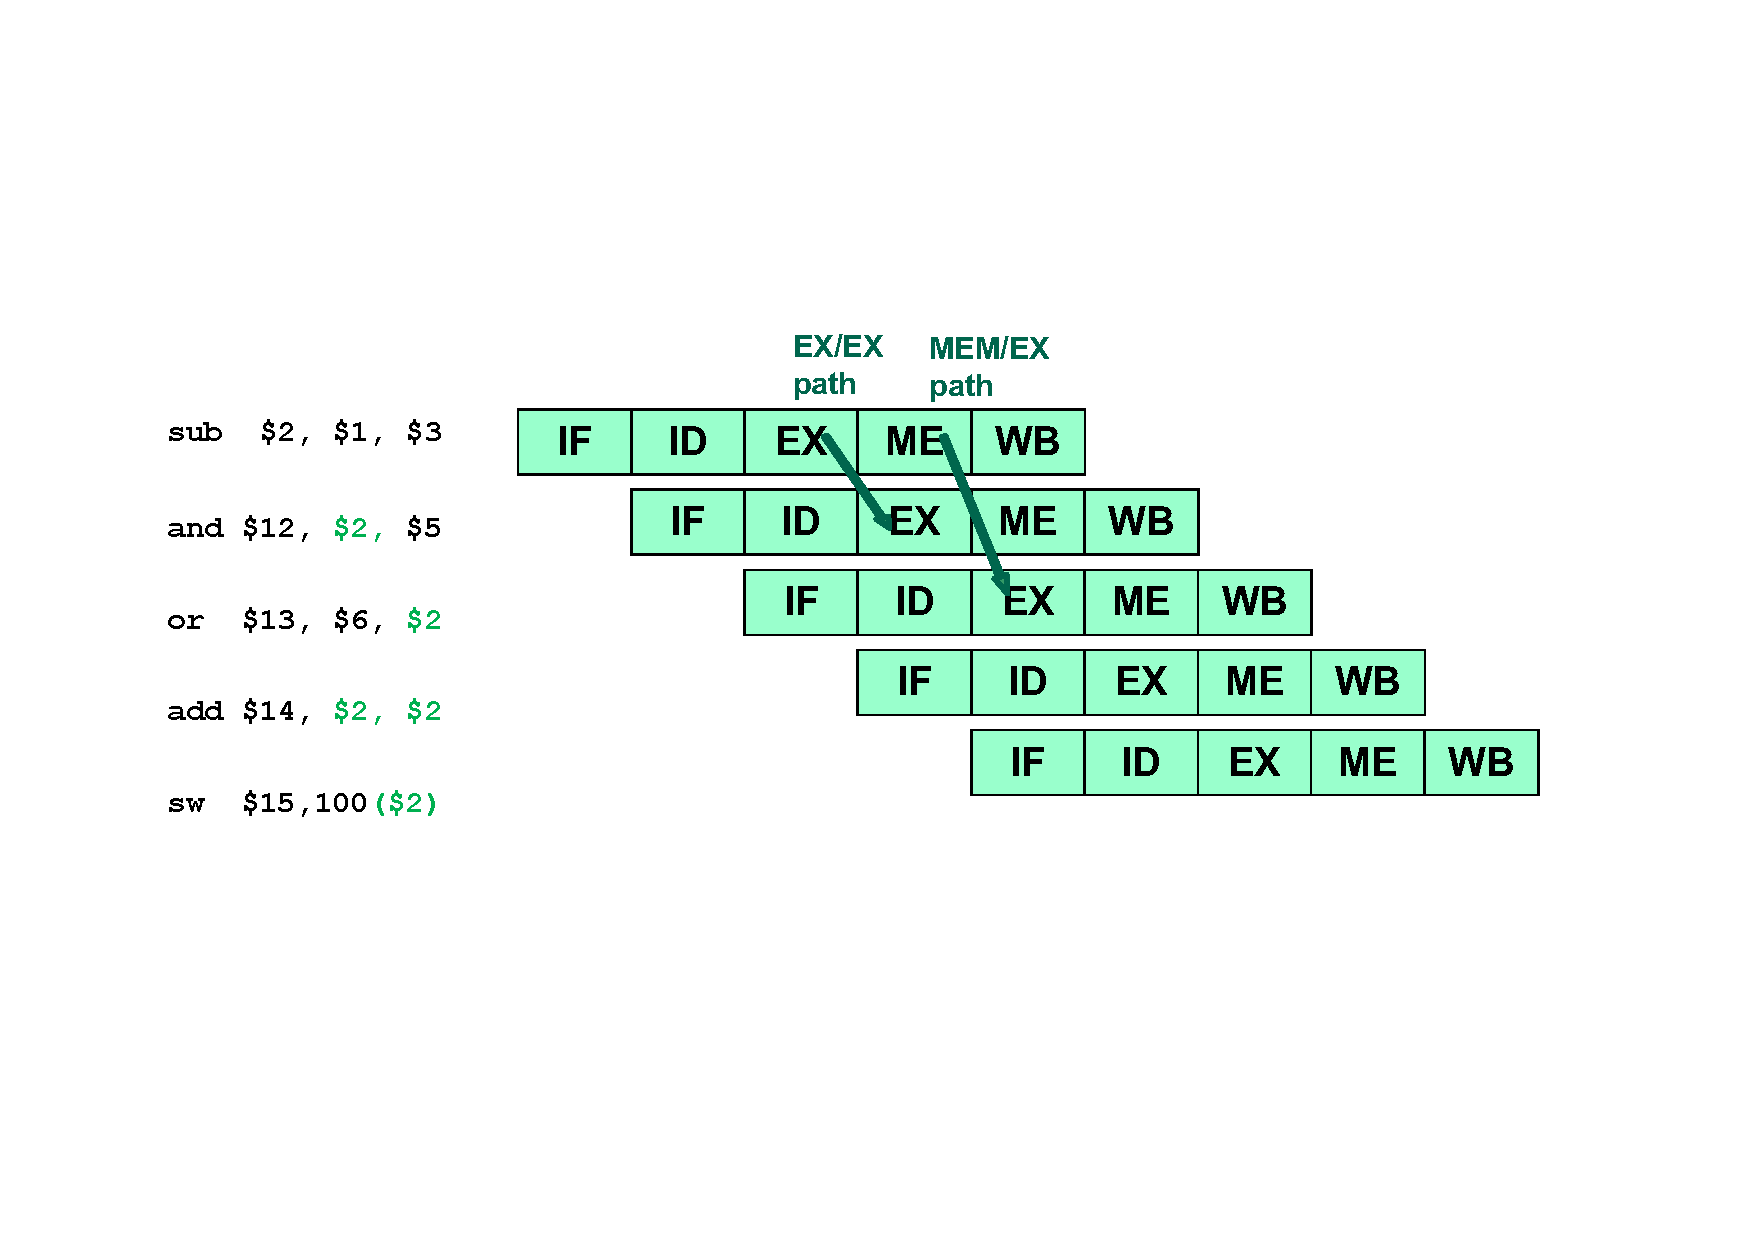
\includegraphics[width=\textwidth]{img/data-forwarding-1.pdf}
        \captionof*{figure}{Data forwarding.\cite{pipelining-slides}}
    \end{center}
\end{examplebox}
    \subsubsection{The solution of Control Hazards}

There are multiple techniques to resolve a Control Hazard.

\begin{flushleft}
    \textcolor{Green3}{\textbf{\faIcon{check} Conservative Solution - The Branch Stalls}}
\end{flushleft}
The following solution is the most conservative. Solve the problem? Yes, but it's called conservative because adopt a banal technique: \textbf{stalling until resolution at the end of the Memory Access} (ME) stage of the branch.

\highspace
The main problem is the \textbf{loss of performance}. Each branch costs a \textbf{penalty of 3 stalls} to decide and fetch the correct instruction flow in the pipeline:
\begin{figure}[!htp]
    \centering
    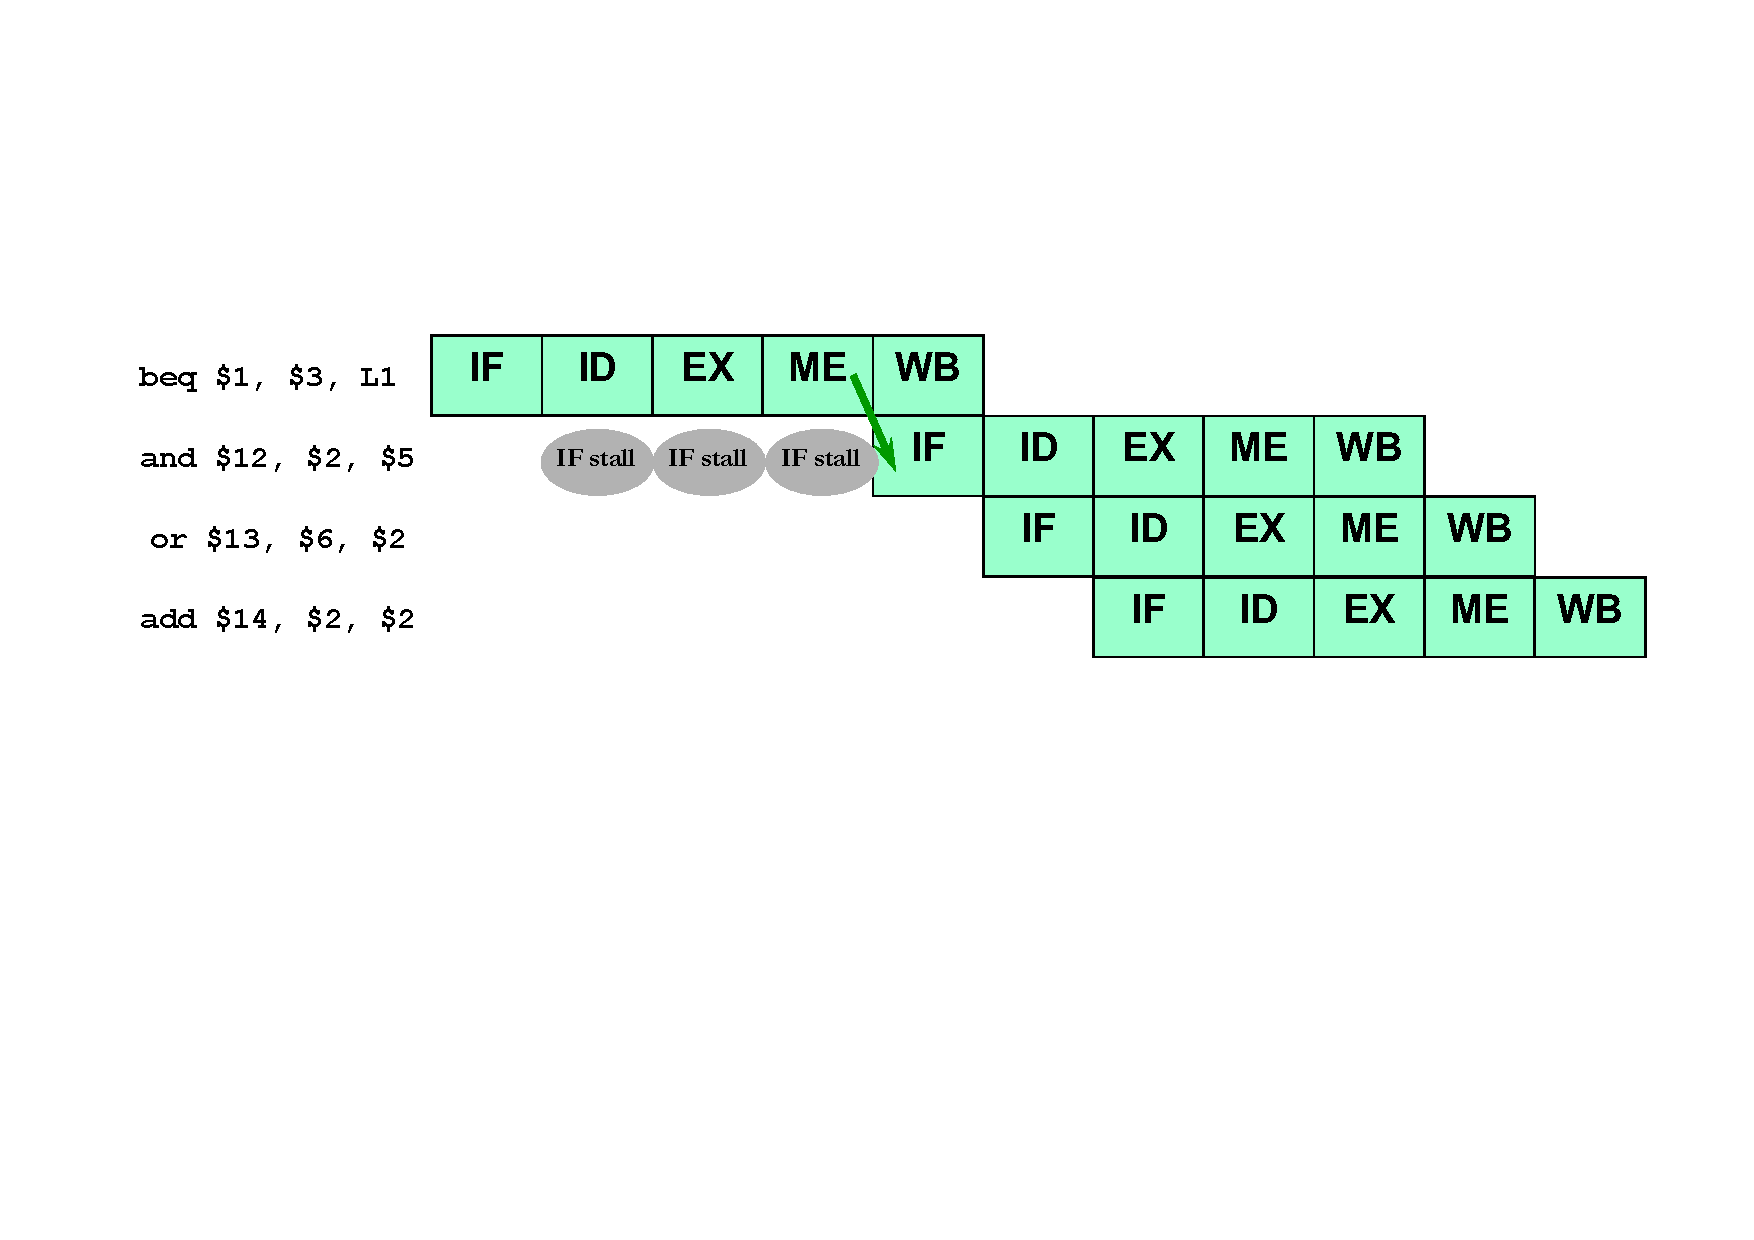
\includegraphics[width=\textwidth]{img/conservative-solution-control-hazards.pdf}
    \caption{\example{Example} of a conservative solution to solve a Control Hazard.}
\end{figure}

\begin{flushleft}
    \textcolor{Green3}{\textbf{\faIcon{check} Start to think to the branch prediction - Flush solution}}
\end{flushleft}
The branch stalls are not good because there is a reduction in throughput. So we can make \emph{a kind of prediction} on the branch and \textbf{assume that the branch will not be taken}. So we start fetching and executing the next 3 instructions in the pipeline. Ok, but wait, \textbf{what if the branch is taken?} No problem, we \textbf{\emph{flush}} the \textbf{next 3 instructions} \underline{before} they write their result and then fetch the instruction at the branch target address.
\begin{figure}[!htp]
    \centering
    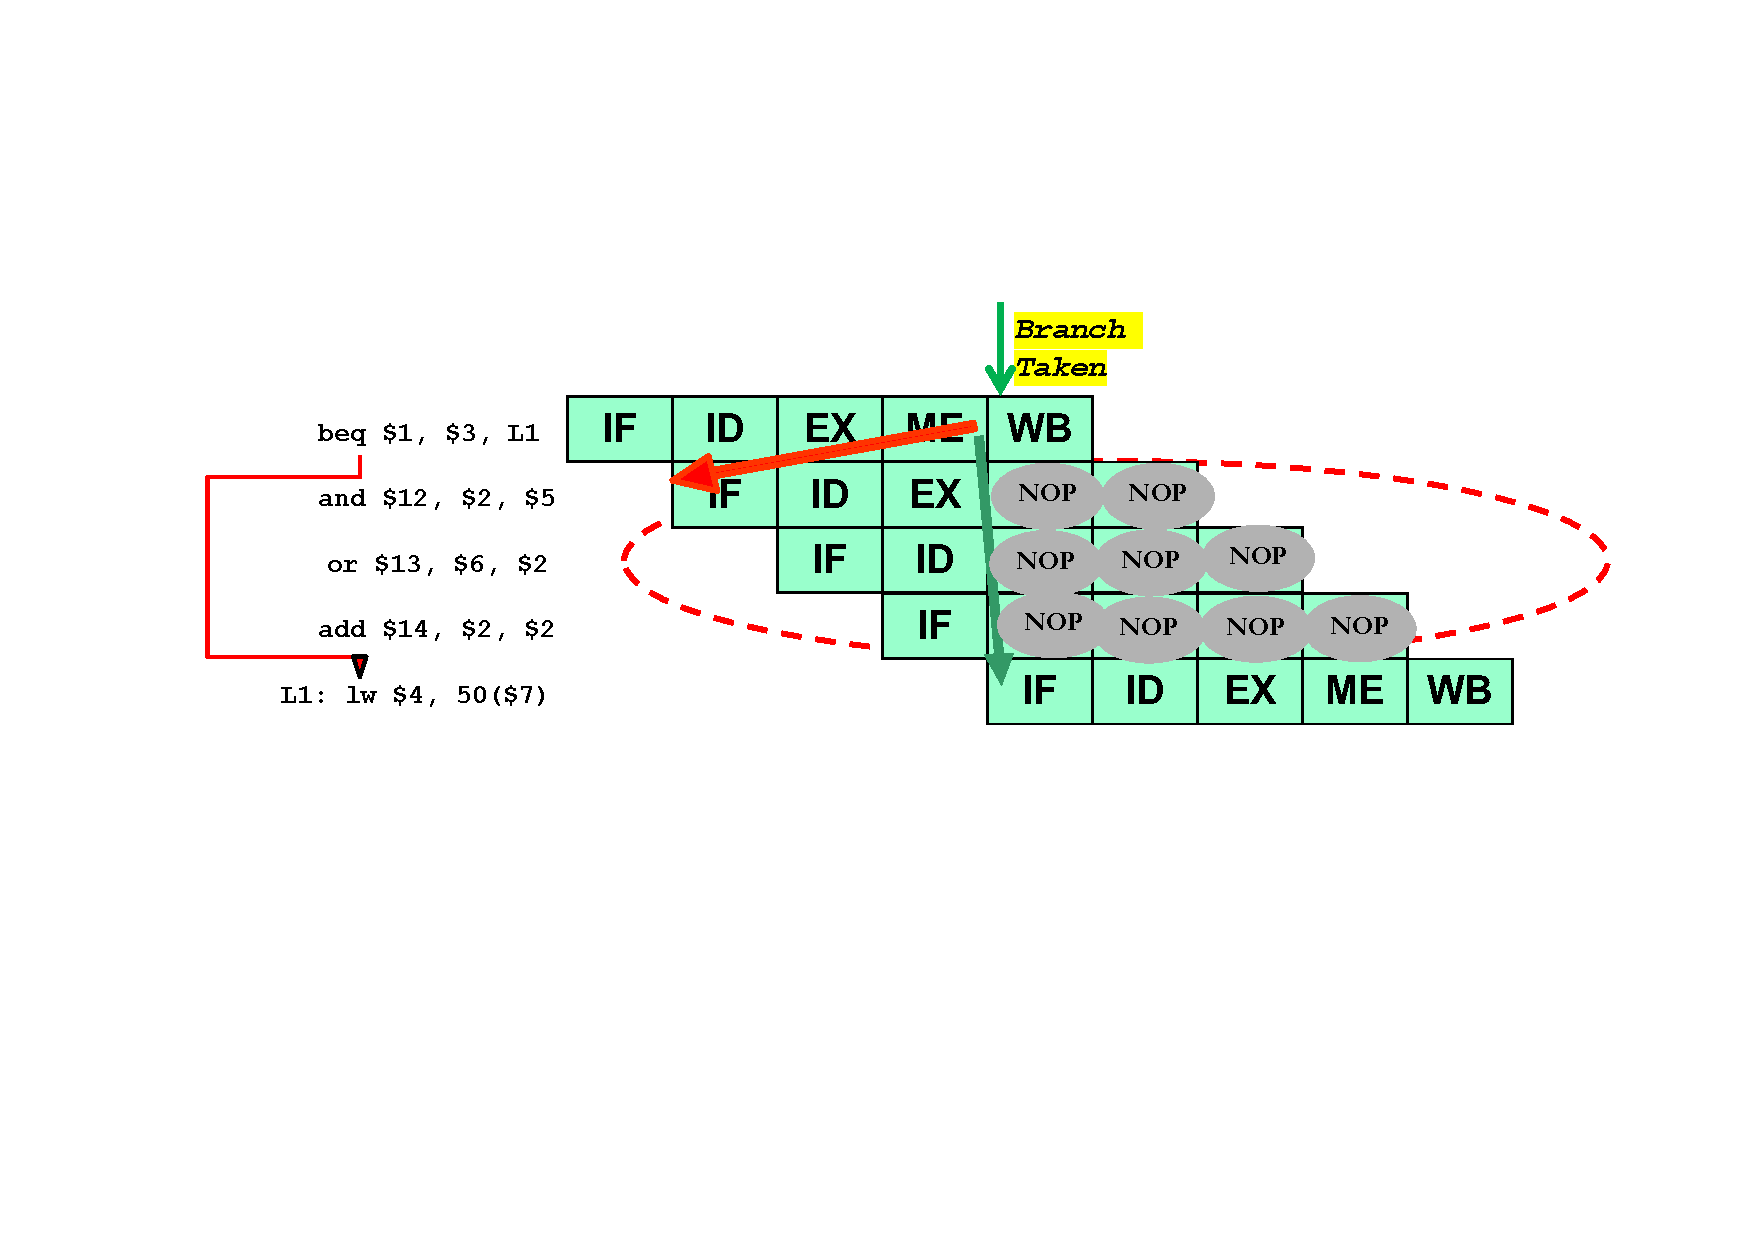
\includegraphics[width=\textwidth]{img/banch-prediciton-control-hazard.pdf}
    \caption{\example{Example} of a flush solution to solve a Control Hazard.}
\end{figure}

\newpage

\begin{flushleft}
    \textcolor{Green3}{\textbf{\faIcon{check} Early Evaluation of the Program Counter (PC) in ID stage}}
\end{flushleft}
It's clear that to improve performance in the event of branch hazards, we need to add more hardware features, such as:
\begin{itemize}
    \item Compare registers to derive the Branch Outcome (BO).
    \item Compute the Branch Target Address (BTA).
    \item Update the PC register.
\end{itemize}
Fortunately, the MIPS-optimized pipeline already has these features and does so during the ID stage. As a result, the \textbf{Branch Outcome} (BO) and the \textbf{Branch Target Address} (BTA) are \textbf{known at the end of the ID stage}.

\begin{figure}[!htp]
    \centering
    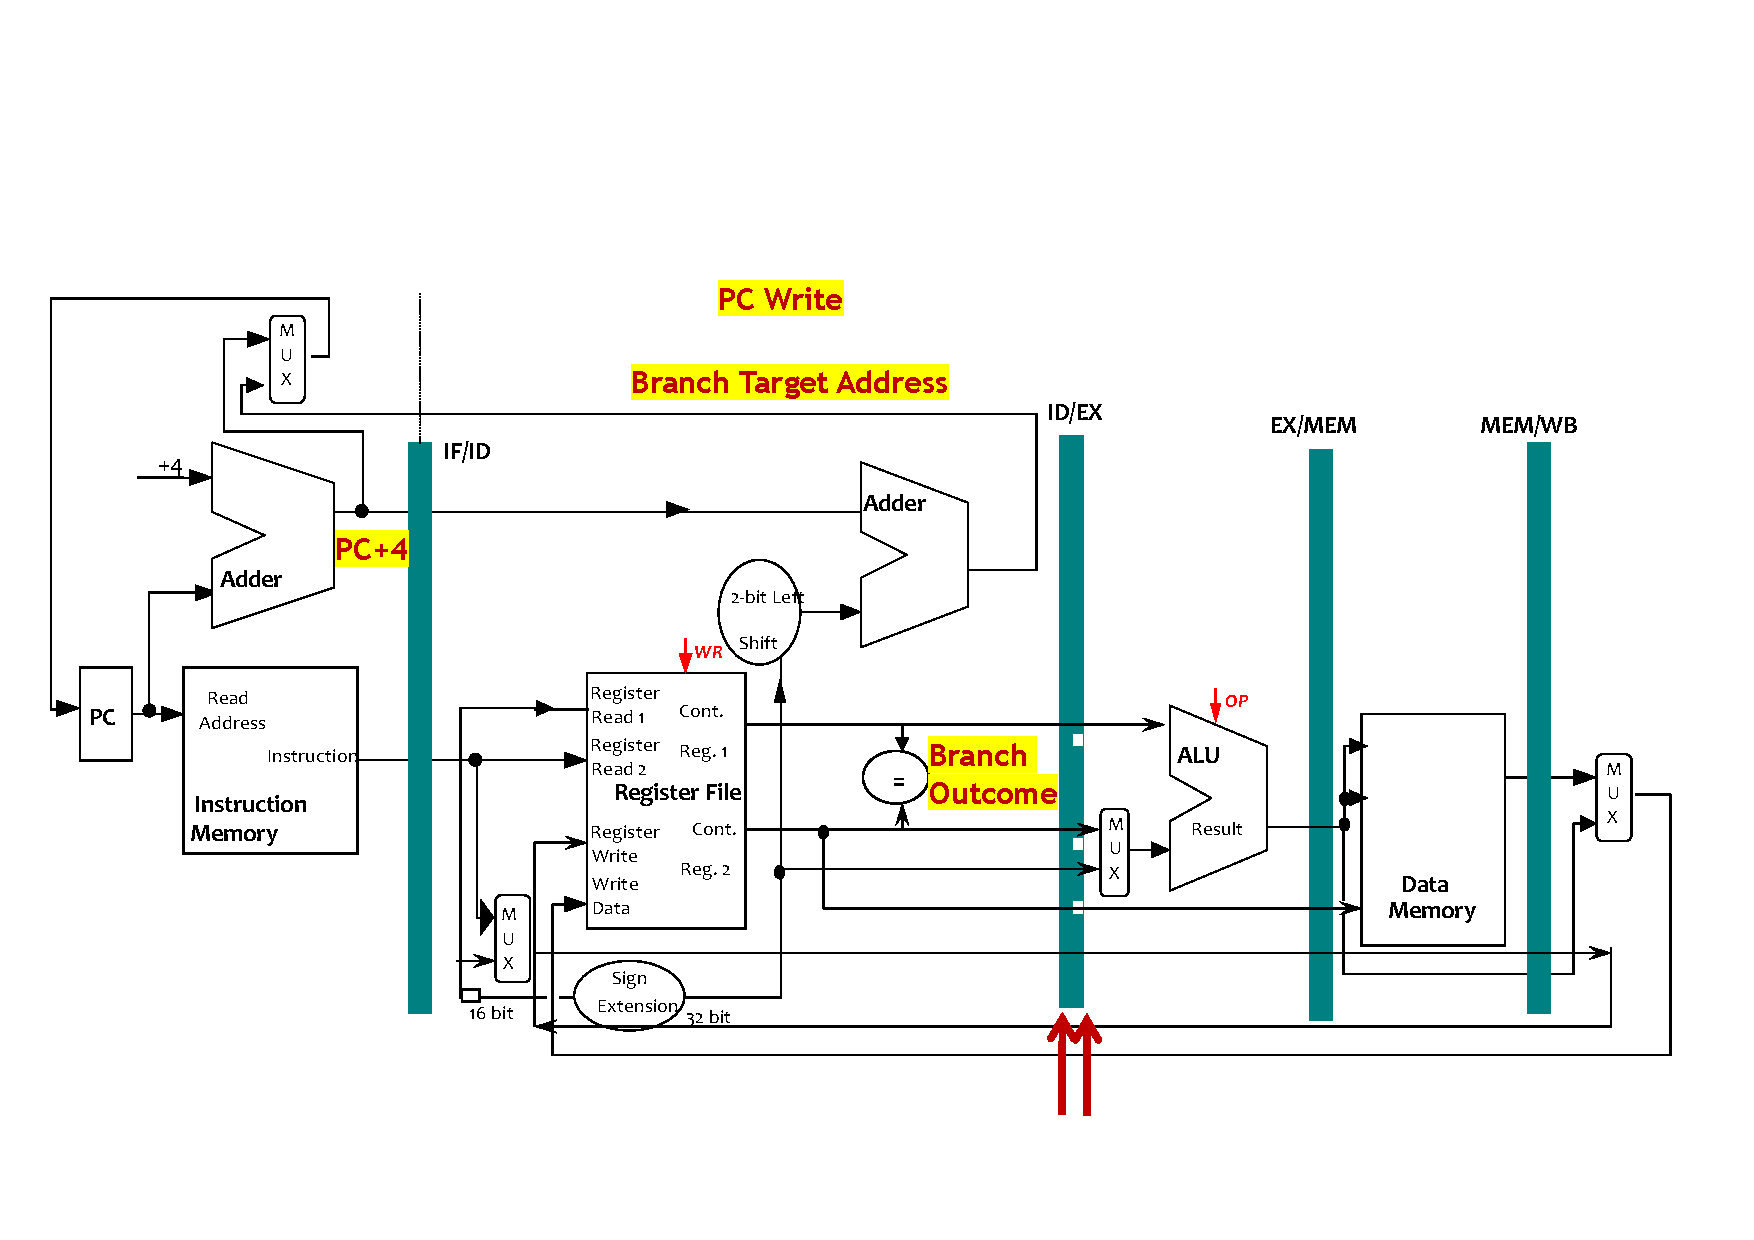
\includegraphics[width=\textwidth]{img/optimization-solution-control-hazard.pdf}
    \caption{Early Evaluation of the Program Counter (PC) in ID stage.}
\end{figure}

\noindent
Now, using the conservative solution or the flush solution, we get two different results:
\begin{itemize}
    \item \textbf{Combo} with \textbf{Conservative Solution}: stalling until resolution at the end of the ID stage (when the Branch Outcome and the Branch Target Address are known) to decide which instruction to fetch.

    \textbf{\emph{Performance consideration}}: each branch costs \textbf{one stall of penalty} to decide and fetch the correct instruction flow along the pipeline.

    One-cycle-delay for every branch still yields a performance loss of 10\% to 30\% depending on the branch frequency (Stall Cycles per Instruction due to Branches equal to Branch Frequency times to Branch Penalty):
    \begin{equation*}
        \texttt{Stall Cycles} = \texttt{Branch Frequency} \times \texttt{Branch Penalty}
    \end{equation*}

    \newpage

    \begin{figure}[!htp]
        \centering
        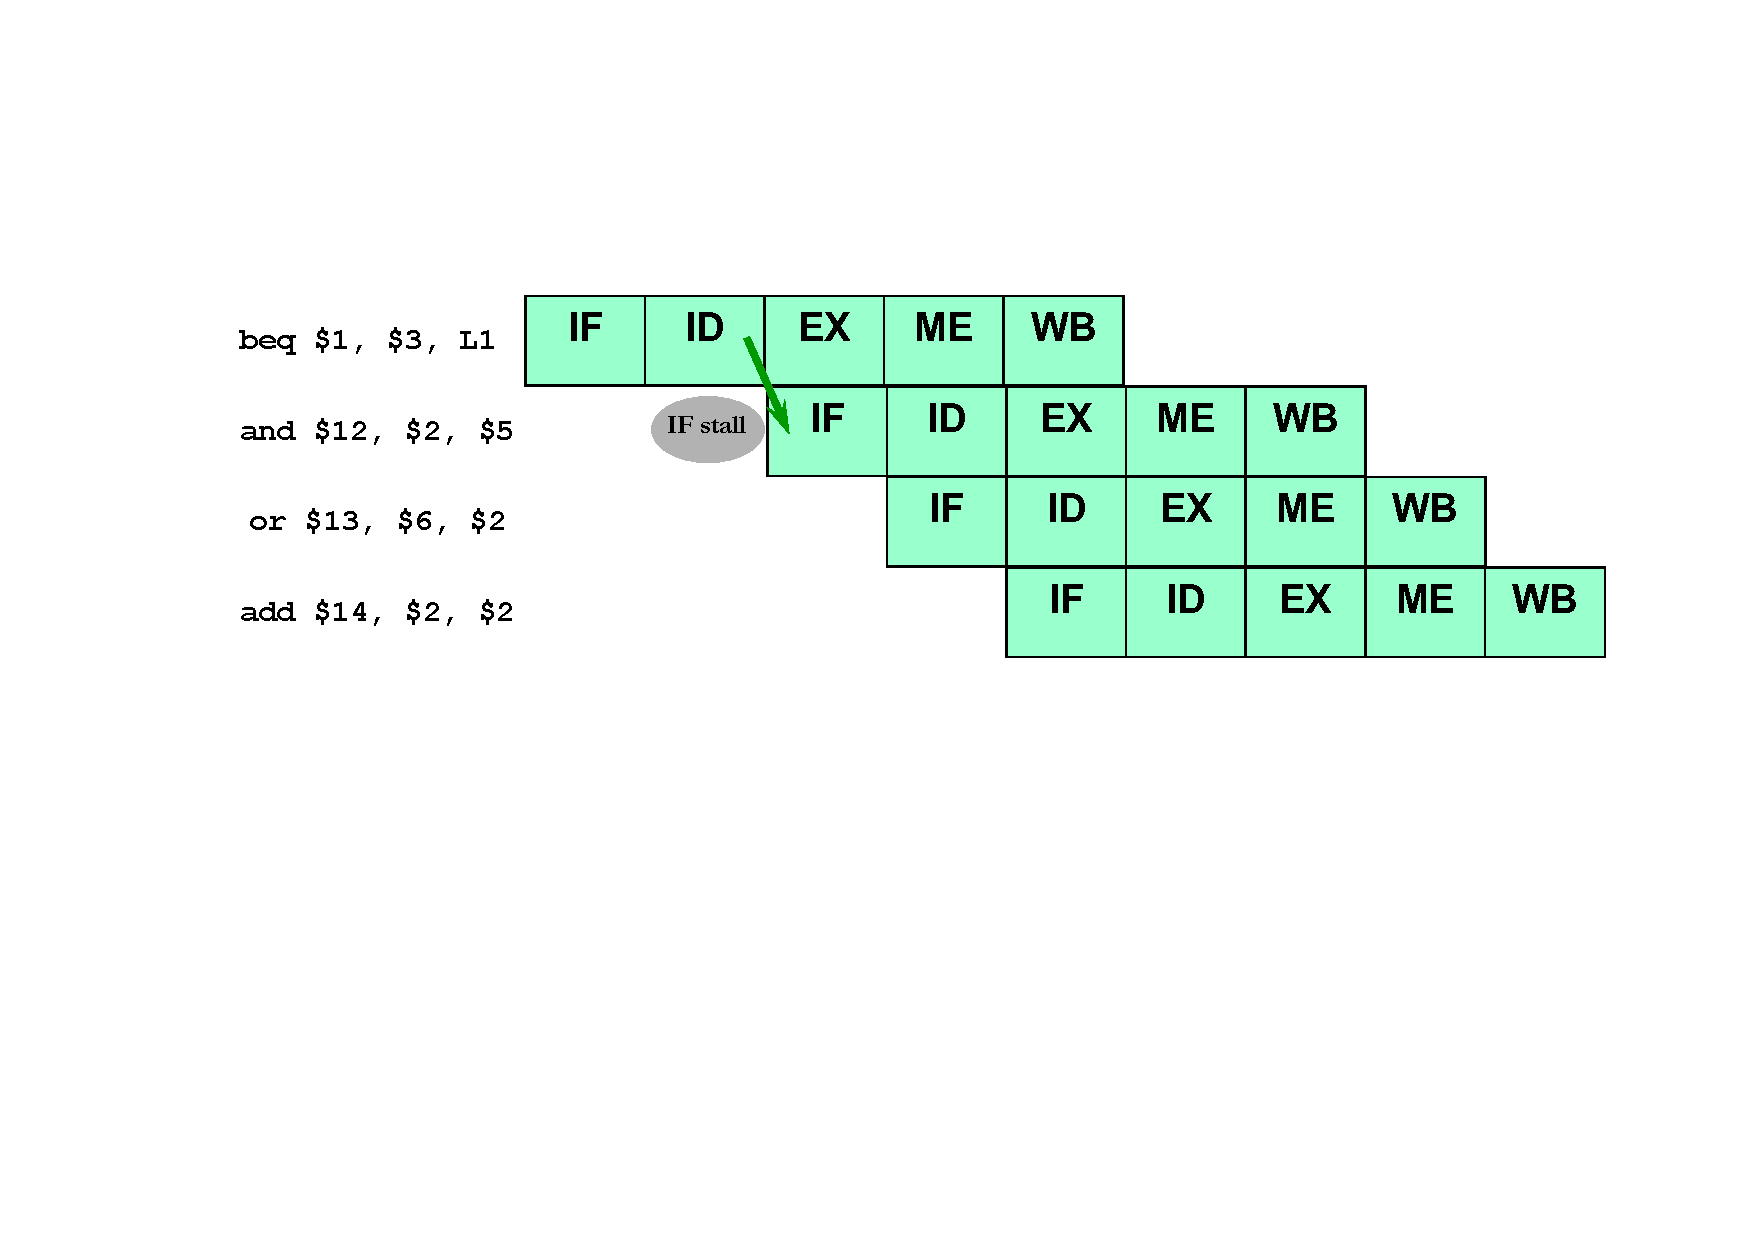
\includegraphics[width=\textwidth]{img/early-evalutation-of-the-pc-1.pdf}
        \caption{\example{Example} of conservative solution in MIPS architecture.}
    \end{figure}

    \item \textbf{Combo} with \textbf{Fetch Solution}: we assume the \textbf{branch is not taken}.
    
    \textbf{\emph{Performance consideration}}: if the Branch Outcome (BO) will be taken, it will be necessary \textbf{to flush only one instructions} before writing its results and fetch the right instruction at the Branch Target Address.
    \begin{figure}[!htp]
        \centering
        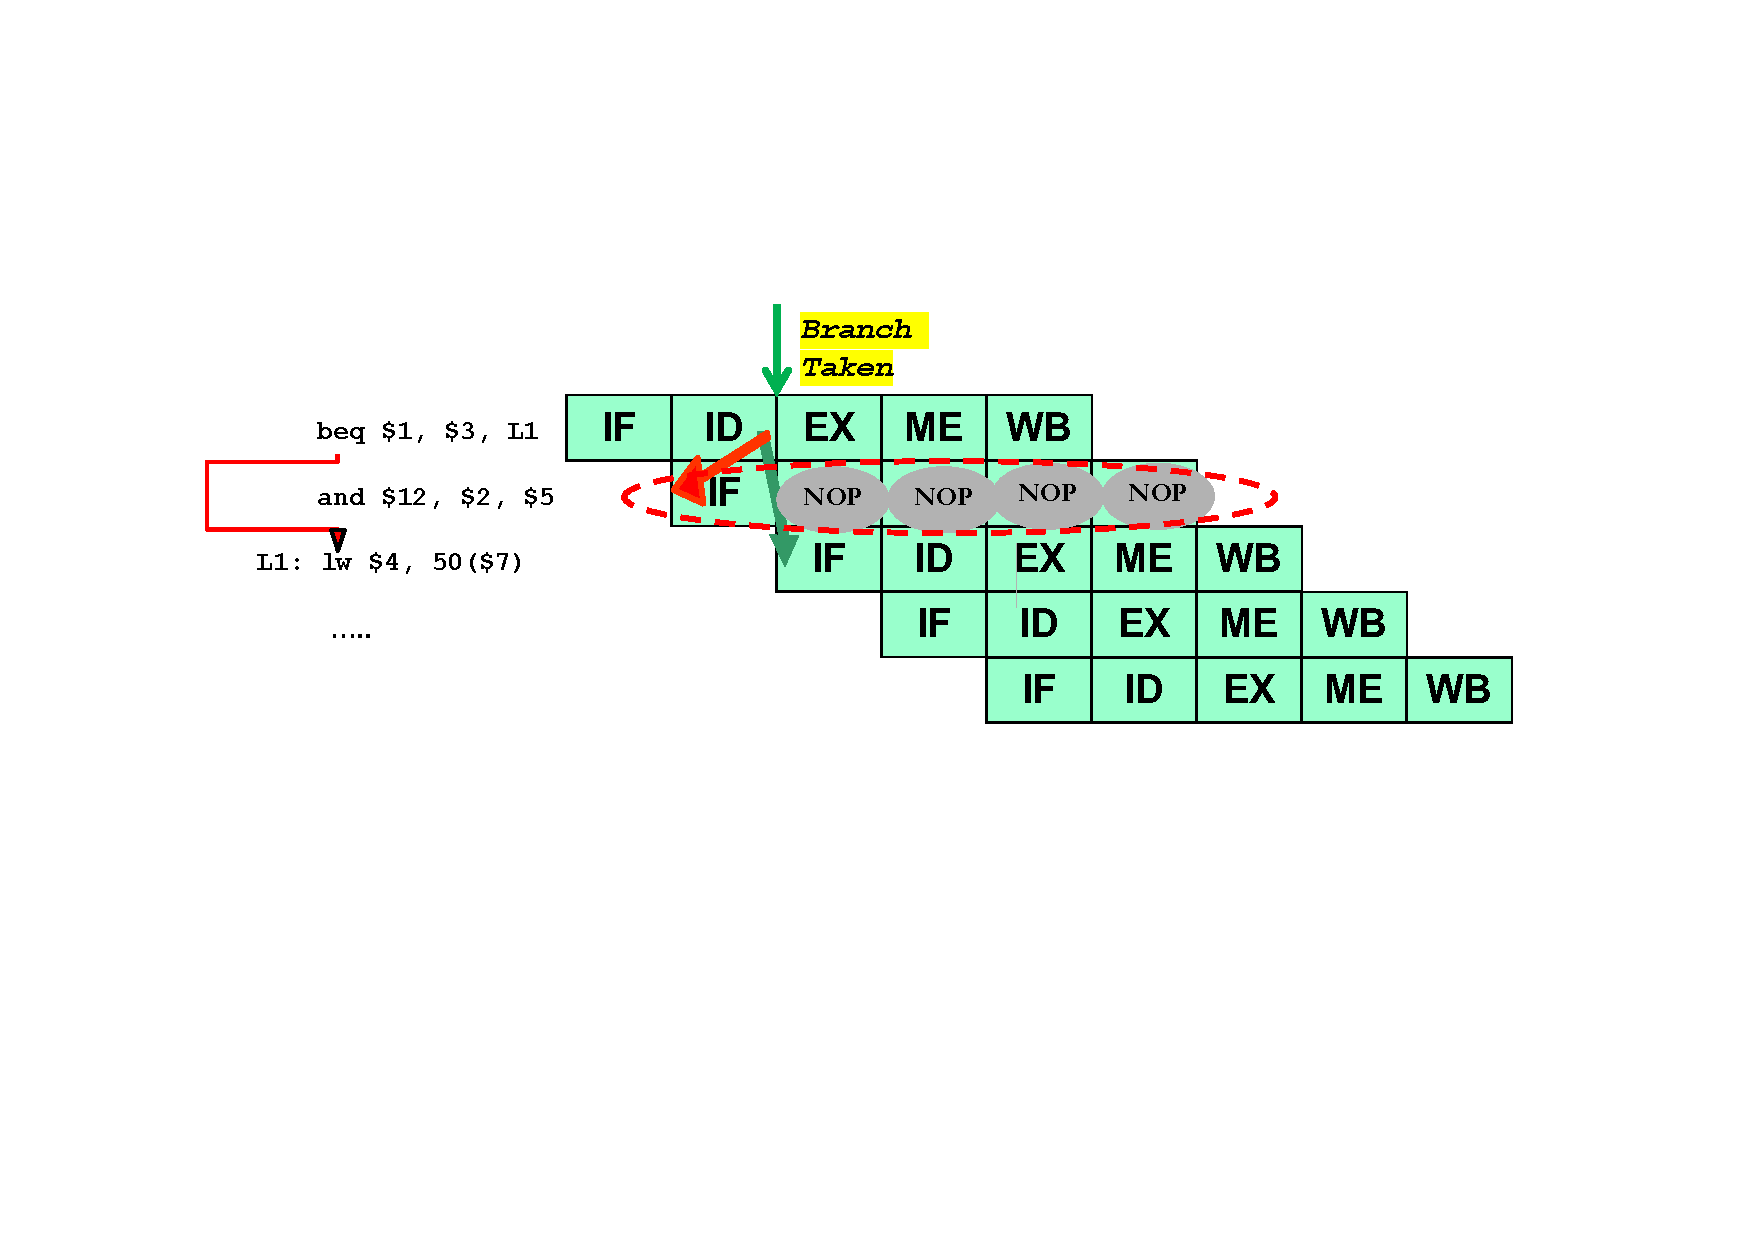
\includegraphics[width=\textwidth]{img/early-evalutation-of-the-pc-2.pdf}
        \caption{\example{Example} of fetch solution in MIPS architecture.}
    \end{figure}
\end{itemize}
The unique solution is to use \textbf{branch prediction techniques} to deal with this loss of performance.
    \subsubsection{Performance evaluation in pipelining}

As we have seen in the previous sections, the \textbf{pipelining increases the CPU instruction throughput} (number of instructions completed per unit of time) but doesn't reduce the latency (the execution time of a single instruction).

\highspace
The \textbf{increase in latency is a direct consequence of two problems}:
\begin{itemize}
    \item The \indexdefinition{imbalance among the pipeline stages}

    \item The \indexdefinition{overhead in the pipeline control}
\end{itemize}
This imbalance between the pipeline stages and the overhead are \underline{bad aspects}:
\begin{itemize}
    \item The \textbf{imbalance} reduces performance because the \textbf{clock can run no faster than the time needed for the slowest pipeline stage};

    \item The \textbf{overhead} arises from the \textbf{delay introduced by interstage registers and clock skew}.
\end{itemize}
Finally, \textbf{all instructions should be the same number of pipeline stages}. Each assumption and optimization shown previously works well in this case.

\begin{definitionbox}[: number of Clock Cycles, Clocks Per Instructions and MIPS formula]
    Given:
    \begin{itemize}
        \item The \textbf{Instruction Count per iteration} as $\texttt{IC}_{\texttt{per\_iter}}$

        \item The \textbf{number of Stall Cycles per iteration} as \texttt{\# Stall Cycles}

        \item The \textbf{length of the pipeline} is $x$
    \end{itemize}
    We can \textbf{calculate the} \indexdefinition{number of Clock Cycles} as the sum between the Instruction Count (how many stages there are in one instruction), the number of Stall Cycles inserted by the hardware technique (called insertion of stalls), plus the length of the pipeline $x$:
    \begin{equation}\label{eq: clock cycles per iteration}
        \texttt{\# Clock Cycles}_{\texttt{per\_iter}} = \texttt{IC}_{\texttt{per\_iter}} + \texttt{\# Stall Cycles}_{\texttt{per\_iter}} + x
    \end{equation}
    The \indexdefinition{Clocks Per Instruction} per iteration, $\texttt{CPI}_{\texttt{per\_iter}}$, is calculated with the rapport between the number of Clock Cycles per iteration (previous equation) divided by the Instruction Count per iteration:
    \begin{equation}\label{eq: clock per instruction per iteration}
        \begin{array}{rcl}
            \texttt{CPI}_{\texttt{per\_iter}} &=& \dfrac{
                \texttt{\# Clock Cycles}_{\texttt{per\_iter}}
            }{
                \texttt{IC}_{\texttt{per\_iter}}
            } \\ \\
            &=& \dfrac{
                \left(\texttt{IC}_{\texttt{per\_iter}} + \texttt{\# Stall Cycles}_{\texttt{per\_iter}} + x\right)
            }{
                \texttt{IC}_{\texttt{per\_iter}}
            }
        \end{array}
    \end{equation}
    Finally, the \indexdefinition{MIPS formula} per iteration is calculated with the rapport between the frequency of the clock ($\texttt{f}_{\texttt{clock}}$) divided by the multiply between the Instructions Per Clock (as the ratio $1 \div \texttt{CPI}$) and $10^{6}$ (1 million instructions):
    \begin{equation}\label{eq: MIPS per iteration}
        \texttt{MIPS}_{\texttt{per\_iter}}
        =
        \dfrac{
            \texttt{f}_{\texttt{clock}}
        }{
            \left(
                \texttt{CPI}_{\texttt{per\_iter}} \times 10^{6}
            \right)
        }
    \end{equation}
\end{definitionbox}

\noindent
We can asymptotically (\texttt{AS}) rewrite equations \ref{eq: clock cycles per iteration}, \ref{eq: clock per instruction per iteration} and \ref{eq: MIPS per iteration} as follows:
\begin{equation}
    \texttt{\# Clock Cycles}_{\texttt{AS}} = \texttt{IC}_{\texttt{AS}} + \texttt{\# Stall Cycles}_{\texttt{AS}} + x
\end{equation}
\vspace{1em}
\begin{equation}
    \begin{array}{rcl}
        \texttt{CPI}_{\texttt{AS}} &=& \lim_{n \rightarrow \infty} \dfrac{
            \texttt{\# Clock Cycles}_{\texttt{AS}}
        }{
            \texttt{IC}_{\texttt{AS}}
        } \\ \\
        &=& \lim_{n \rightarrow \infty} \dfrac{
            \left(
                \texttt{IC}_{\texttt{AS}} + \texttt{\# Stall Cycles}_{\texttt{AS}} + x
            \right)
        }{
            \texttt{IC}_{\texttt{AS}}
        }
    \end{array}
\end{equation}
\vspace{1em}
\begin{equation}
    \texttt{MIPS}_{\texttt{AS}} = \dfrac{
        \texttt{f}_{\texttt{clock}}
    }{
        \left(\texttt{CPI}_{\texttt{AS}} \times 10^{6}\right)
    }
\end{equation}
Note: the \textbf{ideal speedup, then Clock Per Instruction, should be equal to 1}. But stalls cause the pipeline performance to degrade from the ideal performance, so we have the \indexdefinition{Average Clock Per Instruction (CPI)}:
\begin{equation}
    \begin{array}{rcl}
        \texttt{AVG}\left(\texttt{CPI}\right) &=& \texttt{Ideal CPI} + \texttt{\# Stall Cycles}_{\texttt{per\_instruction}} \\ \\
        &=& 1 + \texttt{\# Stall Cycles}_{\texttt{per\_instruction}}
    \end{array}
\end{equation}
And obviously, the \indexdefinition{Pipeline Stall Cycles per Instruction} is:
\begin{equation}
    \texttt{PSCI} = \texttt{Structural Haz.} + \texttt{Data Haz.} + \texttt{Control Haz.} + \texttt{Memory Stalls}
\end{equation}
    \section{Software Configuration Management}

\subsection{Introduction}

\href{https://www.atlassian.com/microservices/microservices-architecture/configuration-management}{Configuration Management (CM)} is a systems engineering process for establishing consistency of a product's attributes throughout its life. In the technology world, configuration management is an IT management process that tracks individual configuration items of an IT system. IT systems are composed of IT assets that vary in granularity. An IT asset may represent a piece of software, or a server, or a cluster of servers. The following focuses on configuration management as it directly applies to IT software assets and software asset CI/CD.

\highspace
\definition{Software Configuration Management} is a \textbf{systems engineering process that tracks and monitors changes to a software systems configuration metadata}. In software development, configuration management is commonly used alongside version control and CI/CD infrastructure (explained later).

\highspace
The basic \textbf{approach to using a decentralized CM} is to have a repository (project) on the server side. 
\begin{itemize}
    \item When we want to work on the project, we clone the repository on the local PC. This workflow is used because we can work offline and on the local project without making critical changes to the repository server side.
    
    \item The local changes can be saved using the commit command and when we are ready to publish our changes, we use the push command to update the repository on the server side.
    
    \item After a push, anyone who has a local copy should make a pull command to update the local project.
\end{itemize}
This workflow can be done using git commands, and a good cheat sheet can be found \href{https://education.github.com/git-cheat-sheet-education.pdf}{here}.
    \subsubsection{Cache Hit and Cache Miss}

Unfortunately, the Cache can't be maintain every data inside the computer. In order to be faster, it contains only some data with.

\highspace
When the processor makes a request of a certain type:
\begin{itemize}
    \item \textcolor{Green3}{\textbf{\emph{Ideal case}}}. If the \textbf{requested data is \underline{found} in one of the cache blocks} (upper level), then there is a hit in the cache address and it's called \indexdefinition{Cache Hit}.

    \item \textcolor{Red2}{\textbf{\emph{Problematic case}}}. If the \textbf{requested data is \underline{not found} in one of the cache blocks} (upper level), then there is a miss in the cache address and it's called \indexdefinition{Cache Miss}.

    \underline{But beware}, in this case we need to access the lower level of the memory hierarchy to find the requested block. This causes:
    \begin{itemize}
        \item \textbf{To stall the CPU};
        \item To require to block from the main memory;
        \item To copy (write) the block in cache;
        \item To repeat the cache access (hit).
    \end{itemize}
\end{itemize}

\begin{definitionbox}[: Cache Hit]\label{definition: Cache Hit}
    A \indexdefinition{Cache Hit} is when a requested data is found in one of the cache block of the upper level of the memory.
\end{definitionbox}

\noindent
Furthermore we define the \indexdefinition{Hit Rate} as the \textbf{number of memory accesses that find the data in the upper level with respect to the total number of memory accesses}:
\begin{equation*}
    \texttt{Hit Rate} = \dfrac{\texttt{\# hits}}{\texttt{\# memory accesses}}
\end{equation*}
Finally we define the \indexdefinition{Hit Time} as the \textbf{time to access the data in the upper level of the hierarchy}, \textbf{including the time needed to decide} if the attempt of access will result in a hit or miss.


\begin{definitionbox}[: Cache Miss]\label{definition: Cache Miss}
    A \indexdefinition{Cache Miss} is when a requested data is not found in one of the cache blocks and must be taken from the lower level of the memory.
\end{definitionbox}

\noindent
Furthermore we define the \indexdefinition{Miss Rate} as the \textbf{number of memory accesses not finding the data in the upper level with respect to the total number of memory accesses}:
\begin{equation}\label{eq: Miss Rate}
    \texttt{Miss Rate} = \dfrac{\texttt{\# misses}}{\texttt{\# memory accesses}}
\end{equation}
Finally we define the \indexdefinition{Miss Time} as
\begin{equation}\label{eq: Miss Time}
    \texttt{Miss Time} = \texttt{Hit Time} + \texttt{Miss Penalty}
\end{equation}
Where the \indexdefinition{Miss Penalty} is \textbf{the time needed to access the lower level and to replace the block in the upper level}.

\highspace
Two observations:
\begin{enumerate}
    \item Should be obviously the definition:
    \begin{equation*}
        \texttt{Hit Rate} + \texttt{Miss Rate} = 1
    \end{equation*}

    \item Typically, we have the following relation:
    \begin{equation*}
        \texttt{Hit Time} \ll \texttt{Miss Penalty}
    \end{equation*}
\end{enumerate}
Finally, the \indexdefinition{Average Memory Access Time (AMAT)} can be calculated as:
\begin{equation}\label{eq: Average Memory Access Time (AMAT)}
    \texttt{AMAT} = \texttt{Hit Time} + \texttt{Miss Rate} * \texttt{Miss Penalty}
\end{equation}
    \subsubsection{Cache Structure}

Each entry (cache line) in the cache includes:
\begin{itemize}
    \item (\textbf{V}) \textbf{Valid bit} to indicate if this position contains valid data or not. At the bootstrap, all the entries in the cache are marked as \texttt{INVALID}.

    \item (\textbf{TAG}) \textbf{Cache Tag(s)} contains the value that univocally identifies the memory address corresponding to the stored data.

    \item (\textbf{DATA}) \textbf{Cache Data} contains a copy of data (block or cache line).
\end{itemize}
\begin{figure}[!htp]
    \centering
    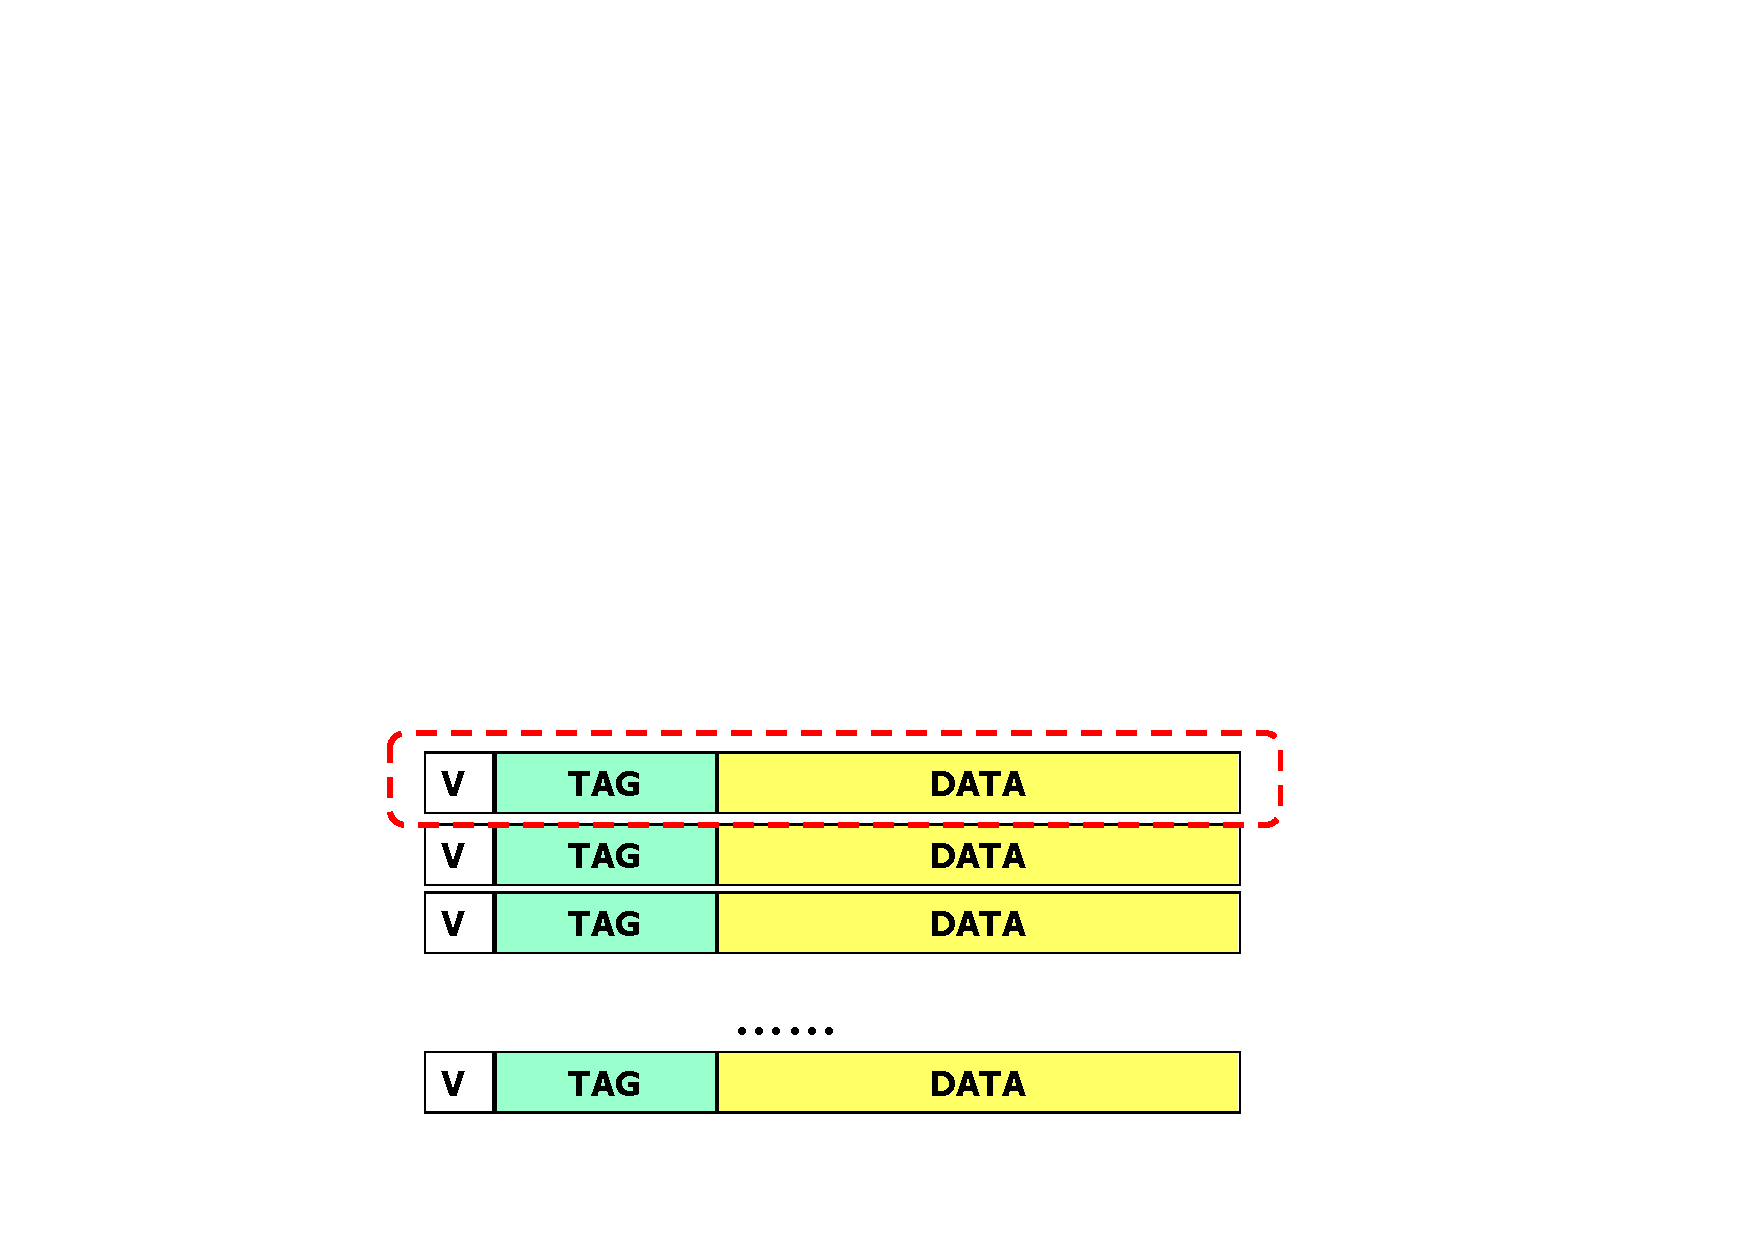
\includegraphics[width=.7\textwidth]{img/cache-structure-1.pdf}
\end{figure}

\noindent
After a general presentation of the cache structure, we answer four questions about the memory hierarchy to understand different topics: 
\begin{itemize}
    \item \textbf{Block placement} (page~\hyperlink{Block placement}{\hypergetpageref{Block placement}}). \emph{Where can a block be placed in the upper level?}
    \begin{itemize}
        \item Direct Mapped Cache (page~\hyperlink{Direct Mapped Cache}{\hypergetpageref{Direct Mapped Cache}})

        \item Fully Associative Cache (page~\hyperlink{Fully Associative Cache}{\hypergetpageref{Fully Associative Cache}})
        
        \item \emph{n}-way Set Associative Cache (page~\hyperlink{n-way Set Associative Cache}{\hypergetpageref{n-way Set Associative Cache}})
    \end{itemize}
    
    \item \textbf{Block identification} (page~\hyperlink{Block identification}{\hypergetpageref{Block identification}}). \emph{How is a block found if it is in the upper level?}
    
    \item \textbf{Block replacement} (page~\hyperlink{Block replacement}{\hypergetpageref{Block replacement}}). \emph{Which block should be replaced on a miss?}
    
    \item \textbf{Write strategy} (page~\hyperlink{Write strategy}{\hypergetpageref{Write strategy}}). \emph{What happens on a write?}
\end{itemize}

\newpage

\begin{center}
    \large
    \label{Block placement}
    \hypertarget{Block placement}{\textcolor{Red2}{\textbf{Block placement}}}
\end{center}

\noindent
The main question is: \emph{where can a block be placed in the upper level?} In other words, the problem is: given the address of the block in the main memory, \textbf{where can the block be placed in the cache}?

\highspace
So, we need to find the \textbf{correspondence between the memory address and the cache address of the block}. This correspondence \textbf{depends on the cache structure} and can be of three types:
\begin{itemize}
    \item \textbf{Direct Mapped Cache}
    \item \textbf{Fully Associative Cache}
    \item \textbf{\emph{n}-way Set-Associative Cache}
\end{itemize}

\label{Direct Mapped Cache}
\hypertarget{Direct Mapped Cache}{\subsubsection*{\textcolor{Red2}{Direct Mapped Cache}}}

With the \definition{Direct Mapped Cache} structure, \textbf{each memory location corresponds to one cache location and only one cache location}. The following formula gives the \textbf{cache address of the block}:
\begin{equation}\label{eq: direct mapped cache}
    \left(\texttt{Block Address}\right)_{\texttt{cache}} = \left(\texttt{Block Address}\right)_{\texttt{mem}} \texttt{mod} \left(\texttt{\# Cache Blocks}\right)
\end{equation}
The \emph{block address} of the \emph{cache} corresponds to the modulo operation between the \emph{block address} of the \emph{memory} and the \emph{number} (\#) \emph{of cache blocks}. The \href{https://en.wikipedia.org/wiki/Modulo}{modulo operation} returns a division's remainder or signed remainder after dividing one number by another.

\begin{figure}[!htp]
    \centering
    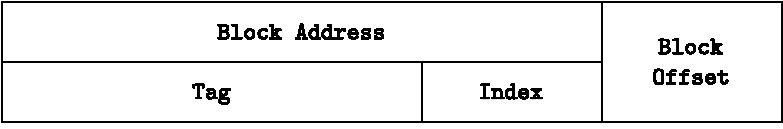
\includegraphics[width=.9\textwidth]{img/direct-mapped-cache-1.pdf}
    \caption{This figure shows the memory address composed of the block address (tag and index used to identify the block) and the block offset.}
    \label{fig: Memory Address - Direct Mapped Cache}
\end{figure}

\noindent
From Figure~\ref{fig: Direct Mapped Cache - Structure}, we can see the complete structure of the cache if we choose the direct mapped cache technique. 

\highspace
The rectangle on the top is the memory address (Figure~\ref{fig: Memory Address - Direct Mapped Cache}). First, we check the \emph{Tag} value; if it's equal to the value in the cache, we check the \emph{Valid bit} (V) to see if the position contains valid data: if the value is 1, we have a cache hit; otherwise, the data is invalid. The \emph{Tag} contains the value that univocally identifies the memory address corresponding to the stored data. To take the \emph{data word}, we use the \emph{block offset} as the \emph{selector} in the \href{https://en.wikipedia.org/wiki/Multiplexer}{multiplexer} to choose which data block to take. The index field indicates the cache row to check.

\newpage

\begin{figure}[!htp]
    \centering
    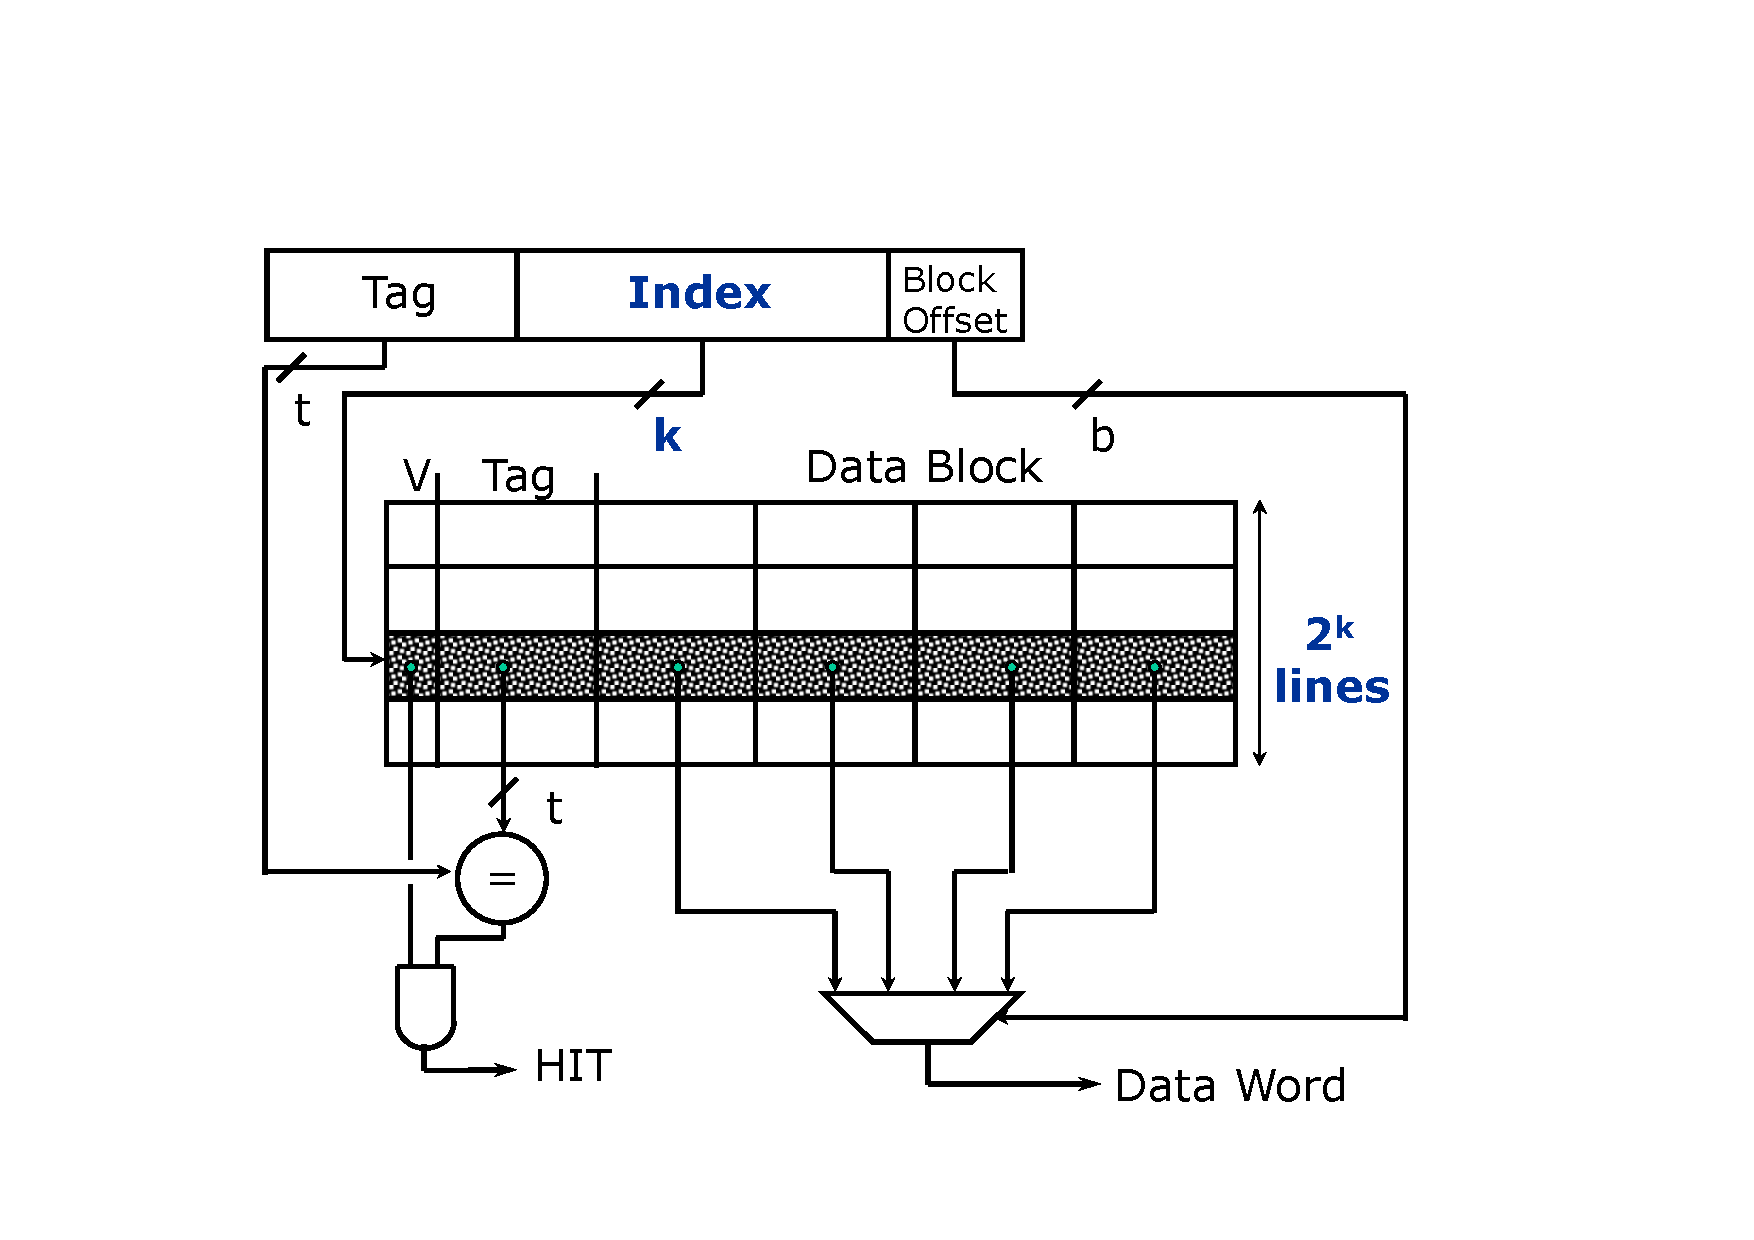
\includegraphics[width=.7\textwidth]{img/direct-mapped-cache-2.pdf}
    \caption{The cache structure of the \emph{Direct Mapped Cache} technique.}
    \label{fig: Direct Mapped Cache - Structure}
\end{figure}

\noindent
For \example{example}, we assume a block-frame address composed of 32 bits. Our cache structure is direct mapped, and the number of cache blocks is 8. A possible exercise could be \textbf{determining where block 12 can be placed in the 8-block cache}.

\highspace
To solve this problem, we can use the formula no \ref{eq: direct mapped cache} on page \pageref{eq: direct mapped cache}: 
\begin{equation*}
    \left(\texttt{Block Address}\right)_{\texttt{cache}} = 12 \mod 8 = 5
\end{equation*}
The result is $5$, so the answer is: with the direct mapped technique, \textbf{the block number is 4} (because the first index of the cache blocks is zero and not 1).

\begin{figure}[!htp]
    \centering
    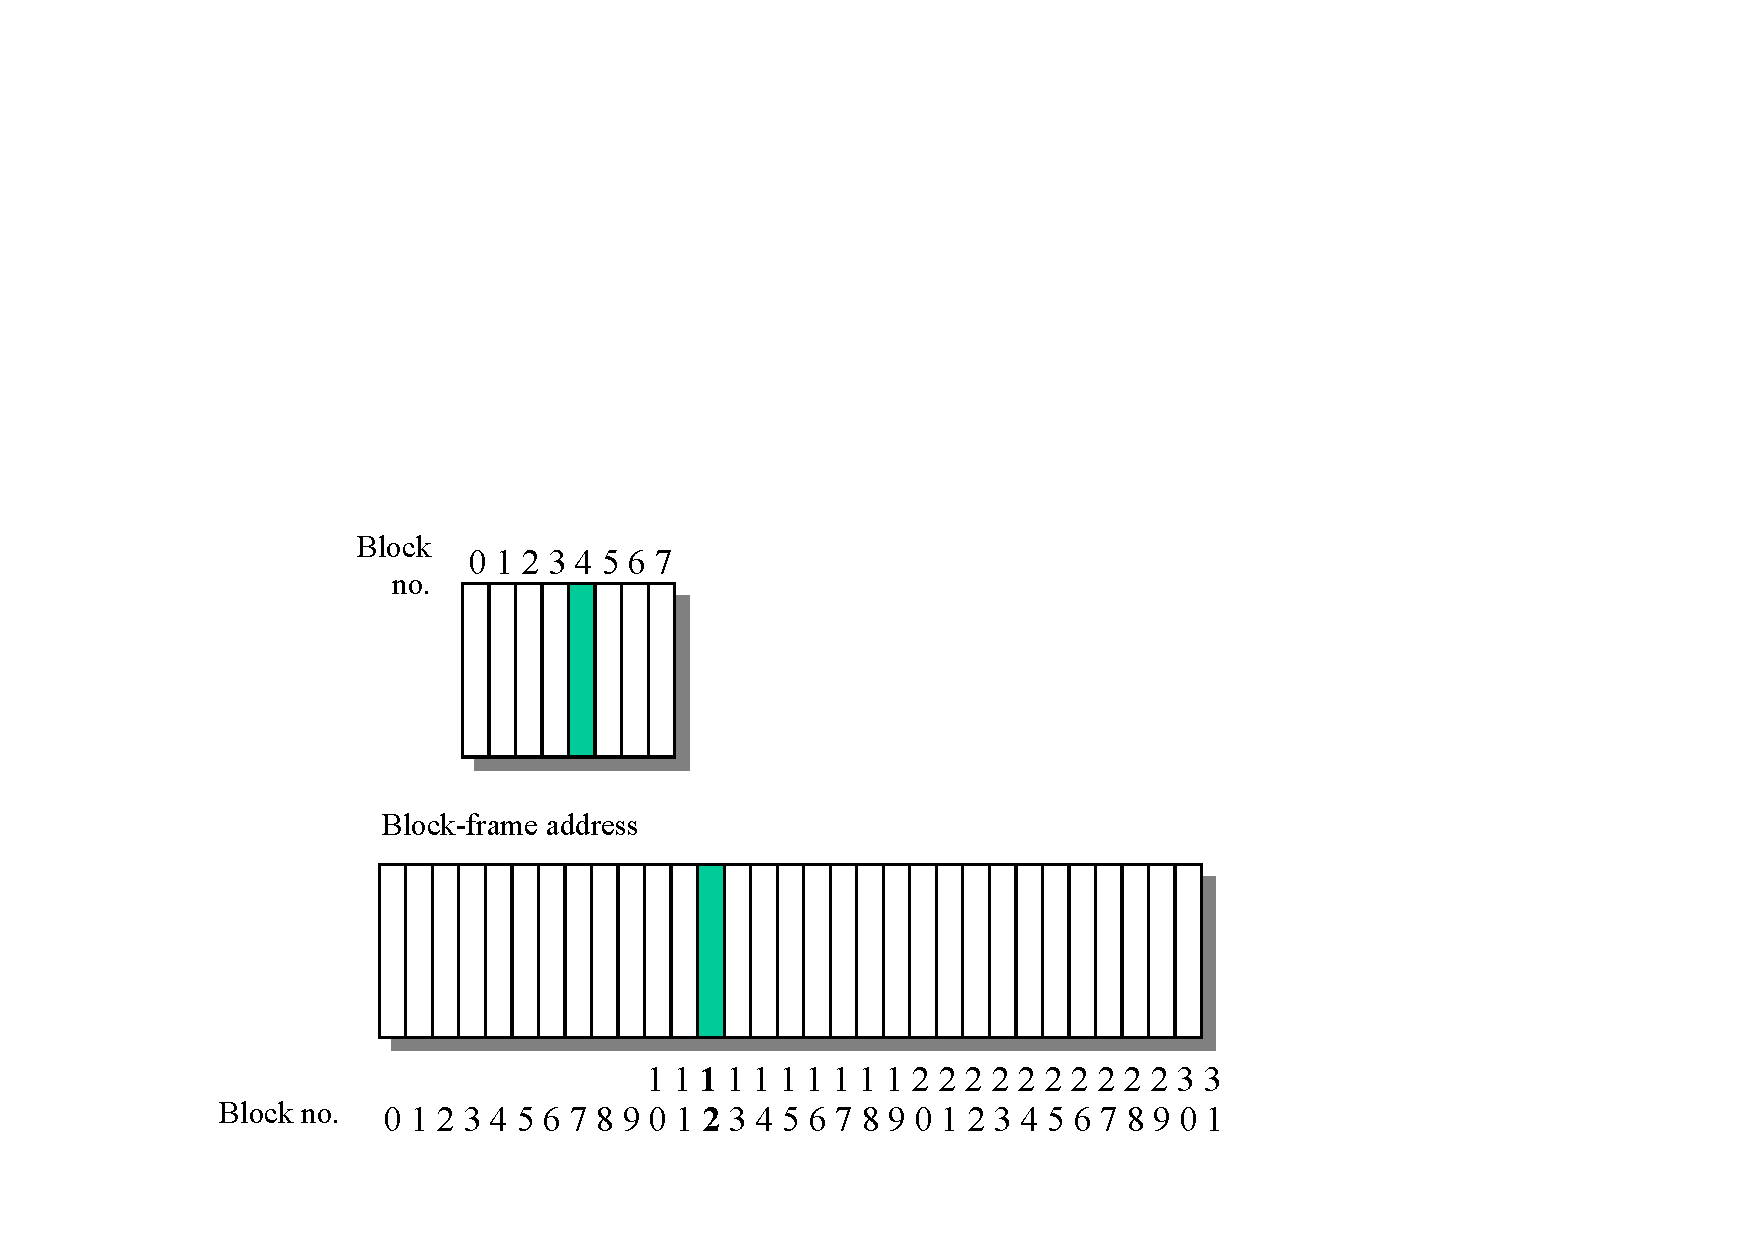
\includegraphics[width=.8\textwidth]{img/direct-mapped-cache-3.pdf}
\end{figure}

\newpage

\label{Fully Associative Cache}
\hypertarget{Fully Associative Cache}{\subsubsection*{\textcolor{Red2}{Fully Associative Cache}}}

In a \definition{Fully Associative Cache}, the \textbf{memory block can be placed in any position of the cache}. So, all the \textbf{cache blocks must be checked during the search of the block}.

\highspace
Note the \textbf{index does not exist} in the memory address; there are the Tag bits only:
\begin{equation}\label{eq: Fully Associative Cache}
    \texttt{Number of blocks} = \dfrac{\texttt{Cache Size}}{\texttt{Block Size}}
\end{equation}
The Memory Address comprises the Block Address (Tag) and the Block Offset.

\begin{figure}[!htp]
    \centering
    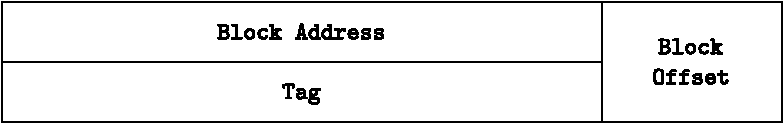
\includegraphics[width=.9\textwidth]{img/fully-associative-cache-1.pdf}
    \caption{The Memory Address comprises the Block Address (Tag) and the Block Offset.}
\end{figure}

\noindent
The structure of the cache using this technique is as follows:

\begin{figure}[!htp]
    \centering
    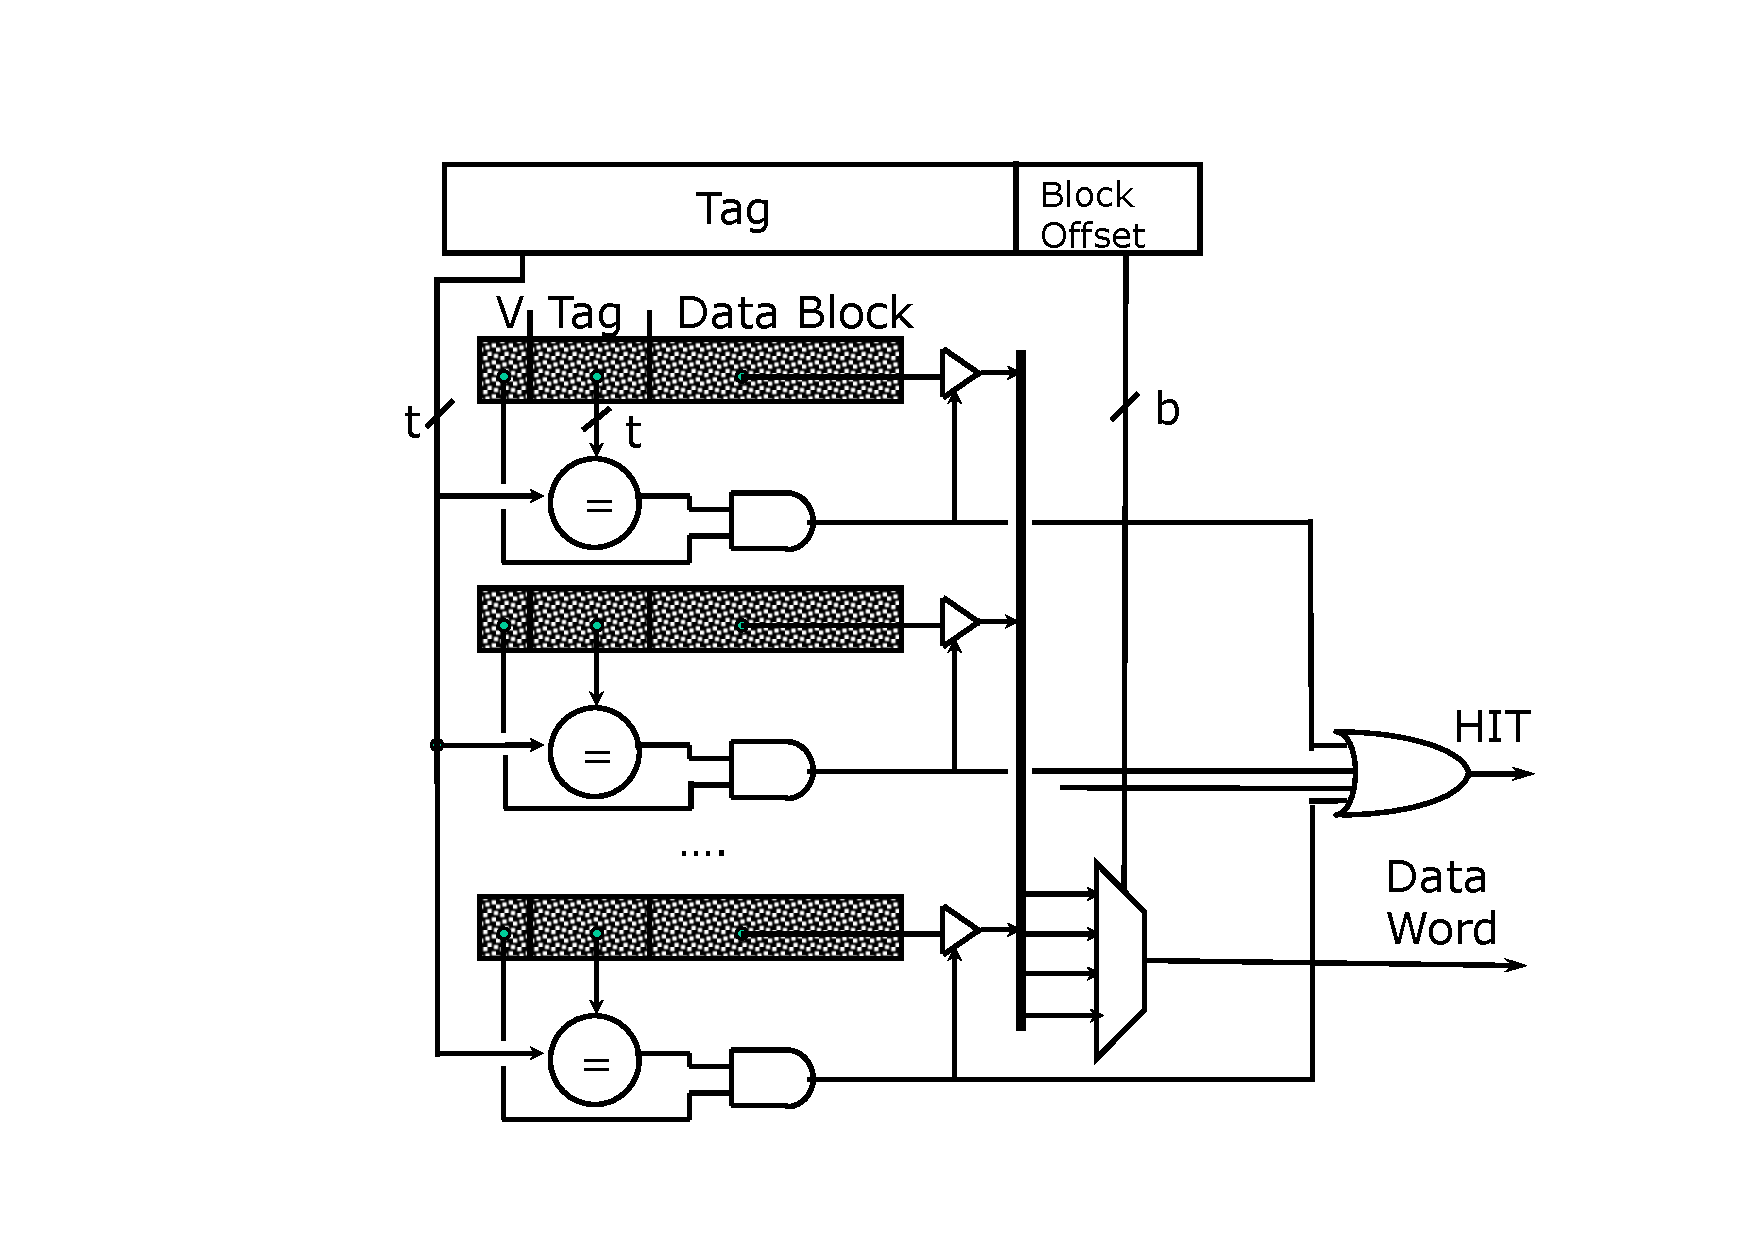
\includegraphics[width=.7\textwidth]{img/fully-associative-cache-2.pdf}
    \caption{The cache structure of the \emph{Fully Associative Cache} technique.}
    \label{fig: cache structure of the Fully Associative Cache}
\end{figure}

\noindent
As shown in Figure~\ref{fig: cache structure of the Fully Associative Cache}, the cache structure is more accessible because there are no \emph{Index} fields. We check only the \emph{Tag} field from the memory address. Finally, the \emph{Block Offset} chooses the \emph{Data Block} from the cache. We have a cache hit if the \emph{Tag} is equal to the \emph{Tag} of the cache and the value in and with the valid bit is true.

\newpage

\noindent
For \example{example}, we assume a block-frame address composed of 32 bits. Our cache structure is fully associative, and the number of cache blocks is 8. A possible exercise could be \textbf{determining where block 12 can be placed in the 8-block cache}.

\highspace
Unlike before, the position can be anywhere.

\begin{figure}[!htp]
    \centering
    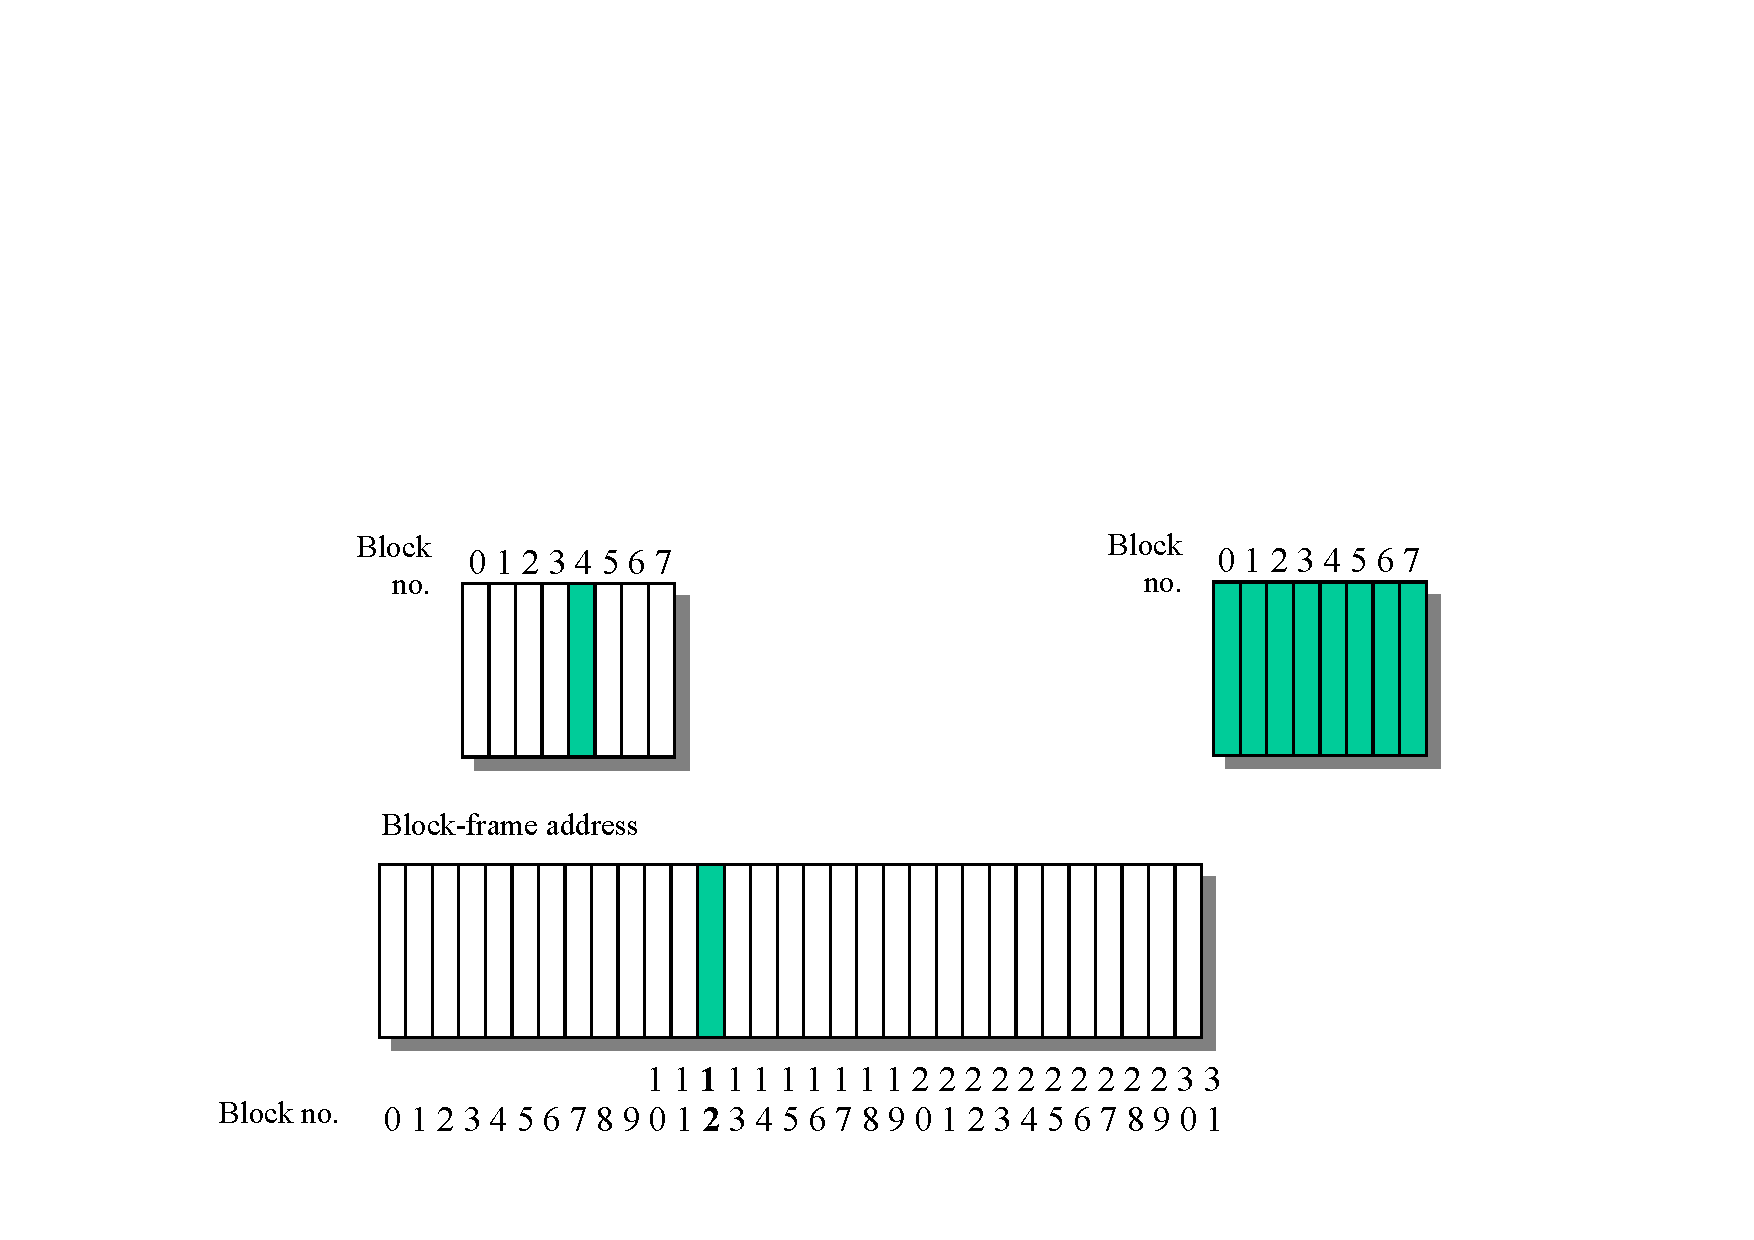
\includegraphics[width=.8\textwidth]{img/fully-associative-cache-3.pdf}
    \caption*{Direct Mapped on the left and Fully Associative on the right.}
\end{figure}

\newpage

\label{n-way Set Associative Cache}
\hypertarget{n-way Set Associative Cache}{\subsubsection*{\textcolor{Red2}{\emph{n}-way Set Associative Cache}}}

In a \definition{\emph{n}-way Set Associative Cache}, the \textbf{cache is composed of sets}. Each set is composed of \emph{n} blocks:
\begin{equation}
    \begin{array}{rcl}
        \texttt{Number of blocks} &=& \dfrac{\texttt{Cache Size}}{\texttt{Block Size}} \\ [1.5em]
        \texttt{Number of sets} &=& \dfrac{\texttt{Cache Size}}{\left(\texttt{Block Size} \times n\right)}
    \end{array}
\end{equation}
The memory block can be placed in any block of the set, so the \emph{search must be done on all the blocks}.

\highspace
\textbf{Each memory block corresponds to a single set of the cache}, and the \textbf{block can be placed in whatever block of the \emph{n} blocks of the set}:
\begin{equation}\label{eq: set cache}
    \left(\texttt{Set}\right)_{\texttt{cache}} = \left(\texttt{Block address}\right)_{\texttt{mem}} \texttt{mod} \left(\texttt{\# sets in cache}\right)
\end{equation}

\begin{figure}[!htp]
    \centering
    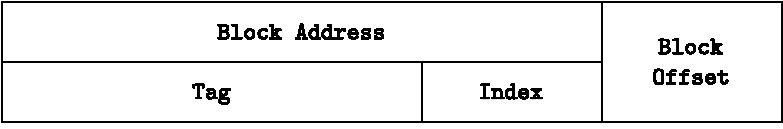
\includegraphics[width=.8\textwidth]{img/direct-mapped-cache-1.pdf}
    \caption{The memory address comprises the block address (Tag and index used to identify the set) and the block offset.}
\end{figure}

\begin{figure}[!htp]
    \centering
    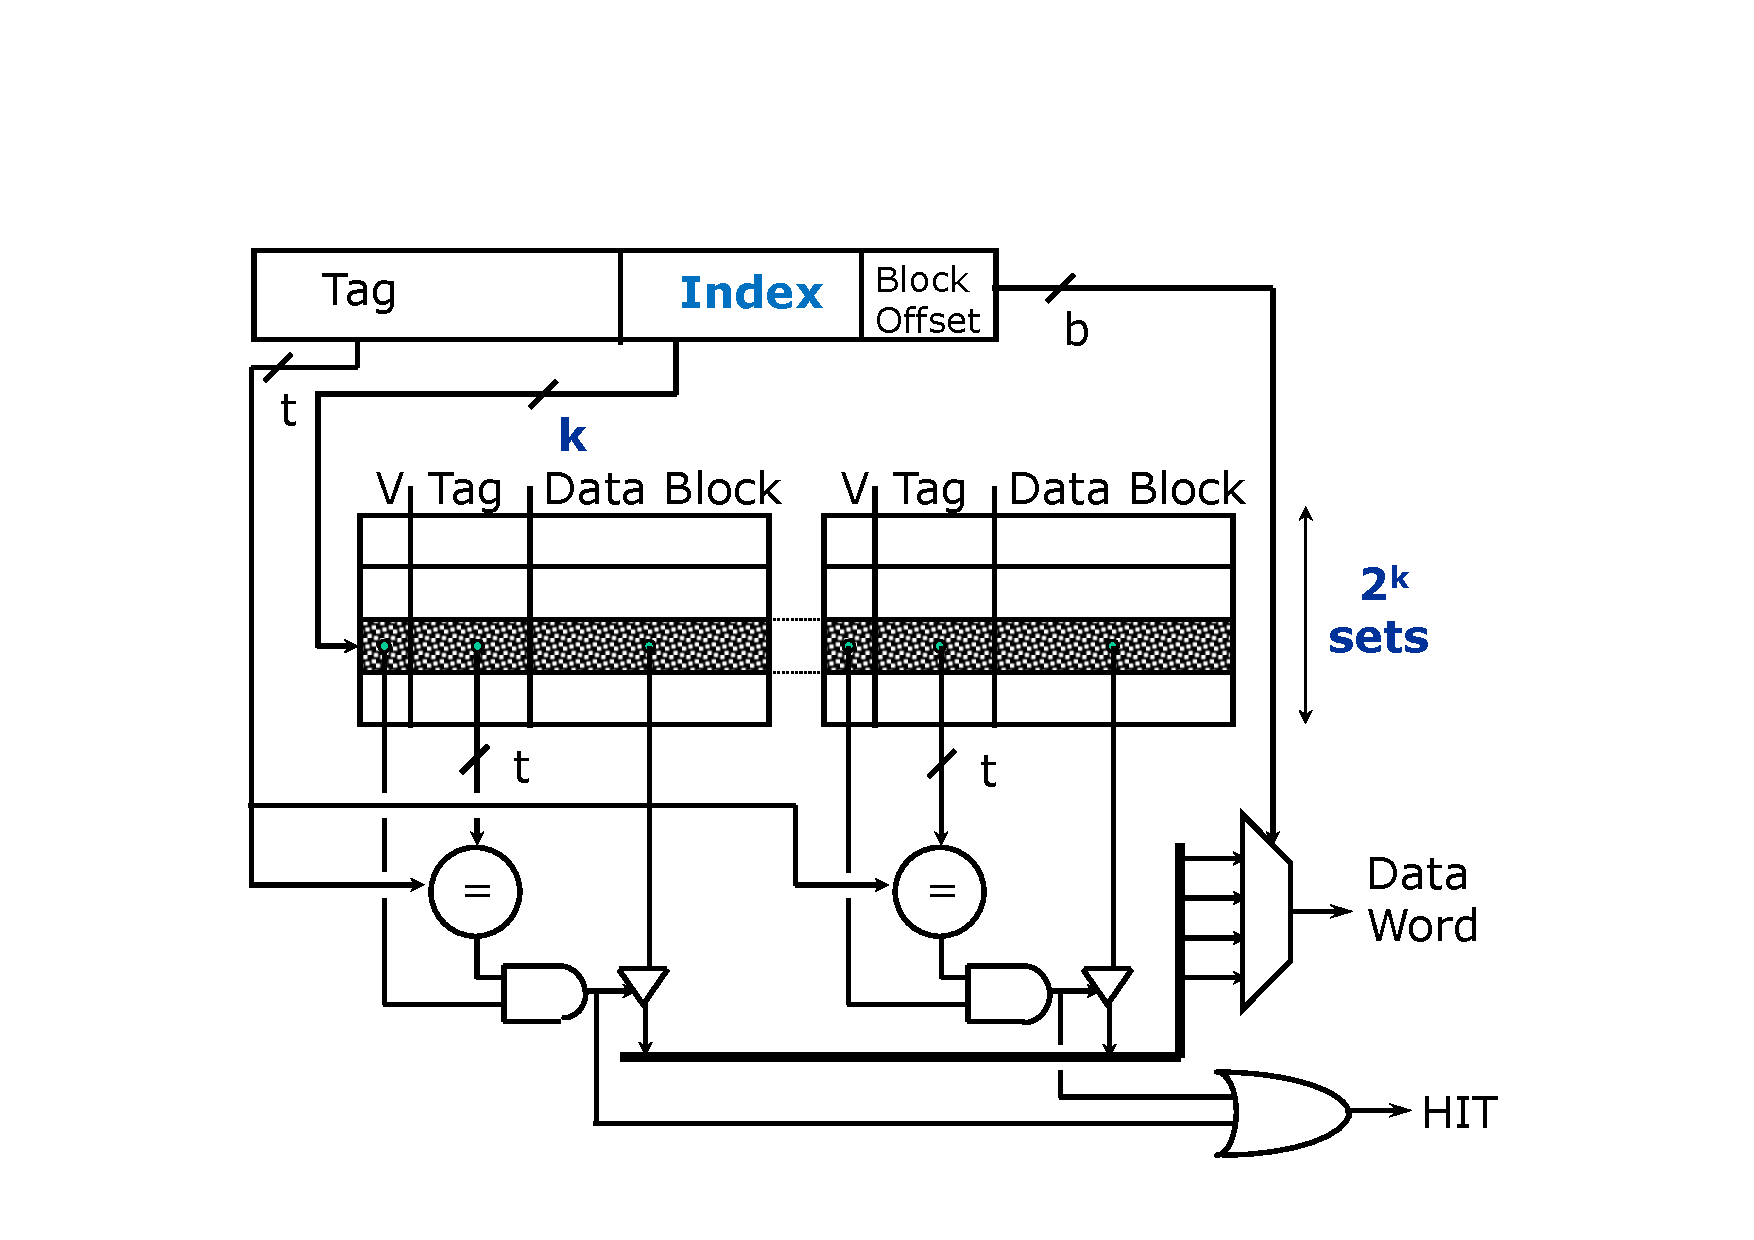
\includegraphics[width=.7\textwidth]{img/n-way-set-associative-cache-1.pdf}
    \caption{This structure is a \textbf{2-way Set Associative Cache}.}
\end{figure}

\newpage

\noindent
Taking the \example{examples} of previous pages, with the 2-way Set Associative, the answer is anywhere in set $0$. The reason for this is that using the formula~\ref{eq: set cache}:
\begin{equation*}
    \left(\texttt{Set}\right)_{\texttt{cache}} = 12 \mod 4 = 0
\end{equation*}

\begin{figure}[!htp]
    \centering
    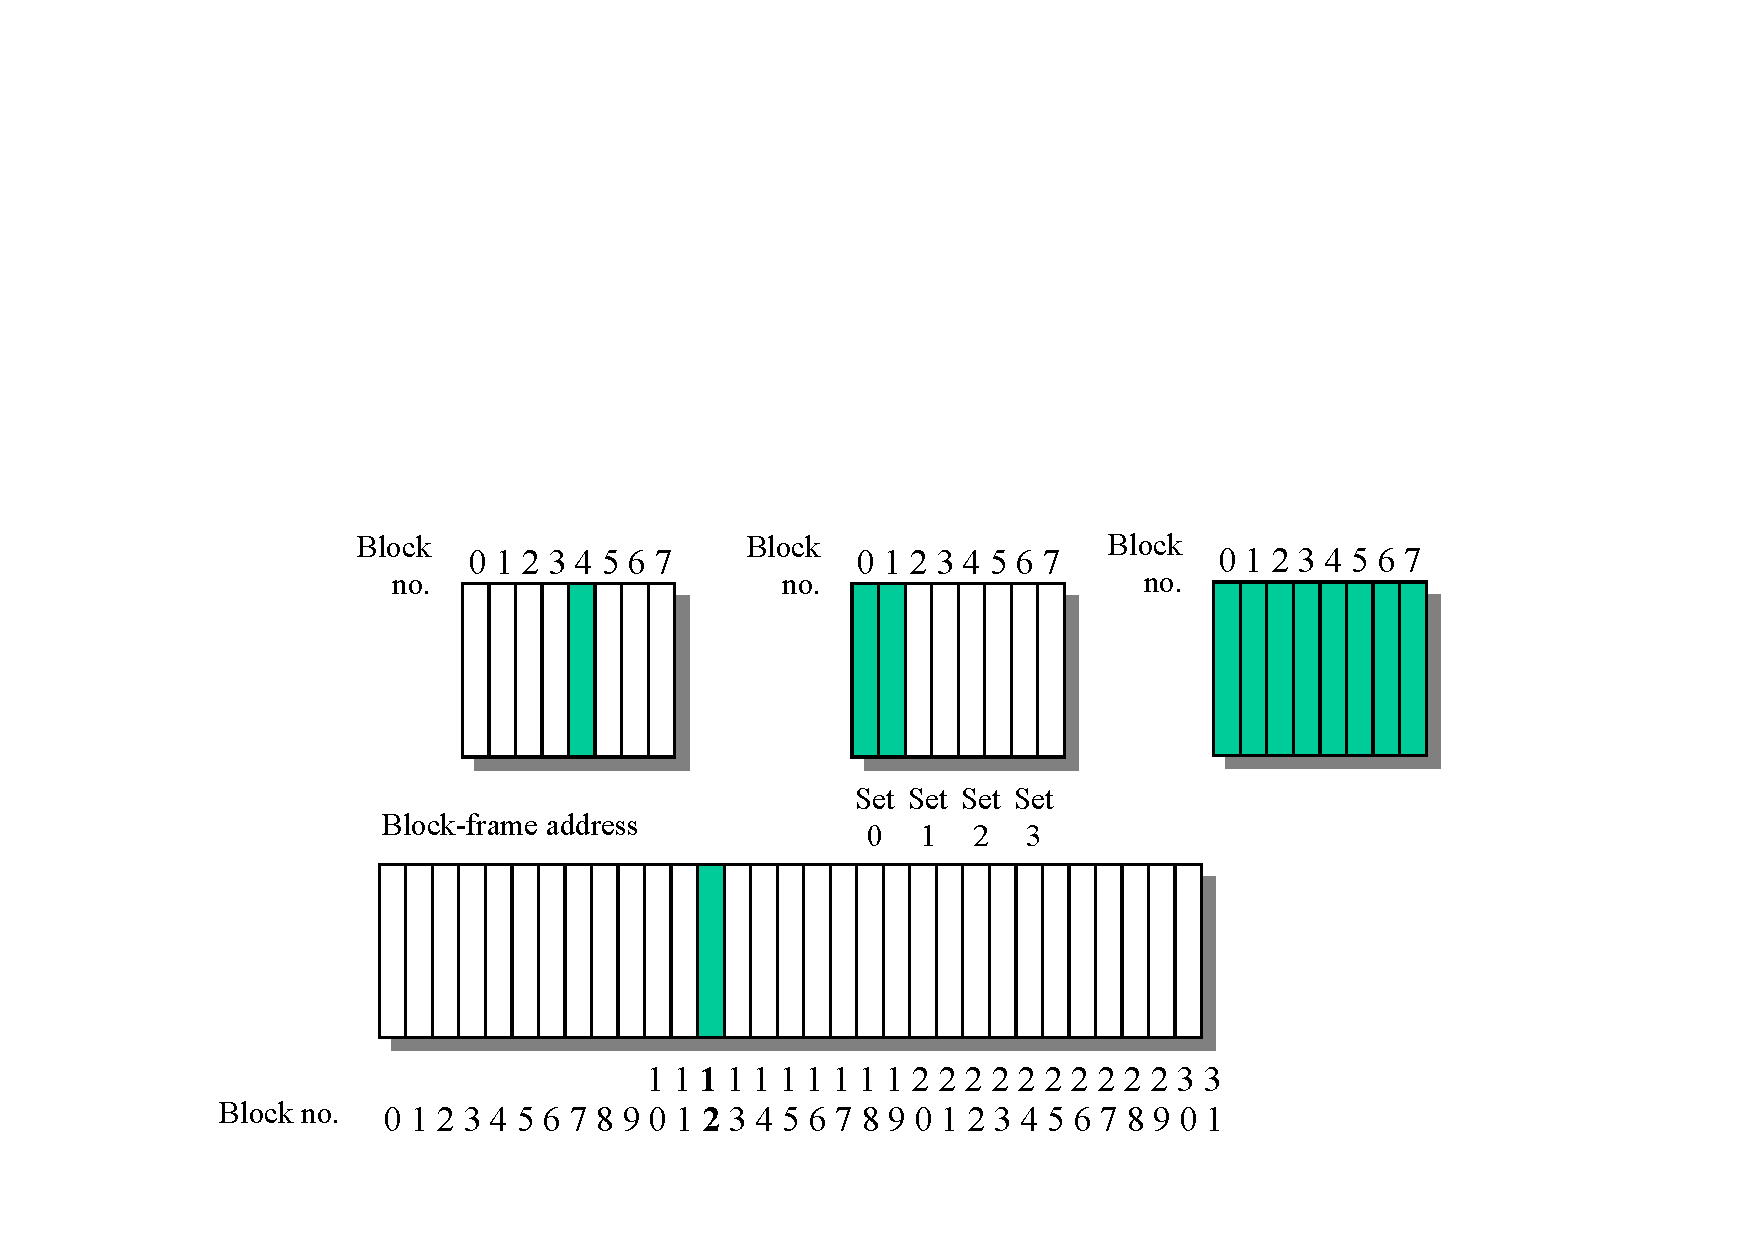
\includegraphics[width=\textwidth]{img/n-way-set-associative-cache-2.pdf}
    \caption*{Direct Mapped on the left, 2-way Set Associative on the center and Fully Associative on the right.}
\end{figure}

\newpage

\begin{center}
    \large
    \label{Block identification}
    \hypertarget{Block identification}{\textcolor{Red2}{\textbf{Block identification}}}
\end{center}

\noindent
The main question is: \emph{how is a block found if it is in the upper level?} The problem with identifying a block is that we must compare Tag bits. The comparison depends on the structure of the cache:
\begin{itemize}
    \item With \textbf{Direct Mapping} (page \pageref{Direct Mapped Cache}), we need to:
    \begin{itemize}
        \item Identify block positions by index (with the formula~\ref{eq: direct mapped cache});

        \item Compare block tags;
        
        \item Verify the valid bit.
    \end{itemize}

    \item With the \textbf{Set Associative Mapping} (page \pageref{n-way Set Associative Cache}), we need to:
    \begin{itemize}
        \item Identify the set by index (with the formula~\ref{eq: set cache});

        \item Compare tags of the set;

        \item Verify the Valid bit.
    \end{itemize}

    \item With the \textbf{Fully Associative Mapping} (page \pageref{Fully Associative Cache}), we must:
    \begin{itemize}
        \item Compare tags in \emph{every} block;
        
        \item Verify the Valid bit.
    \end{itemize}
\end{itemize}
Comparing the Tag bits, we do not need to check index or block offset bits.

\hfill

\longline

\hfill

\begin{center}
    \large
    \label{Block replacement}
    \hypertarget{Block replacement}{\textcolor{Red2}{\textbf{Block replacement}}}
\end{center}

\noindent
The main question is: \emph{which block should be replaced on a miss?} In case of a miss (definition on page~\pageref{definition: Cache Miss}), the replacement strategy depends on the structure of the cache:
\begin{itemize}
    \item In a \textbf{Fully Associative Cache} (page \pageref{Fully Associative Cache}), we need to decide which block to replace: any block is a potential candidate for the replacement.

    \item In a \textbf{Set Associative Cache} (page \pageref{n-way Set Associative Cache}), we must select among the blocks in the given set.
    
    \item In a \textbf{Direct Mapped Cache} (page \pageref{Direct Mapped Cache}), only one candidate must be replaced (\underline{no need} for any block replacement \underline{strategy}).
\end{itemize}
So in the \textbf{Fully Associative Cache} and \textbf{Set Associative Cache}, the \textbf{main strategies used to choose the block to be replaced} are:
\begin{itemize}
    \item \href{https://en.wikipedia.org/wiki/Cache_replacement_policies#Random_replacement_(RR)}{Random} (or \textbf{pseudo-random})
    
    \item \href{https://en.wikipedia.org/wiki/Cache_replacement_policies#Least_recently_used_(LRU)}{LRU (Least Recently Used)}

    \item \href{https://en.wikipedia.org/wiki/Cache_replacement_policies#First_in_first_out_(FIFO)}{FIFO (First In First Out, or oldest block replaced)}
\end{itemize}

\newpage

\begin{center}
    \large
    \label{Write strategy}
    \hypertarget{Write strategy}{\textcolor{Red2}{\textbf{Write strategy}}}
\end{center}

\noindent
The main question is: \emph{what happens on a write?} It depends on the written policy adopted in the cache. We remember that there are two possible options:
\begin{itemize}
    \item \definition{Write-Through}: \textbf{data is simultaneously updated} (written) \textbf{to cache and memory}. This process is more straightforward and more reliable. This is used when there are no frequent writes to the cache.
    
    \textcolor{Green3}{\faIcon{check} \textbf{The main advantages}}
    \begin{enumerate}
        \item It is \textbf{simpler to implement} but to be effective, it \emph{requires a write buffer} to not wait for the memory hierarchy (to avoid write stalls).

        \item The \textbf{read misses are cheaper} because they do not require any write to the memory hierarchy.

        \item \textbf{Memory is always up to date}. 
    \end{enumerate}


    \item \definition{Write-Back}: the \textbf{data is updated only in the cache and then added to the memory later}. The modified cache block is written to the memory only when it is replaced due to a cache miss. So, how can we understand if a block is clean or dirty? We need to add a \definition{Dirty Bit}. \textbf{Each Block in the cache requires a bit to indicate if the data present in the cache was modified} (\emph{Dirty}) \textbf{or not modified} (\emph{Clean}). If it is clean, writing it into the memory is unnecessary. It is designed to reduce write operation to a memory.

    \textcolor{Green3}{\faIcon{check} \textbf{The main advantages}}
    \begin{enumerate}
        \item The \textbf{processor can write the Block at the frequency the cache}, not the main memory, can accept.

        \item \textbf{Multiple writes to the same Block require only a single write to the main memory}.
    \end{enumerate}
\end{itemize}

\begin{flushleft}
    \textcolor{Red2}{\faIcon{question-circle} \textbf{What is a Write Buffer?}}
\end{flushleft}

\noindent
A \definition{Write Buffer} is a \textbf{FIFO buffer that does not wait for main memory access} (the typical number of entries is 4 to 8). So, the processor writes data to the cache and the write buffer; the memory controller writes the contents of the buffer to memory.

\begin{figure}[!htp]
    \centering
    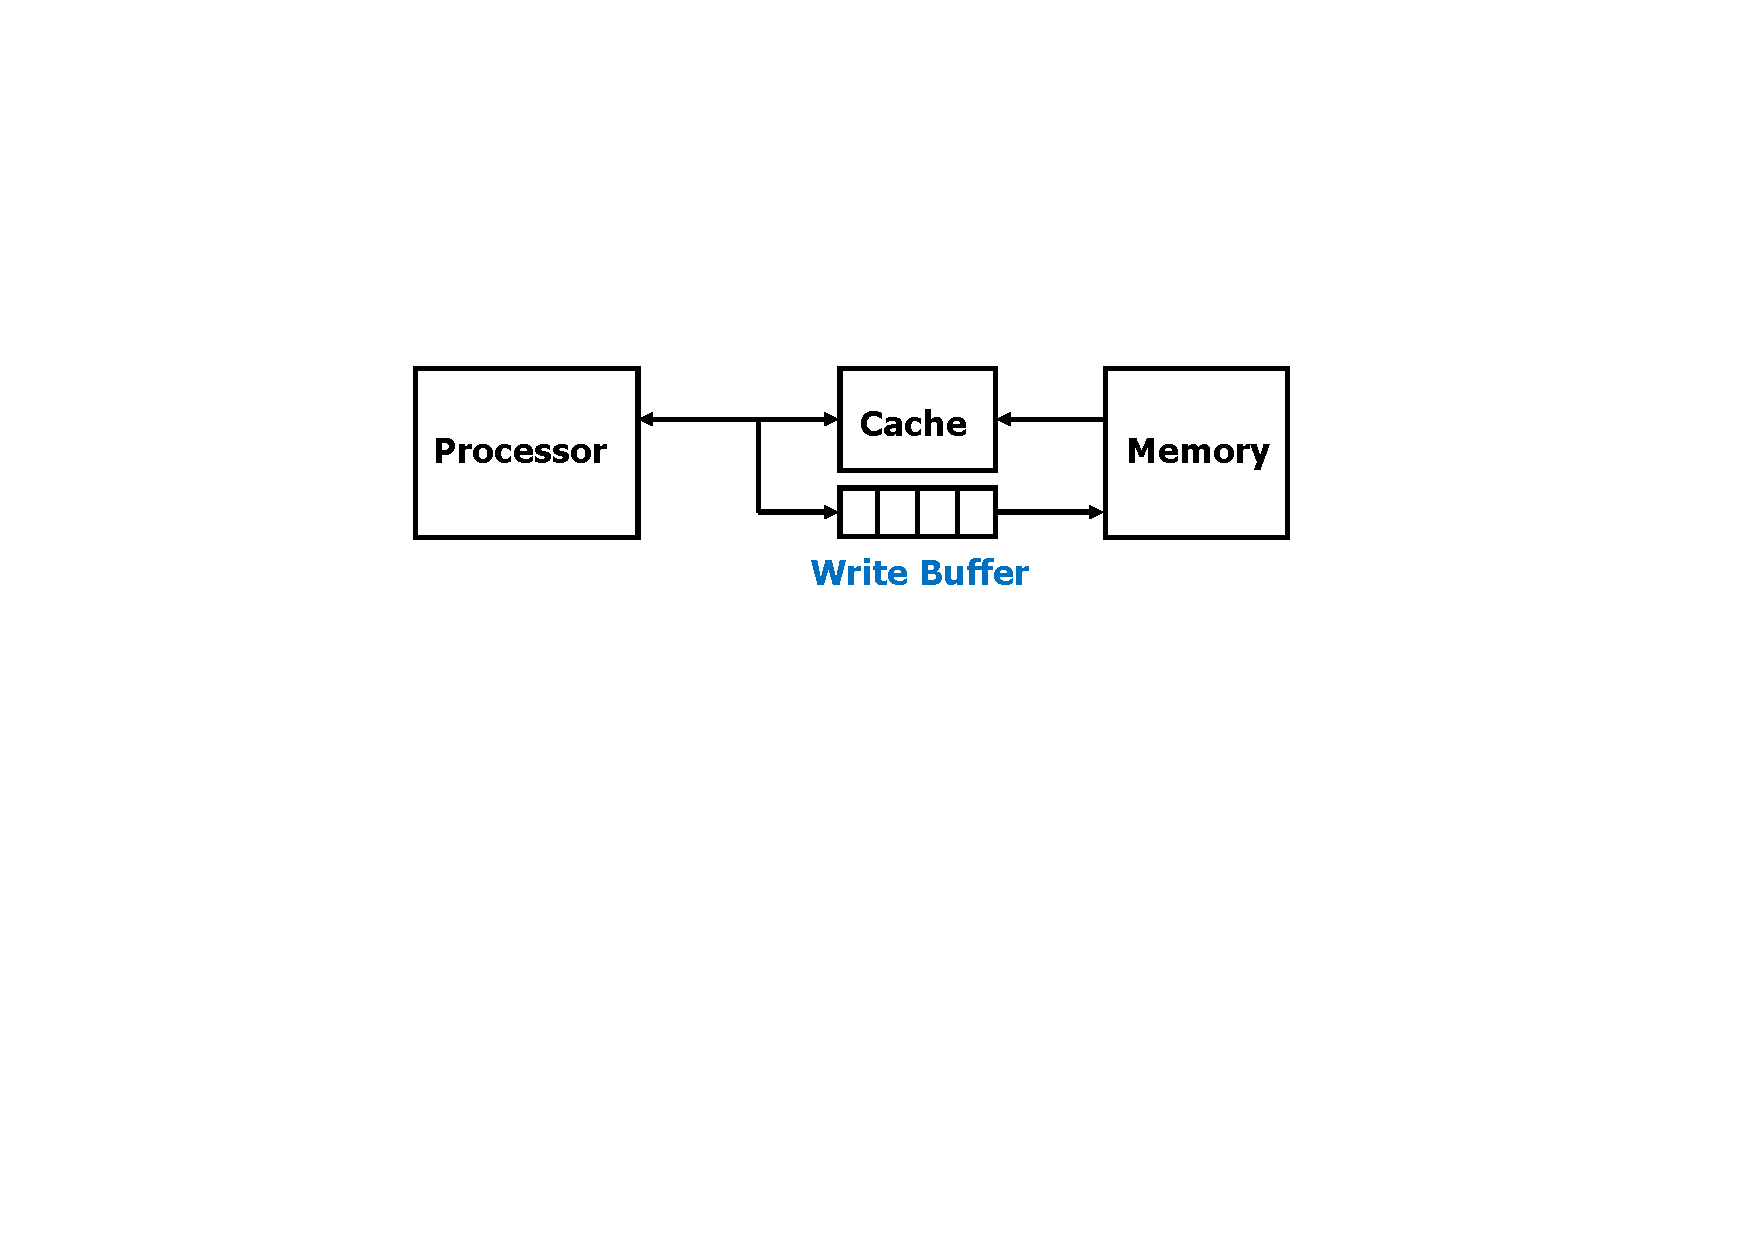
\includegraphics[width=.8\textwidth]{img/write-buffer-1.pdf}
    \caption{The cache structure with a Write Buffer.}
\end{figure}

\noindent
The \textbf{main problem with this idea is saturation}. However, as we have cited before, the write buffer is usually combined with the Write-Through policy.

\newpage

\begin{flushleft}
    \textcolor{Red2}{\faIcon{question-circle} \textbf{Ok, the cache can adopt one of the two write policies, but what happens on a Write Miss?}}
\end{flushleft}

\noindent
If write occurs to a location that is not present in the Cache (Write Miss), we use two options: \definition{Write Allocate} (or \emph{fetch on write}) and \definition{No Write Allocate} (\emph{Write-Around}). 

\highspace
In the first one, the \textbf{data is loaded from the memory into the cache and then updated}. Write Allocate works with both Write Back and Write-Through. However, it is \textbf{generally used with Write Back} because bringing data from the memory to the cache is unnecessary and then updating it in both the cache and main memory.

\highspace
In the \textbf{No Write Allocate} option, the \textbf{data is directly written/updated to the main memory without disturbing the cache}. It is better to use this when the data is not immediately used again. Generally, the \textbf{Write-Through cache uses the No Write Allocate} option (hoping the next writes to the Block will be done again in memory).

\newpage

\begin{flushleft}
    \textcolor{Green3}{\faIcon{clipboard-list} \textbf{Summary}}
\end{flushleft}

\begin{table}[!htp]
    \centering
    \begin{tabular}{@{} l p{20em} @{}}
        \toprule
        \textbf{Event} & \textbf{Summary} \\
        \midrule
        \textbf{Read Hit}   & Read data in cache. \\ [.5em]
        \textbf{Read Miss}  & Events that manifest themselves:
        \begin{enumerate}
            \item CPU stalls;
            \item Data request to memory;
            \item Copy in cache (write in cache);
            \item Repeat of cache read operation.
        \end{enumerate} \\
        \cmidrule{1-2}
        \textbf{Write Hit}  & It depends on the policy chosen:
        \begin{itemize}
            \item \emph{Write-Through}: write data both in cache and in memory.
            \item \emph{Write-Back}: write data to cache only, and copy memory only when replaced due to a cache miss.
        \end{itemize} \\ [.5em]
        \textbf{Write Miss} & There will certainly be CPU stalls. It also depends on the option we choose:
        \begin{itemize}
            \item \emph{Write Allocate}:
            \begin{enumerate}
                \item Data request to memory;
                \item Copy in cache (write in cache);
                \item Repeat of cache write operation.
            \end{enumerate}
            \item \emph{No Write Allocate}:
            \begin{enumerate}
                \item Simply send write data to main memory.
            \end{enumerate}
        \end{itemize} \\
        \bottomrule
    \end{tabular}
    \caption{Summary: Hit and Miss \& Read and Write.}
\end{table}
    \section{Software Configuration Management}

\subsection{Introduction}

\href{https://www.atlassian.com/microservices/microservices-architecture/configuration-management}{Configuration Management (CM)} is a systems engineering process for establishing consistency of a product's attributes throughout its life. In the technology world, configuration management is an IT management process that tracks individual configuration items of an IT system. IT systems are composed of IT assets that vary in granularity. An IT asset may represent a piece of software, or a server, or a cluster of servers. The following focuses on configuration management as it directly applies to IT software assets and software asset CI/CD.

\highspace
\definition{Software Configuration Management} is a \textbf{systems engineering process that tracks and monitors changes to a software systems configuration metadata}. In software development, configuration management is commonly used alongside version control and CI/CD infrastructure (explained later).

\highspace
The basic \textbf{approach to using a decentralized CM} is to have a repository (project) on the server side. 
\begin{itemize}
    \item When we want to work on the project, we clone the repository on the local PC. This workflow is used because we can work offline and on the local project without making critical changes to the repository server side.
    
    \item The local changes can be saved using the commit command and when we are ready to publish our changes, we use the push command to update the repository on the server side.
    
    \item After a push, anyone who has a local copy should make a pull command to update the local project.
\end{itemize}
This workflow can be done using git commands, and a good cheat sheet can be found \href{https://education.github.com/git-cheat-sheet-education.pdf}{here}.
    \subsubsection{Interrupts and Interrupt Handler}

The \textbf{interrupts change the normal flow of control}. As you can see in Figure \ref{fig: Program and Interrupt Handler}, on the left we see the instructions of the program; on the right we see the interrupt handler.

\begin{figure}[!htp]
    \centering
    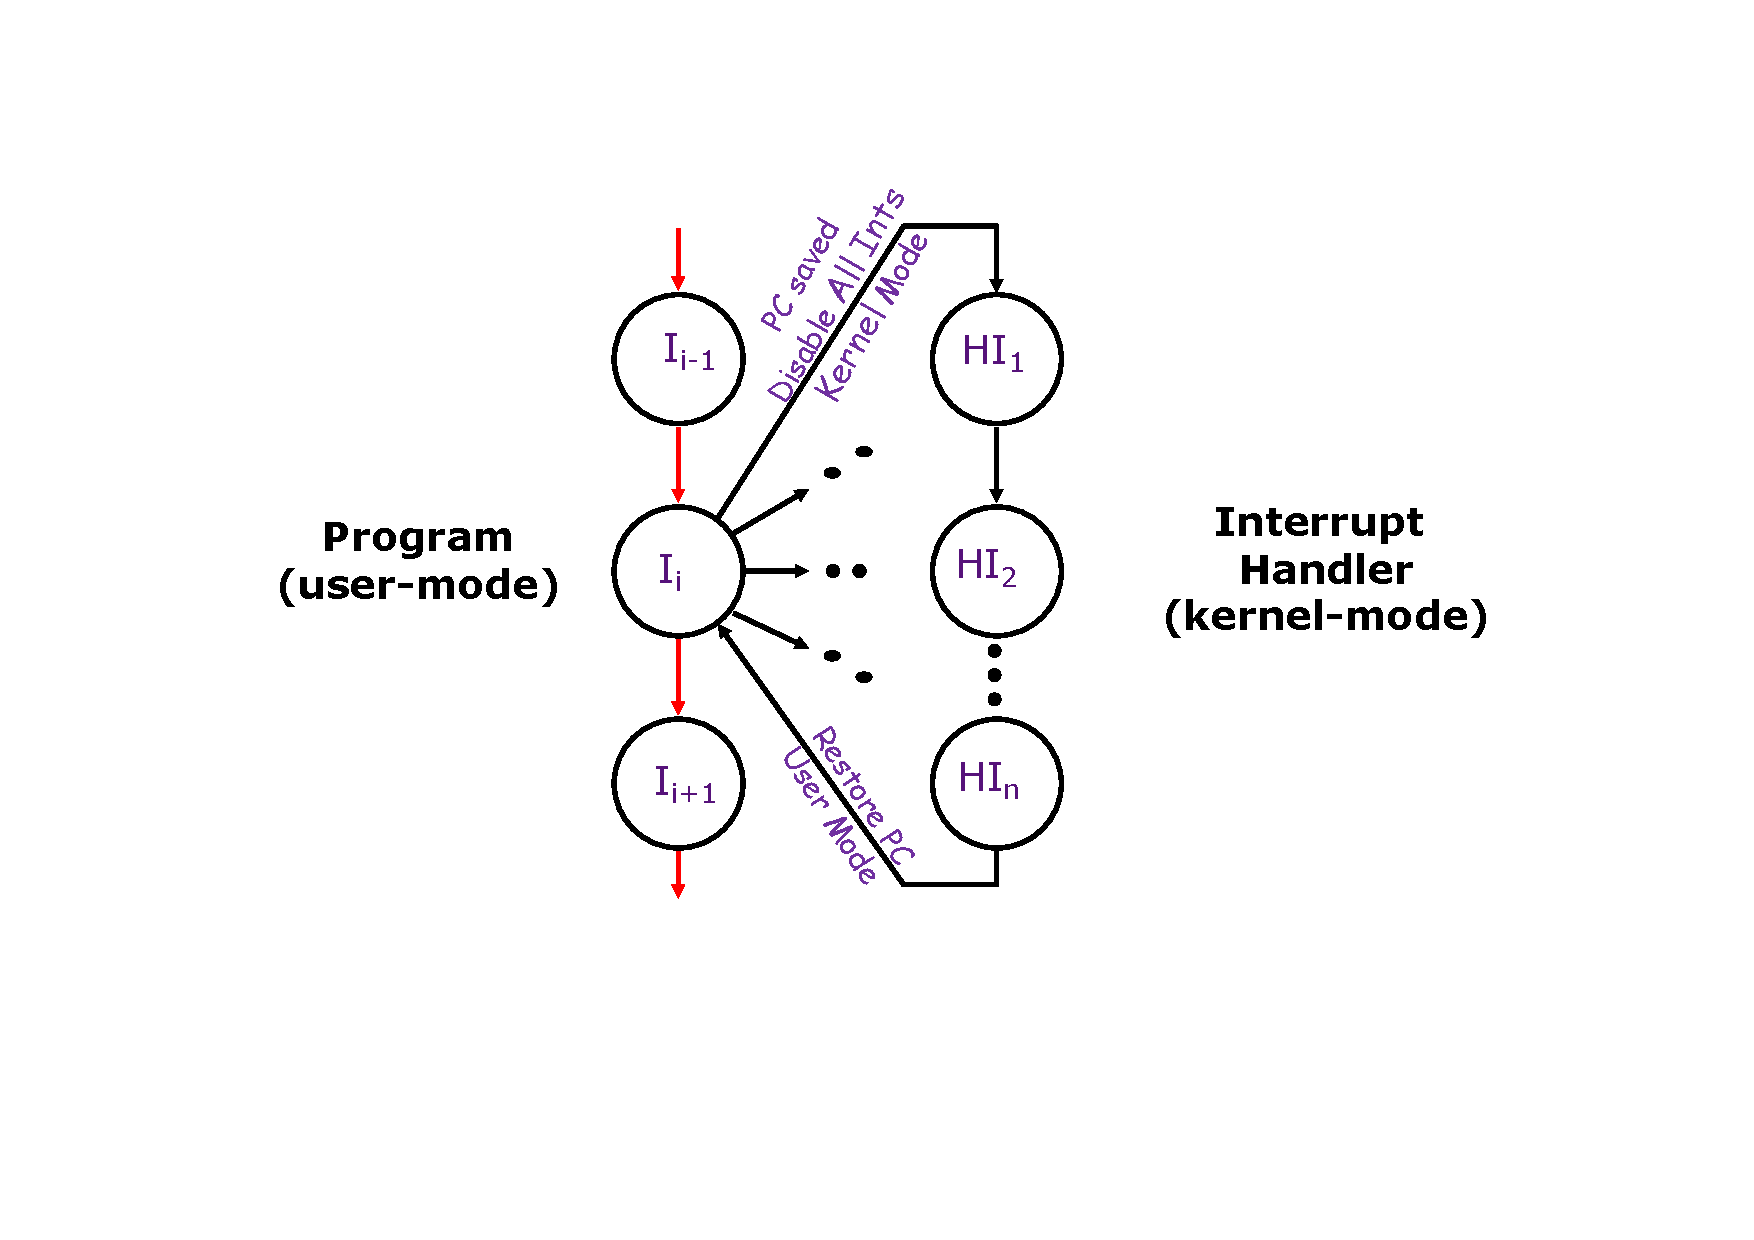
\includegraphics[width=.8\textwidth]{img/interrupts-1.pdf}
    \caption{Program and Interrupt Handler.}
    \label{fig: Program and Interrupt Handler}
\end{figure}

\noindent
An \indexdefinition{Interrupt Handler}, also known as an \textbf{interrupt service routine} or \textbf{ISR}, is a special \textbf{block of code associated with a specific interrupt condition}. Interrupts can be of two types:
\begin{itemize}
    \item \indexdefinition{Synchronous Interrupts} (exception) are caused by a particular instruction stage. In general, the \textbf{instruction} $I_{i}$ (see the Figure \ref{fig: Program and Interrupt Handler}) \textbf{cannot be completed} and needs to be \textbf{restarted after the exception has been handled}.
    
    If we think about the pipeline, this condition requires undoing the effect of one or more partially executed instructions.


    \item \indexdefinition{Asynchronous Interrupts} are caused by an I/O device requesting attention by asserting one of the prioritized interrupt request lines.
    
    When the processor decides to process the interrupt:
    \begin{enumerate}
        \item It stops the current program at instruction $I_{i}$, completing all the instructions up to $I_{i-1}$ (called \textbf{precise interrupt}, see below to understand what it is).
        
        \item It saves the Program Counter (PC) of the instruction $I_{i}$ in a special register called \indexdefinition{Exception Program Counter (EPC)}: $\texttt{PC} \rightarrow \texttt{EPC}$.
        
        \item It disables interrupts and transfer control to a designated interrupt handler running in the \textbf{kernel mode}. So it loads the \indexdefinition{Interrupt Vector Address (IVA)} into the Program Counter (PC): $\texttt{IVA} \rightarrow \texttt{PC}$.
        
        \newpage

        \item When the Interrupt Handler has finished, it must \textbf{restore the stable situation}. It uses a \textbf{special indirect jump instruction} called \indexdefinition{Return-From-Exception (RFE)}, which restores the PC and:
        \begin{itemize}
            \item Re-enables the interrupts (again, because they were disabled in the previous step);
            
            \item Returns the processor to user mode;
            
            \item Restores the hardware and control state.
        \end{itemize}
    \end{enumerate}
\end{itemize}

\begin{flushleft}
    \textcolor{Green4}{\faIcon{question-circle} \textbf{Ok, but what exactly is a Precise Interrupts in Asynchronous Interrupts?}}
\end{flushleft} \index{Precise Interrupts}\index{Precise Exceptions}
An \textbf{interrupt} or \textbf{exception} is \textbf{precise} if there is a single instruction (or interrupt point) for which all \textbf{previous instructions} have \textbf{committed their state} and \textbf{no subsequent instructions} (including the interrupting instruction $I_{i}$) have \textbf{changed any state}.

\highspace
In other words, we can restart execution at the interrupt point and \dquotes{get the right answer}.

\begin{figure}[!htp]
    \centering
    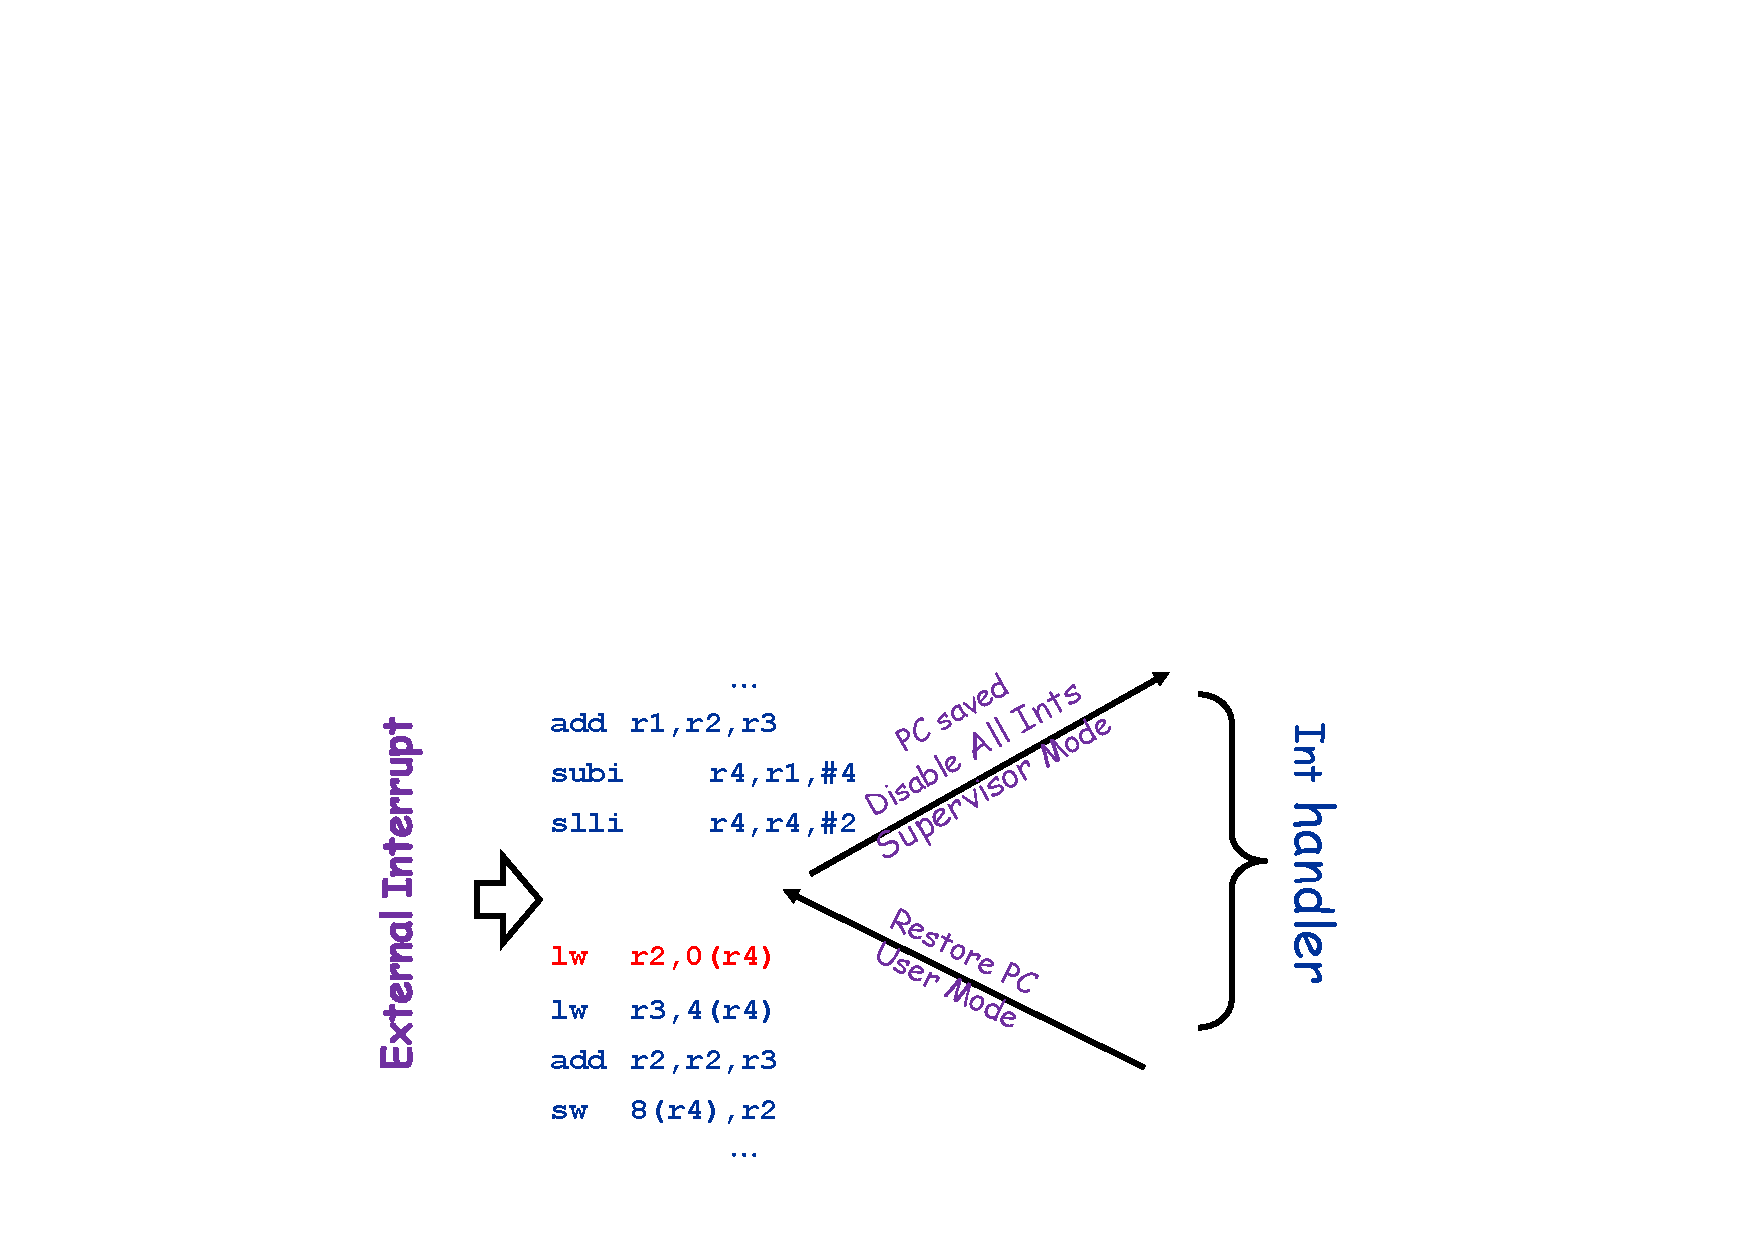
\includegraphics[width=.8\textwidth]{img/precise-interrupts-1.pdf}
    \caption{\example{Example} of precise interrupt/exception (interrupt point is at red \texttt{lw} instruction).}
\end{figure}

    %%%%%%%%%%%%%%%%%%%%%%%%%
    % Clear fancy pagestyle %
    %%%%%%%%%%%%%%%%%%%%%%%%%
    \pagestyle{fancy}
    \fancyhead{} % clear all header fields
    \fancyhead[R]{\nouppercase{\leftmark}}

    %%%%%%%%%%%%%%%%%%%%%%%%%%
    % Bibliography and index %
    %%%%%%%%%%%%%%%%%%%%%%%%%%
    \bibliography{bibtex}{}
\bibliographystyle{plain}

\newpage

\printindex
\end{document}